% Template for PLoS
%DIF LATEXDIFF DIFFERENCE FILE
%DIF DEL Journal-manuscriptV0.tex   Thu Feb  1 10:49:35 2024
%DIF ADD Journal-manuscript.tex     Thu Feb  1 11:11:20 2024
% Version 3.5 March 2018
%
% % % % % % % % % % % % % % % % % % % % % %
%
% -- IMPORTANT NOTE
%
% This template contains comments intended
% to minimize problems and delays during our production
% process. Please follow the template instructions
% whenever possible.
%
% % % % % % % % % % % % % % % % % % % % % % %
%
% Once your paper is accepted for publication,
% PLEASE REMOVE ALL TRACKED CHANGES in this file
% and leave only the final text of your manuscript.
% PLOS recommends the use of latexdiff to track changes during review, as this will help to maintain a clean tex file.
% Visit https://www.ctan.org/pkg/latexdiff?lang=en for info or contact us at latex@plos.org.
%
%
% There are no restrictions on package use within the LaTeX files except that
% no packages listed in the template may be deleted.
%
% Please do not include colors or graphics in the text.
%
% The manuscript LaTeX source should be contained within a single file (do not use \input, \externaldocument, or similar commands).
%
% % % % % % % % % % % % % % % % % % % % % % %
%
% -- FIGURES AND TABLES
%
% Please include tables/figure captions directly after the paragraph where they are first cited in the text.
%
% DO NOT INCLUDE GRAPHICS IN YOUR MANUSCRIPT
% - Figures should be uploaded separately from your manuscript file.
% - Figures generated using LaTeX should be extracted and removed from the PDF before submission.
% - Figures containing multiple panels/subfigures must be combined into one image file before submission.
% For figure citations, please use "Fig" instead of "Figure".
% See http://journals.plos.org/plosone/s/figures for PLOS figure guidelines.
%
% Tables should be cell-based and may not contain:
% - spacing/line breaks within cells to alter layout or alignment
% - do not nest tabular environments (no tabular environments within tabular environments)
% - no graphics or colored text (cell background color/shading OK)
% See http://journals.plos.org/plosone/s/tables for table guidelines.
%
% For tables that exceed the width of the text column, use the adjustwidth environment as illustrated in the example table in text below.
%
% % % % % % % % % % % % % % % % % % % % % % % %
%
% -- EQUATIONS, MATH SYMBOLS, SUBSCRIPTS, AND SUPERSCRIPTS
%
% IMPORTANT
% Below are a few tips to help format your equations and other special characters according to our specifications. For more tips to help reduce the possibility of formatting errors during conversion, please see our LaTeX guidelines at http://journals.plos.org/plosone/s/latex
%
% For inline equations, please be sure to include all portions of an equation in the math environment.
%
% Do not include text that is not math in the math environment.
%
% Please add line breaks to long display equations when possible in order to fit size of the column.
%
% For inline equations, please do not include punctuation (commas, etc) within the math environment unless this is part of the equation.
%
% When adding superscript or subscripts outside of brackets/braces, please group using {}.
%
% Do not use \cal for caligraphic font.  Instead, use \mathcal{}
%
% % % % % % % % % % % % % % % % % % % % % % % %
%
% Please contact latex@plos.org with any questions.
%
% % % % % % % % % % % % % % % % % % % % % % % %

\documentclass[10pt,letterpaper]{article}
\usepackage[top=0.85in,left=2.75in,footskip=0.75in]{geometry}

% amsmath and amssymb packages, useful for mathematical formulas and symbols
\usepackage{amsmath,amssymb}

% Use adjustwidth environment to exceed column width (see example table in text)
\usepackage{changepage}


% textcomp package and marvosym package for additional characters
\usepackage{textcomp,marvosym}

% cite package, to clean up citations in the main text. Do not remove.
% \usepackage{cite}

% Use nameref to cite supporting information files (see Supporting Information section for more info)
\usepackage{nameref,hyperref}

% line numbers
\usepackage[right]{lineno}

% ligatures disabled
\usepackage{microtype}
\DisableLigatures[f]{encoding = *, family = * }

% color can be used to apply background shading to table cells only
\usepackage[table]{xcolor}

% array package and thick rules for tables
\usepackage{array}

% create "+" rule type for thick vertical lines
\newcolumntype{+}{!{\vrule width 2pt}}

% create \thickcline for thick horizontal lines of variable length
\newlength\savedwidth
\newcommand\thickcline[1]{%
  \noalign{\global\savedwidth\arrayrulewidth\global\arrayrulewidth 2pt}%
  \cline{#1}%
  \noalign{\vskip\arrayrulewidth}%
  \noalign{\global\arrayrulewidth\savedwidth}%
}

% \thickhline command for thick horizontal lines that span the table
\newcommand\thickhline{\noalign{\global\savedwidth\arrayrulewidth\global\arrayrulewidth 2pt}%
\hline
\noalign{\global\arrayrulewidth\savedwidth}}


% Remove comment for double spacing
%\usepackage{setspace}
%\doublespacing

% Text layout
\raggedright
\setlength{\parindent}{0.5cm}
\textwidth 5.25in
\textheight 8.75in

% Bold the 'Figure #' in the caption and separate it from the title/caption with a period
% Captions will be left justified
\usepackage[aboveskip=1pt,labelfont=bf,labelsep=period,justification=raggedright,singlelinecheck=off]{caption}
\renewcommand{\figurename}{Fig}

% Use the PLoS provided BiBTeX style
% \bibliographystyle{plos2015}

% Remove brackets from numbering in List of References
\makeatletter
\renewcommand{\@biblabel}[1]{\quad#1.}
\makeatother



% Header and Footer with logo
\usepackage{lastpage,fancyhdr,graphicx}
\usepackage{epstopdf}
%\pagestyle{myheadings}
\pagestyle{fancy}
\fancyhf{}
%\setlength{\headheight}{27.023pt}
%\lhead{
\includegraphics[width=2.0in]{PLOS-submission.eps}}
\rfoot{\thepage/\pageref{LastPage}}
\renewcommand{\headrulewidth}{0pt}
\renewcommand{\footrule}{\hrule height 2pt \vspace{2mm}}
\fancyheadoffset[L]{2.25in}
\fancyfootoffset[L]{2.25in}
\lfoot{\today}

%% Include all macros below

\newcommand{\lorem}{{\bf LOREM}}
\newcommand{\ipsum}{{\bf IPSUM}}


% tightlist command for lists without linebreak
\providecommand{\tightlist}{%
  \setlength{\itemsep}{0pt}\setlength{\parskip}{0pt}}


% Pandoc citation processing
\newlength{\cslhangindent}
\setlength{\cslhangindent}{1.5em}
\newlength{\csllabelwidth}
\setlength{\csllabelwidth}{3em}
\newlength{\cslentryspacingunit} % times entry-spacing
\setlength{\cslentryspacingunit}{\parskip}
% for Pandoc 2.8 to 2.10.1
\newenvironment{cslreferences}%
  {}%
  {\par}
% For Pandoc 2.11+
\newenvironment{CSLReferences}[2] % #1 hanging-ident, #2 entry spacing
 {% don't indent paragraphs
  \setlength{\parindent}{0pt}
  % turn on hanging indent if param 1 is 1
  \ifodd #1
  \let\oldpar\par
  \def\par{\hangindent=\cslhangindent\oldpar}
  \fi
  % set entry spacing
  \setlength{\parskip}{#2\cslentryspacingunit}
 }%
 {}
\usepackage{calc}
\newcommand{\CSLBlock}[1]{#1\hfill\break}
\newcommand{\CSLLeftMargin}[1]{\parbox[t]{\csllabelwidth}{#1}}
\newcommand{\CSLRightInline}[1]{\parbox[t]{\linewidth - \csllabelwidth}{#1}\break}
\newcommand{\CSLIndent}[1]{\hspace{\cslhangindent}#1}

\usepackage{multirow}
\usepackage{multicol}
\usepackage{colortbl}
\usepackage{hhline}
\newlength\Oldarrayrulewidth
\newlength\Oldtabcolsep
\usepackage{longtable}
\usepackage{array}
\usepackage{hyperref}
\usepackage{float}
\usepackage{wrapfig}


\usepackage{forarray}
\usepackage{xstring}
\newcommand{\getIndex}[2]{
  \ForEach{,}{\IfEq{#1}{\thislevelitem}{\number\thislevelcount\ExitForEach}{}}{#2}
}

\setcounter{secnumdepth}{0}

\newcommand{\getAff}[1]{
  \getIndex{#1}{McMaster,Madrid}
}
%DIF PREAMBLE EXTENSION ADDED BY LATEXDIFF
%DIF UNDERLINE PREAMBLE %DIF PREAMBLE
\RequirePackage[normalem]{ulem} %DIF PREAMBLE
\RequirePackage{color}\definecolor{RED}{rgb}{1,0,0}\definecolor{BLUE}{rgb}{0,0,1} %DIF PREAMBLE
\providecommand{\DIFaddtex}[1]{{\protect\color{blue}\uwave{#1}}} %DIF PREAMBLE
\providecommand{\DIFdeltex}[1]{{\protect\color{red}\sout{#1}}}                      %DIF PREAMBLE
%DIF SAFE PREAMBLE %DIF PREAMBLE
\providecommand{\DIFaddbegin}{} %DIF PREAMBLE
\providecommand{\DIFaddend}{} %DIF PREAMBLE
\providecommand{\DIFdelbegin}{} %DIF PREAMBLE
\providecommand{\DIFdelend}{} %DIF PREAMBLE
\providecommand{\DIFmodbegin}{} %DIF PREAMBLE
\providecommand{\DIFmodend}{} %DIF PREAMBLE
%DIF FLOATSAFE PREAMBLE %DIF PREAMBLE
\providecommand{\DIFaddFL}[1]{\DIFadd{#1}} %DIF PREAMBLE
\providecommand{\DIFdelFL}[1]{\DIFdel{#1}} %DIF PREAMBLE
\providecommand{\DIFaddbeginFL}{} %DIF PREAMBLE
\providecommand{\DIFaddendFL}{} %DIF PREAMBLE
\providecommand{\DIFdelbeginFL}{} %DIF PREAMBLE
\providecommand{\DIFdelendFL}{} %DIF PREAMBLE
%DIF HYPERREF PREAMBLE %DIF PREAMBLE
\providecommand{\DIFadd}[1]{\texorpdfstring{\DIFaddtex{#1}}{#1}} %DIF PREAMBLE
\providecommand{\DIFdel}[1]{\texorpdfstring{\DIFdeltex{#1}}{}} %DIF PREAMBLE
\newcommand{\DIFscaledelfig}{0.5}
%DIF HIGHLIGHTGRAPHICS PREAMBLE %DIF PREAMBLE
\RequirePackage{settobox} %DIF PREAMBLE
\RequirePackage{letltxmacro} %DIF PREAMBLE
\newsavebox{\DIFdelgraphicsbox} %DIF PREAMBLE
\newlength{\DIFdelgraphicswidth} %DIF PREAMBLE
\newlength{\DIFdelgraphicsheight} %DIF PREAMBLE
% store original definition of \includegraphics %DIF PREAMBLE
\LetLtxMacro{\DIFOincludegraphics}{\includegraphics} %DIF PREAMBLE
\newcommand{\DIFaddincludegraphics}[2][]{{\color{blue}\fbox{\DIFOincludegraphics[#1]{#2}}}} %DIF PREAMBLE
\newcommand{\DIFdelincludegraphics}[2][]{% %DIF PREAMBLE
\sbox{\DIFdelgraphicsbox}{\DIFOincludegraphics[#1]{#2}}% %DIF PREAMBLE
\settoboxwidth{\DIFdelgraphicswidth}{\DIFdelgraphicsbox} %DIF PREAMBLE
\settoboxtotalheight{\DIFdelgraphicsheight}{\DIFdelgraphicsbox} %DIF PREAMBLE
\scalebox{\DIFscaledelfig}{% %DIF PREAMBLE
\parbox[b]{\DIFdelgraphicswidth}{\usebox{\DIFdelgraphicsbox}\\[-\baselineskip] \rule{\DIFdelgraphicswidth}{0em}}\llap{\resizebox{\DIFdelgraphicswidth}{\DIFdelgraphicsheight}{% %DIF PREAMBLE
\setlength{\unitlength}{\DIFdelgraphicswidth}% %DIF PREAMBLE
\begin{picture}(1,1)% %DIF PREAMBLE
\thicklines\linethickness{2pt} %DIF PREAMBLE
{\color[rgb]{1,0,0}\put(0,0){\framebox(1,1){}}}% %DIF PREAMBLE
{\color[rgb]{1,0,0}\put(0,0){\line( 1,1){1}}}% %DIF PREAMBLE
{\color[rgb]{1,0,0}\put(0,1){\line(1,-1){1}}}% %DIF PREAMBLE
\end{picture}% %DIF PREAMBLE
}\hspace*{3pt}}} %DIF PREAMBLE
} %DIF PREAMBLE
\LetLtxMacro{\DIFOaddbegin}{\DIFaddbegin} %DIF PREAMBLE
\LetLtxMacro{\DIFOaddend}{\DIFaddend} %DIF PREAMBLE
\LetLtxMacro{\DIFOdelbegin}{\DIFdelbegin} %DIF PREAMBLE
\LetLtxMacro{\DIFOdelend}{\DIFdelend} %DIF PREAMBLE
\DeclareRobustCommand{\DIFaddbegin}{\DIFOaddbegin \let\includegraphics\DIFaddincludegraphics} %DIF PREAMBLE
\DeclareRobustCommand{\DIFaddend}{\DIFOaddend \let\includegraphics\DIFOincludegraphics} %DIF PREAMBLE
\DeclareRobustCommand{\DIFdelbegin}{\DIFOdelbegin \let\includegraphics\DIFdelincludegraphics} %DIF PREAMBLE
\DeclareRobustCommand{\DIFdelend}{\DIFOaddend \let\includegraphics\DIFOincludegraphics} %DIF PREAMBLE
\LetLtxMacro{\DIFOaddbeginFL}{\DIFaddbeginFL} %DIF PREAMBLE
\LetLtxMacro{\DIFOaddendFL}{\DIFaddendFL} %DIF PREAMBLE
\LetLtxMacro{\DIFOdelbeginFL}{\DIFdelbeginFL} %DIF PREAMBLE
\LetLtxMacro{\DIFOdelendFL}{\DIFdelendFL} %DIF PREAMBLE
\DeclareRobustCommand{\DIFaddbeginFL}{\DIFOaddbeginFL \let\includegraphics\DIFaddincludegraphics} %DIF PREAMBLE
\DeclareRobustCommand{\DIFaddendFL}{\DIFOaddendFL \let\includegraphics\DIFOincludegraphics} %DIF PREAMBLE
\DeclareRobustCommand{\DIFdelbeginFL}{\DIFOdelbeginFL \let\includegraphics\DIFdelincludegraphics} %DIF PREAMBLE
\DeclareRobustCommand{\DIFdelendFL}{\DIFOaddendFL \let\includegraphics\DIFOincludegraphics} %DIF PREAMBLE
%DIF COLORLISTINGS PREAMBLE %DIF PREAMBLE
\RequirePackage{listings} %DIF PREAMBLE
\RequirePackage{color} %DIF PREAMBLE
\lstdefinelanguage{DIFcode}{ %DIF PREAMBLE
%DIF DIFCODE_UNDERLINE %DIF PREAMBLE
  moredelim=[il][\color{red}\sout]{\%DIF\ <\ }, %DIF PREAMBLE
  moredelim=[il][\color{blue}\uwave]{\%DIF\ >\ } %DIF PREAMBLE
} %DIF PREAMBLE
\lstdefinestyle{DIFverbatimstyle}{ %DIF PREAMBLE
	language=DIFcode, %DIF PREAMBLE
	basicstyle=\ttfamily, %DIF PREAMBLE
	columns=fullflexible, %DIF PREAMBLE
	keepspaces=true %DIF PREAMBLE
} %DIF PREAMBLE
\lstnewenvironment{DIFverbatim}{\lstset{style=DIFverbatimstyle}}{} %DIF PREAMBLE
\lstnewenvironment{DIFverbatim*}{\lstset{style=DIFverbatimstyle,showspaces=true}}{} %DIF PREAMBLE
%DIF END PREAMBLE EXTENSION ADDED BY LATEXDIFF

\begin{document}
\vspace*{0.2in}


% Title must be 250 characters or less.
\begin{flushleft}
{\Large
\textbf\newline{Multimodal spatial availability: a singly-constrained
measure of accessibility considering multiple
modes} % Please use "sentence case" for title and headings (capitalize only the first word in a title (or heading), the first word in a subtitle (or subheading), and any proper nouns).
}
\newline
% Insert author names, affiliations and corresponding author email (do not include titles, positions, or degrees).
\\
Anastasia Soukhov\textsuperscript{\getAff{McMaster}}\textsuperscript{*},
Javier Tarriño-Ortiz\textsuperscript{\getAff{Madrid}},
Julio A. Soria-Lara\textsuperscript{\getAff{Madrid}},
Antonio Páez\textsuperscript{\getAff{McMaster}}\\
\bigskip
\textbf{\getAff{McMaster}}Department of Earth, Environment and Society,
McMaster University, Hamilton, Canada\\
\textbf{\getAff{Madrid}}Centro de Investigación del Transporte
(TRANSyT), Universidad Politécnica de Madrid, Madrid, Spain\\
\bigskip
* Corresponding author: soukhoa@mcmaster.ca (AS)\\
\end{flushleft}
% Please keep the abstract below 300 words
\section*{Abstract}
\DIFaddbegin \DIFadd{Place-based accessibility measures communicate the potential interaction
with opportunities at a zone that populations can access. }\DIFaddend Recent
research has \DIFdelbegin \DIFdel{aimed to address the way }\DIFdelend \DIFaddbegin \DIFadd{explored the implications of how }\DIFaddend opportunities are counted
\DIFdelbegin \DIFdel{in accessibility analysis}\DIFdelend \DIFaddbegin \DIFadd{by different accessibility methods}\DIFaddend . In conventional \DIFdelbegin \DIFdel{accessibility }\DIFdelend measures,
opportunities are \DIFdelbegin \DIFdel{often multiply counted , which }\DIFdelend \DIFaddbegin \DIFadd{multiply counted if more than one zone offers access
to the same opportunity. This multi-count of opportunities }\DIFaddend leads to
values of accessibility that are difficult to interpret. \DIFdelbegin \DIFdel{Constraining the }\DIFdelend \DIFaddbegin \DIFadd{A possible
solution to enhance the meaning-making of accessibility results is by
constraining the }\DIFaddend calculations to match a known quantity\DIFdelbegin \DIFdel{ensures that the measurements }\DIFdelend \DIFaddbegin \DIFadd{. This ensures
all zonal values }\DIFaddend sum up to a predetermined quantity (i.e., the total
number of opportunities)\DIFdelbegin \DIFdel{, and so }\DIFdelend \DIFaddbegin \DIFadd{. In this way, }\DIFaddend each value can be meaningfully
related to this total. A recent effort \DIFaddbegin \DIFadd{that implements this solution }\DIFaddend is
spatial availability, a singly-constrained accessibility measure. In
this paper\DIFaddbegin \DIFadd{, }\DIFaddend we extend spatial availability for use in the case of
multiple modes or \DIFdelbegin \DIFdel{, }\DIFdelend more generally, heterogeneous population segments with
distinct travel behaviors. After deriving a multimodal version of
spatial availability, we proceed to illustrate its features using a
synthetic example. \DIFdelbegin \DIFdel{Next, we }\DIFdelend \DIFaddbegin \DIFadd{We then }\DIFaddend apply it to an empirical example of low
emission zones in Madrid, Spain. We conclude \DIFdelbegin \DIFdel{the paper
}\DIFdelend with suggestions for future
research and its use in evaluating policy interventions.

% Please keep the Author Summary between 150 and 200 words
% Use first person. PLOS ONE authors please skip this step.
% Author Summary not valid for PLOS ONE submissions.

\linenumbers

% Use "Eq" instead of "Equation" for equation citations.
\hypertarget{introduction}{%
\section{Introduction}\label{introduction}}

Accessibility is a key concept in the analysis of land use and
transportation systems {[}\DIFdelbegin \DIFdel{e.g., 1,2,3}\DIFdelend \DIFaddbegin \DIFadd{1--3}\DIFaddend {]} \DIFdelbegin \DIFdel{, and too }\DIFdelend \DIFaddbegin \DIFadd{and }\DIFaddend is coming of age from the
perspective of planning \DIFaddbegin \DIFadd{research }\DIFaddend {[}see \emph{inter alia} \DIFdelbegin \DIFdel{, }\DIFdelend 4,5--8{]}.
Beginning with the work of Hansen \DIFaddbegin \DIFadd{(1959) }\DIFaddend {[}1{]}, accessibility measures
have been widely used to evaluate the efficiency of transportation
systems when combined with the distribution of \DIFaddbegin \DIFadd{populations and
}\DIFaddend opportunities in space {[}9{]}. \DIFdelbegin \DIFdel{As such, it }\DIFdelend \DIFaddbegin \DIFadd{In this way, accessibility }\DIFaddend is a holistic
measure of spatial systems\DIFdelbegin \DIFdel{that measures the
}\DIFdelend \DIFaddbegin \DIFadd{' }\DIFaddend ease of reaching \DIFaddbegin \DIFadd{population-relevant
}\DIFaddend destinations {[}10,11{]}.

\DIFdelbegin \DIFdel{In practice, the }\DIFdelend \DIFaddbegin \DIFadd{The }\DIFaddend most common form of accessibility measure is based on the gravity
model \DIFdelbegin \DIFdel{. These measures are sums of weighted}\DIFdelend \DIFaddbegin \DIFadd{e.g.~the Hansen-type measure }{[}\DIFadd{1}{]}\DIFadd{: these measures sum
``weighted'' }\DIFaddend opportunities around a focal point (i.e., a potential
origin), based on how expensive it is to reach them. Recent research in
accessibility analysis has \DIFdelbegin \DIFdel{paid
attention to the way opportunities are counted in the pertinent
calculations. Conventionally}\DIFdelend \DIFaddbegin \DIFadd{explored the implications of methods by which
opportunities are summed, especially in the context of competitive
accessibility }{[}\DIFadd{15}{]}\DIFadd{. In a typical Hansen-type accessibility measure}\DIFaddend ,
the sums \DIFaddbegin \DIFadd{around origins }\DIFaddend are not constrained\DIFdelbegin \DIFdel{, which means
that }\DIFdelend \DIFaddbegin \DIFadd{: }\DIFaddend the same opportunity can
enter the sum for different origins. Counting the same opportunity
multiple times treats it as \DIFdelbegin \DIFdel{if }\DIFdelend it was inexhaustible \DIFdelbegin \DIFdel{. But opportunities in general are not inexhaustible, and
in fact some of them }\DIFdelend \DIFaddbegin \DIFadd{(or non-rival
}{[}\DIFadd{16}{]}\DIFadd{). However, this conceptualisation may not reflect reality, as
opportunities }\DIFaddend are \DIFaddbegin \DIFadd{often more exclusive than not. Some opportunities are
}\DIFaddend by definition exclusive: \DIFdelbegin \DIFdel{for example }\DIFdelend \DIFaddbegin \DIFadd{a typical example is employment}\DIFaddend , once a job is
taken up by someone in the population, the same job is no longer
available for any other person to take \DIFaddbegin {[}\DIFadd{14,17}{]}\DIFaddend . More generally, \DIFdelbegin \DIFdel{opportunities
are subject to congestion: for example, multiple people can obtain
services from the same family doctor, but the }\DIFdelend \DIFaddbegin \DIFadd{it
could be conceptualised that all opportunities are somewhat exclusive so
they are subject to some amount of congestion or capacity-constraint:
multiple people use a specific opportunity at a given time and the }\DIFaddend more
people who do, the more congested the \DIFdelbegin \DIFdel{service will be
}\DIFdelend \DIFaddbegin \DIFadd{opportunity. Congestion can be
seen on a continuum, and debate on how congestion within accessibility
measures can be considered is ongoing }{[}\DIFadd{14,17,18}{]}\DIFadd{. Nonetheless,
competition has been widely considered for traditionally exclusive
opportunities types such as employment and healthcare opportunities
}{[}\DIFadd{14,17,19--21,21--24}{]} \DIFadd{and more recently for educational facilities
}{[}\DIFadd{18,25}{]} \DIFadd{as well as less exclusive amenities types such as greenspace
and recreation amenities }{[}\DIFadd{25,26}{]}\DIFadd{, and shopping destinations
}{[}\DIFadd{18,27}{]}\DIFaddend .

The \DIFdelbegin \DIFdel{issue }\DIFdelend \DIFaddbegin \DIFadd{consideration }\DIFaddend of congestion in accessibility measures was the
motivation for the development of \DIFaddbegin \DIFadd{approaches that consider competition
}{[}\DIFadd{21,23,24}{]} \DIFadd{and are popularly applied in the literature as }\DIFaddend floating
catchment area \DIFdelbegin \DIFdel{approaches }\DIFdelend \DIFaddbegin \DIFadd{methods }\DIFaddend {[}\DIFdelbegin \DIFdel{12,13}\DIFdelend \DIFaddbegin \DIFadd{28}\DIFaddend {]}. While these approaches purport to
account for congestion, \DIFdelbegin \DIFdel{Paez }\DIFdelend \DIFaddbegin \DIFadd{Páez }\DIFaddend et al.\DIFaddbegin \DIFadd{~(2019) }\DIFaddend {[}\DIFdelbegin \DIFdel{14}\DIFdelend \DIFaddbegin \DIFadd{12}\DIFaddend {]} \DIFdelbegin \DIFdel{demonstrate that
in general }\DIFdelend \DIFaddbegin \DIFadd{demonstrates that
}\DIFaddend they do not solve the issue of multiple counting of opportunities \DIFaddbegin \DIFadd{in
general}\DIFaddend , thus leading to biases in the calculation of total demand
\DIFdelbegin \DIFdel{and supply, sometimes inflating them, other times deflating
}\DIFdelend \DIFaddbegin \DIFadd{(population) and supply (of opportunities). They sometimes inflate
counts and other times deflate }\DIFaddend them. In \DIFdelbegin \DIFdel{response to this }\DIFdelend \DIFaddbegin \DIFadd{this line}\DIFaddend , recent research has
paid closer attention to the way opportunities are counted in
accessibility analysis. \DIFdelbegin \DIFdel{Paez }\DIFdelend \DIFaddbegin \DIFadd{Páez }\DIFaddend et al.\DIFaddbegin \DIFadd{~(2019) }\DIFaddend {[}\DIFdelbegin \DIFdel{14}\DIFdelend \DIFaddbegin \DIFadd{12}\DIFaddend {]}, for example,
\DIFdelbegin \DIFdel{tackle }\DIFdelend \DIFaddbegin \DIFadd{focuses on }\DIFaddend floating catchment area methods and \DIFdelbegin \DIFdel{introduce }\DIFdelend \DIFaddbegin \DIFadd{introduces }\DIFaddend a
normalization of the impedance matrix to allocate the population and
then the level of service \DIFaddbegin \DIFadd{(i.e., the supply to demand) }\DIFaddend proportionally.
More recently, Soukhov et al.\DIFaddbegin \DIFadd{~(2023) }\DIFaddend {[}15{]} introduced a
singly-constrained measure of accessibility, called spatial
availability, that employs a similar \DIFdelbegin \DIFdel{, }\DIFdelend but more sophisticated proportional
allocation mechanism. The work of these authors show that floating
catchment area methods can be seen as singly-constrained accessibility
measures \DIFdelbegin \DIFdel{, }\DIFdelend and improve on existing approaches by guaranteeing that each
opportunity is counted only once\DIFdelbegin \DIFdel{-
in }\DIFdelend \DIFaddbegin \DIFadd{. In }\DIFaddend other words, \DIFdelbegin \DIFdel{treating }\DIFdelend \DIFaddbegin \DIFadd{spatial availability
treats the }\DIFaddend opportunities as \emph{finite}. The proportional allocation
\DIFaddbegin \DIFadd{mechanism }\DIFaddend of spatial availability constrains the calculations to match a
known quantity, therefore ensuring that the measurements sum up to a
predetermined quantity (i.e., the total number of opportunities), and so
each value can be meaningfully related to this total.

A limitation of spatial availability as introduced by Soukhov et
al.\DIFaddbegin \DIFadd{~(2023) }\DIFaddend {[}15{]} is that it was developed for the case of a
homogeneous population, for example for the case of a single mode of
transportation. However, the finite nature of opportunities makes the
analysis of heterogeneous populations very relevant. In the case of
multiple modes of transportation, people who travel by slower modes
(e.g., active modes) can usually reach fewer opportunities than people
who travel by faster modes and whose range is typically far wider (e.g.,
car). This implies that slower travelers will often face increased
competition for local opportunities from travelers who can reach said
opportunities from farther afield.

\DIFdelbegin \DIFdel{The objective of this paperis to address this limitation of spatial
availability. Our }\DIFdelend \DIFaddbegin \DIFadd{This paper's }\DIFaddend primary motivation is to extend spatial availability for
the case of multimodal accessibility \DIFdelbegin \DIFdel{, but it is worthwhile noting that this }\DIFdelend \DIFaddbegin \DIFadd{(i.e., travel by different modes).
It is worth noting though that the consideration for travel costs by
different modes }\DIFaddend is in fact just one case of heterogeneous populations\DIFdelbegin \DIFdel{(i.e.,
travel by different modes)}\DIFdelend .
The method itself can easily accommodate other forms of heterogeneity,
for example\DIFaddbegin \DIFadd{: }\DIFaddend variations in travel behavior between older and younger
adults \DIFaddbegin \DIFadd{(e.g., Páez et al.~(2010) }\DIFaddend {[}\DIFdelbegin \DIFdel{e.g., 16}\DIFdelend \DIFaddbegin \DIFadd{29}\DIFaddend {]}\DIFaddbegin \DIFadd{)}\DIFaddend , the propensity of older
adults to use different modes of transportation \DIFaddbegin \DIFadd{(e.g., Moniruzzaman et
al.~(2013) }\DIFaddend {[}\DIFdelbegin \DIFdel{e.g., 17}\DIFdelend \DIFaddbegin \DIFadd{30}\DIFaddend {]}\DIFaddbegin \DIFadd{)}\DIFaddend , the usually shorter trip lengths of children
compared to \DIFdelbegin \DIFdel{grown-ups }\DIFdelend \DIFaddbegin \DIFadd{adults (e.g., Reyes et al.~(2014) }\DIFaddend {[}\DIFdelbegin \DIFdel{e.g.,
18}\DIFdelend \DIFaddbegin \DIFadd{31}\DIFaddend {]}\DIFaddbegin \DIFadd{)}\DIFaddend , or the more
limited travel ranges of single parents \DIFaddbegin \DIFadd{(e.g., Páez et al.~(2010)
}\DIFaddend {[}\DIFdelbegin \DIFdel{e.g.,
19}\DIFdelend \DIFaddbegin \DIFadd{32}\DIFaddend {]}\DIFaddbegin \DIFadd{)}\DIFaddend .

The \DIFdelbegin \DIFdel{paper }\DIFdelend rest of this paper is organized as follows. In Section 2\DIFaddbegin \DIFadd{, }\DIFaddend we provide
a brief review of multimodal accessibility. In the following Section 3\DIFaddbegin \DIFadd{,
}\DIFaddend we demonstrate the derivation of the \DIFdelbegin \DIFdel{new }\DIFdelend spatial availability expression for
multiple modes. In Section 4\DIFaddbegin \DIFadd{, }\DIFaddend we illustrate relevant issues through a
synthetic example. This is followed in Section 5 by an empirical example
using \DIFaddbegin \DIFadd{home-to-work }\DIFaddend data from the city of Madrid\DIFaddbegin \DIFadd{, Spain }\DIFaddend after the
implementation of its Low Emission Zones (LEZ). Data for this example \DIFdelbegin \DIFdel{comes }\DIFdelend \DIFaddbegin \DIFadd{is
sourced }\DIFaddend from the city's 2018 travel survey. The \DIFdelbegin \DIFdel{example shows the differences in spatial availability }\DIFdelend \DIFaddbegin \DIFadd{empirical example
demonstrates the multimodal spatial availability landscape in 2018. It
highlights the differences }\DIFaddend within and outside the LEZ for travelers
using different modes, namely\DIFaddbegin \DIFadd{, }\DIFaddend car, transit, cycling and walking. In
Section 6, we provide concluding remarks on the strengths of the use of
spatial availability as a multimodal accessibility measure, and discuss
potential future uses in policy planning scenarios as well as directions
for future research.

\hypertarget{a-brief-review-of-multimodal-accessibility}{%
\section{A brief review of multimodal
accessibility}\label{a-brief-review-of-multimodal-accessibility}}

\DIFdelbegin \DIFdel{Location-based }\DIFdelend \DIFaddbegin \DIFadd{Place-based }\DIFaddend accessibility indicators are quantitative measures of
\emph{potential} interaction with opportunities for locations within a
given region: they are summary measures of the relationship between
land-use and transport systems. Arguably, the most commonly used
\DIFdelbegin \DIFdel{are
measures }\DIFdelend \DIFaddbegin \DIFadd{measures are }\DIFaddend based on the gravity model {[}\DIFdelbegin \DIFdel{20}\DIFdelend \DIFaddbegin \DIFadd{33}\DIFaddend {]}\DIFdelbegin \DIFdel{, of which }\DIFdelend \DIFaddbegin \DIFadd{; this includes
}\DIFaddend cumulative opportunity measures \DIFdelbegin \DIFdel{and weighted cumulative opportunity measures are particular forms }\DIFdelend \DIFaddbegin \DIFadd{that are a special case of the gravity
model }\DIFaddend {[}5\DIFaddbegin \DIFadd{,10}\DIFaddend {]}. These \DIFdelbegin \DIFdel{measures assign a weight
to
opportunities based on how easy it is to reach }\DIFdelend \DIFaddbegin \DIFadd{gravity model based measures weight
opportunities depending on the ease of reaching }\DIFaddend them. Given an origin
\DIFdelbegin \DIFdel{(}\DIFdelend \(i\) \DIFdelbegin \DIFdel{) }\DIFdelend and a destination \DIFdelbegin \DIFdel{(}\DIFdelend \(j\)\DIFdelbegin \DIFdel{)}\DIFdelend , an impedance function \(f^{m}(c^m_{ij})\)
converts the cost of travel (e.g., time, money, generalized cost) into a
score that represents the propensity for \DIFaddbegin \DIFadd{potential }\DIFaddend interaction. These
measures originate from \DIFdelbegin \DIFdel{that }\DIFdelend \DIFaddbegin \DIFadd{the work }\DIFaddend proposed by Hansen \DIFaddbegin \DIFadd{(1959) }\DIFaddend {[}1{]},
which can take the following form in the multimodal case:
\(S_i^m = \sum_j O_j f^m(c_{ij}^m)\)\DIFdelbegin \DIFdel{where }\DIFdelend \DIFaddbegin \DIFadd{. In this form, }\DIFaddend \(m\) is a set of
modes \DIFdelbegin \DIFdel{which
}\DIFdelend \DIFaddbegin \DIFadd{that }\DIFaddend have mode-specific travel costs (\(c_{ij}^m\)) and/or travel
impedance functions \DIFdelbegin \DIFdel{(}\DIFdelend \(f^m(\cdot)\)\DIFdelbegin \DIFdel{)}\DIFdelend .

Hansen-type accessibility is not constrained, which is to say it does
not consider the opportunities as finite. To cite an example, Tahmasbi
et al.\DIFaddbegin \DIFadd{~(2019) }\DIFaddend {[}\DIFdelbegin \DIFdel{21}\DIFdelend \DIFaddbegin \DIFadd{34}\DIFaddend {]} use Hansen-type accessibility to assess the
potential interaction with retail locations by three modes: walking,
public transit, and car (i.e., \(m = w, p, c\)). \(S_i^m\) is the sum of
retail locations \(j\) that can potentially be reached under the travel
impedance as calculated for each \(i\) and \(m\). In other words, for
each origin \(i\) three accessibility scores are calculated. In this
work, Tahmasbi et al. {[}\DIFdelbegin \DIFdel{21}\DIFdelend \DIFaddbegin \DIFadd{34}\DIFaddend {]} show that car travel affords the highest
\(S_i^{m}\) values in the majority of \(i\) \DIFdelbegin \DIFdel{, }\DIFdelend i.e., travelers who use a
car can potentially reach more retail opportunities than populations
using other modes. However, higher \(S_i^{m}\) values for car do not
affect the values of \(S_i^{m}\) for other modes: in effect, each mode
is analysed as if the others did not exist. Since the measure is not
constrained, each opportunity is typically counted multiple times within
and between modes, and as a result the sum of accessibility is not
necessarily a meaningful quantity. The accessibility scores for the
modes are often values that are difficult to interpret beyond making
statements about relative size. For example, Lunke \DIFaddbegin \DIFadd{(2022) }\DIFaddend {[}\DIFdelbegin \DIFdel{22}\DIFdelend \DIFaddbegin \DIFadd{35}\DIFaddend {]}
\DIFdelbegin \DIFdel{, researching
the region of Oslo, }\DIFdelend reports accessibility scores for car in the order of tens of thousands
of employment opportunities \DIFaddbegin \DIFadd{in the Oslo region}\DIFaddend . The corresponding scores
for transit are lower, but still often in the thousands or tens of
thousands. As reported, the ratio of the transit to the car score can be
lower than 0.2 (meaning transit gives access to less than 20\% of the
opportunities than car). But despite the discussion about ``sufficient
accessibility'', it is unclear what the unconstrained scores mean: is
having access to \DIFdelbegin \DIFdel{but }\DIFdelend 10,000 jobs by transit insufficient? After all, 10,000
employment opportunities are still plenty of opportunities. These ratios
can be found elsewhere in the literature \DIFdelbegin %DIFDELCMD < {[}%%%
\DIFdel{e.g., 23, }\DIFdelend \DIFaddbegin \DIFadd{e.g., Figs. 7, 8, }\DIFaddend and 9 \DIFaddbegin \DIFadd{in Páez
et al.~(2010) }{[}\DIFadd{36}{]}\DIFadd{, Fig. 5 in Páez et al.~(2010) }{[}\DIFadd{29}{]}\DIFadd{, Páez et
al.~(2013) Figs. 6, 7}\DIFaddend , \DIFdelbegin \DIFdel{16, 19, }\DIFdelend and 8 \DIFaddbegin \DIFadd{in }\DIFaddend {\DIFaddbegin [}\DIFadd{32}{\DIFaddend ]}\DIFdelbegin \DIFdel{, and they }\DIFdelend \DIFaddbegin \DIFadd{. They }\DIFaddend are useful as relative
assessment of when some members of the public are better or worse off
than others, but they \DIFdelbegin \DIFdel{do not say much about }\DIFdelend \DIFaddbegin \DIFadd{are silent on }\DIFaddend how bad is ``worse off''.

Besides ratios of accessibility, another way \DIFaddbegin \DIFadd{seen in the literature }\DIFaddend to
improve interpretability of scores \DIFdelbegin \DIFdel{sometimes seen in the literature is to standardize them to lie
in the range }\DIFdelend \DIFaddbegin \DIFadd{is to standardise them within a
}\DIFaddend {[}0-1{]} \DIFaddbegin \DIFadd{range}\DIFaddend . This adjustment is only helpful insofar as it
facilitates relative comparisons, but interpretation of the scores
remains challenging because the values are specific to a region and
convey no meaning about the magnitude of the scores. In this approach,
zones always have values between 0 and 1, but how remarkable is a zone
with a low score for pedestrians and a high value for car? And if
remarkable, what does the difference in these standardized values mean
for planners? By how much should transport systems and land-use
configurations be changed to improve conditions? And in what way can
these scores be used to track differences over time? Or between regions?
These questions lack straightforward answers since certain values will
always be relatively `low' or `high', but do not track to a quantity
that can be intuitively understood. Presentation or discussion of
Hansen-type accessibility that has been \DIFdelbegin \DIFdel{standardized }\DIFdelend \DIFaddbegin \DIFadd{standardised }\DIFaddend in this way is not
uncommon in the literature {[}\DIFdelbegin \DIFdel{e.g.,24,25}\DIFdelend \DIFaddbegin \DIFadd{37,38}\DIFaddend {]}.

\DIFdelbegin \DIFdel{Once }\DIFdelend \DIFaddbegin \DIFadd{If }\DIFaddend we understand opportunities to be finite \DIFaddbegin \DIFadd{and/or subject to some
levels of congestion}\DIFaddend , it is possible for an accessibility measure to
take on a crisper meaning. \DIFdelbegin \DIFdel{As considered in the
long tradition of accessibility research , capacity of opportunities is
limited and thus is subject to competition by population
}\DIFdelend \DIFaddbegin \DIFadd{Accessibility research has a history of
considering opportunity competition, especially regarding school-seats,
hospital capacity, and employment opportunities
}\DIFaddend {[}\DIFdelbegin \DIFdel{12}\DIFdelend \DIFaddbegin \DIFadd{14}\DIFaddend ,15,\DIFdelbegin \DIFdel{26--30}\DIFdelend \DIFaddbegin \DIFadd{17--25,39--42}\DIFaddend {]}. \DIFdelbegin \DIFdel{There are only so many school-seats, hospital
capacity, employment opportunities, etc., in a region and if }\DIFdelend \DIFaddbegin \DIFadd{If }\DIFaddend one person reaches an opportunity \DIFdelbegin \DIFdel{, }\DIFdelend \DIFaddbegin \DIFadd{- }\DIFaddend it is
taken: the supply of an opportunity and the demand for that opportunity
are \DIFdelbegin \DIFdel{two components of accessibility }\DIFdelend \DIFaddbegin \DIFadd{the nodes in accessibility analysis. These types of opportunities
are unambiguously exclusive}\DIFaddend . \DIFdelbegin \DIFdel{These are clear examples of opportunities
that are unambiguously competitive. }\DIFdelend But we would go as far as to argue that
every type of opportunity is subject to congestion or capacity
constraint, even when the opportunities are conventionally seen as
\DIFdelbegin \DIFdel{non-competitive}\DIFdelend \DIFaddbegin \DIFadd{inexhaustible}\DIFaddend .

Amenities are a good example of this. For instance, standards for
providing green spaces are often stated in the form of \emph{exclusive
access}, in units of amenity per capita. \DIFdelbegin \DIFdel{A case in point is a the
Ile-de-France region, a jurisdiction that suggested in a }\DIFdelend \DIFaddbegin \DIFadd{For example, a }\DIFaddend 2013 planning
document \DIFdelbegin \DIFdel{that at the municipal level at least \(10m^2\) of }\DIFdelend \DIFaddbegin \DIFadd{for the Ile-de-France region suggested a }\DIFaddend public green space
\DIFdelbegin \DIFdel{should be supplied }\DIFdelend \DIFaddbegin \DIFadd{municipal standard of 10 \(m^2\) }\DIFaddend \emph{per inhabitant} {[}\DIFdelbegin \DIFdel{31}\DIFdelend \DIFaddbegin \DIFadd{43}\DIFaddend {]}. Green
spaces are not evenly distributed, \DIFdelbegin \DIFdel{which means that who has }\DIFdelend \DIFaddbegin \DIFadd{meaning those who have }\DIFaddend access to them
\DIFdelbegin \DIFdel{hinges }\DIFdelend \DIFaddbegin \DIFadd{depends }\DIFaddend on where they are and how easy \DIFdelbegin \DIFdel{is to reachthem}\DIFdelend \DIFaddbegin \DIFadd{they are to reach}\DIFaddend . This
formulation of \DIFdelbegin \DIFdel{provision of amenities }\DIFdelend \DIFaddbegin \DIFadd{amenity provision }\DIFaddend is not unusual. \DIFdelbegin \DIFdel{For }\DIFdelend \DIFaddbegin \DIFadd{As another }\DIFaddend example,
Natural England \DIFdelbegin \DIFdel{,
an organization that recommends an Accessible Natural Greenspace
Standard }\DIFdelend \DIFaddbegin \DIFadd{recommends a national ``accessible natural greenspace
standard'' }\DIFaddend such that the minimum supply of space is \DIFdelbegin \DIFdel{one ha of
statutory Local Nature Reserves }\DIFdelend \DIFaddbegin \DIFadd{1 \(ha\) of
statutory local nature reserves }\DIFaddend per thousand population \DIFdelbegin \footnote{\DIFdel{see
  https://redfrogforum.org/wp-content/uploads/2019/11/67-Nature-Nearby\%E2\%80\%99-Accessible-Natural-Greenspace-Guidance.pdf}}%DIFAUXCMD
\addtocounter{footnote}{-1}%DIFAUXCMD
\DIFdelend \DIFaddbegin {[}\DIFadd{44}{]}\DIFaddend .
Similarly, the World Health Organization {[}\DIFdelbegin \DIFdel{cited in 32}\DIFdelend \DIFaddbegin \DIFadd{45}\DIFaddend {]} recommends that cities
provide a minimum of 9 \(m^2\) of green area per inhabitant. For our
purposes, standards of this type translate into ``how much of this
resource is available to one individual that has not been claimed by
anyone else?''. Green spaces often have large capacities, but they still
have a capacity \DIFdelbegin \DIFdel{, }\DIFdelend and it is not the same for a person to have access to \DIFdelbegin \DIFdel{\(5m^2\) }\DIFdelend \DIFaddbegin \DIFadd{5
\(m^2\) }\DIFaddend of \emph{uncongested} green space as \DIFdelbegin \DIFdel{\(15m^2\)}\DIFdelend \DIFaddbegin \DIFadd{15 \(m^2\)}\DIFaddend . This difference
is in fact a matter of justice {[}\DIFdelbegin \DIFdel{31,33}\DIFdelend \DIFaddbegin \DIFadd{43,46}\DIFaddend {]}. Constraining accessibility
is \DIFdelbegin \DIFdel{in this way }\DIFdelend a useful way to evaluate the congested availability of any type of
opportunity. As development of sound standards is emphasized in the
planning literature, in particular in regards to fairness in
transportation {[}\DIFdelbegin \DIFdel{see 34}\DIFdelend \DIFaddbegin \DIFadd{47}\DIFaddend {]}, spatial availability analysis \DIFdelbegin \DIFdel{is a useful way }\DIFdelend \DIFaddbegin \DIFadd{can be used }\DIFaddend to
develop and assess standards.

The relevance of the considerations above is put in sharper relief when
we think about the use of multiple modes (or heterogeneous populations).
If we return to Oslo for a moment {[}\DIFdelbegin \DIFdel{22}\DIFdelend \DIFaddbegin \DIFadd{35}\DIFaddend {]}, we notice that the places
that have high accessibility by transit are also the places that have
\emph{very high} accessibility by car (in their Figure 2). Those two
populations are going for the same opportunities, and those travelling
by transit have fewer to choose from \DIFdelbegin \DIFdel{to begin with}\DIFdelend \DIFaddbegin \DIFadd{the start}\DIFaddend . More generally, people
in a zone who are advantaged with relatively low cost of travel will
have the ability to potentially reach more opportunities than other
people. Due to this advantage, through the perspective of finite
opportunities, there are fewer opportunities left for everyone else,
especially for those who use modes that are slower or otherwise more
expensive.

As noted in the Introduction, competitive accessibility was the
rationale for developing floating catchment area methods (FCA),
popularized by Luo et al.\DIFaddbegin \DIFadd{~(2003) }\DIFaddend {[}\DIFdelbegin \DIFdel{13}\DIFdelend \DIFaddbegin \DIFadd{28}\DIFaddend {]} who reformulated the work of
Shen \DIFaddbegin \DIFadd{(1998) }\DIFaddend {[}\DIFdelbegin \DIFdel{12}\DIFdelend \DIFaddbegin \DIFadd{24}\DIFaddend {]} into two steps (although similar, and earlier,
developments are found in {[}\DIFdelbegin \DIFdel{30,35}\DIFdelend \DIFaddbegin \DIFadd{21,23}\DIFaddend {]}). Shen-type accessibility is
formulated as: \(a_i^m = \sum_j \frac{O_jf^m(c_{ij}^m)}{\sum_m D_j^m}\)
where \(D_j^m\) is the potential demand for opportunities equal to
travel impedance weighted population \(\sum_i P_i^m f^m(c_{ij}^m)\) and
the remaining variables are repeated in the Hansen-type measure.
Shen-type modal accessibility (\(a_i^m\)) can be understood as a ratio
of the travel impedance-weighted supply of opportunities for \(m\)-mode
in \(i\) over the travel impedance-weighted demand for opportunities. In
this way, it considers competition. That said, the measure remains
unconstrained, meaning both population \emph{and} opportunities are
multiply counted {[}\DIFdelbegin \DIFdel{see 14}\DIFdelend \DIFaddbegin \DIFadd{12}\DIFaddend {]}. In other words, interpretation of the
Shen-type accessibility scores between modes is fraught\DIFaddbegin \DIFadd{, }\DIFaddend as it is for
Hansen-type measures.

To illustrate, \DIFaddbegin \DIFadd{Tao et al.~(2020) }\DIFaddend {[}\DIFdelbegin \DIFdel{36}\DIFdelend \DIFaddbegin \DIFadd{48}\DIFaddend {]} \DIFdelbegin \DIFdel{calculate }\DIFdelend \DIFaddbegin \DIFadd{calculates }\DIFaddend \(a_i^m\) to jobs
for different income-group populations in Shenzhen, China \DIFdelbegin \DIFdel{using
\(m = \text{public transit}\) and \(m=\text{car}\)}\DIFdelend \DIFaddbegin \DIFadd{for those
using transit and car}\DIFaddend . Their results indicate that zones with low-income
populations have lower \(a_i^m\) than zones with higher-income
populations. Further, they show that \DIFdelbegin \DIFdel{\(a_i^{m=\text{public transit}}\) }\DIFdelend \DIFaddbegin \DIFadd{\(a_i^{\text{transit}}\) }\DIFaddend is lower
than \DIFdelbegin \DIFdel{\(a_i^{m=\text{car}}\)
at }\DIFdelend \DIFaddbegin \DIFadd{\(a_i^{\text{car}}\) in }\DIFaddend many zones, arguing that this may further
place those zones with lower-income populations at a disadvantage.
\(a_i\) and/or \(a_i^m\) are used to compare relative spatial
differences in overall competitive accessibility and multimodal
competitive accessibility, but because opportunities were doubly counted
(entering the sums of both modes), this makes for uneasy interpretations
of the differences in \(a_i^{m}\) between modes. Questions that this
approach leaves unaddressed include: what is the impact of competition
on the difference in \(a_i^m\) values? How does the impact vary
spatially? And what is the interpretation of this difference?

Spatial availability improves on \DIFdelbegin \DIFdel{previously discussed accessibility
approaches using the Hansen-type measure and }\DIFdelend the \DIFaddbegin \DIFadd{discussed Hansen-type and }\DIFaddend Shen-type
\DIFdelbegin \DIFdel{measure }\DIFdelend \DIFaddbegin \DIFadd{accessibility approaches }\DIFaddend by constraining the sum of opportunities, that
is, by treating opportunities as finite. This is done by means of
proportional allocation factors that follow well established principles
of spatial interaction and the gravity model {[}\DIFdelbegin \DIFdel{see 37}\DIFdelend \DIFaddbegin \DIFadd{49}\DIFaddend {]}. In Soukhov et
al.\DIFaddbegin \DIFadd{~(2023) }\DIFaddend {[}15{]} these factors consider: the mass effect (e.g., the
size of populations at different origins); and the cost of travel from
different zones (e.g., some sub-populations face relatively higher or
lower costs). The following section introduces the multimodal form of
spatial availability.

\hypertarget{multimodal-spatial-availability}{%
\section{Multimodal spatial
availability}\label{multimodal-spatial-availability}}

In brief, we define the spatial availability \DIFaddbegin \DIFadd{\(V_{i}\) }\DIFaddend at an origin \DIFdelbegin \DIFdel{\(i\)
(\(V_{i}\)) }\DIFdelend as
the proportion of all opportunities in the region that are allocated to
\DIFdelbegin \DIFdel{location }\DIFdelend \DIFaddbegin \DIFadd{origin }\DIFaddend \(i\) from all destinations \(j\). \DIFdelbegin \DIFdel{\(V_{i}\)
is a value of how many opportunities are available to each location
\(i\) out of all the opportunities in the region. }\DIFdelend The general formulation of
spatial availability \DIFdelbegin \DIFdel{\(V_{i}\) }\DIFdelend is shown in Equation
(\ref{eq:spatial-availability-general}) {[}\DIFdelbegin \DIFdel{see }\DIFdelend 15{]}:

\begin{equation}
\label{eq:spatial-availability-general}
V_i = \sum_{j=1}^J O_jF^t_{ij}
\end{equation}

\noindent Where:

\begin{itemize}
\item
  \(F^t_{ij}\) is a balancing factor that depends on the size of the
  populations at different locations that demand opportunities \(O_j\),
  as well as the cost of movement in the system \(f(c_{ij})\).
\item
  \(V_i\) is the number of spatially available opportunities at \(i\);
  the sum of \(V_{i}\) is identical to the total number of opportunities
  in the region (i.e., \(\sum_j O_j = \sum_i V_i\))\DIFdelbegin \DIFdel{; in other words,
  opportunities are dealt with as finite resources}\DIFdelend .
\end{itemize}

Compared to Hansen-type accessibility
\DIFdelbegin \DIFdel{:
}%DIFDELCMD < 

%DIFDELCMD < %%%
\begin{displaymath}
\DIFdel{%DIFDELCMD < \label{eq:hansen-accessibility}%%%
A_i = \sum_{j=1}^J O_jf(c_{ij})
}\end{displaymath}%DIFAUXCMD
%DIFDELCMD < 

%DIFDELCMD < \noindent %%%
\DIFdelend \DIFaddbegin \DIFadd{\(S_i = \sum_{j=1}^J O_jf(c_{ij})\), }\DIFaddend we see that spatial availability
is, like the Hansen-type measure, a weighted sum of the opportunities.
What makes spatial availability stand apart from other approaches is how
the weight used in the sum \DIFdelbegin \DIFdel{, }\DIFdelend \DIFaddbegin \DIFadd{(}\DIFaddend balancing factor \(F^t_{ij}\)\DIFdelbegin \DIFdel{, }\DIFdelend \DIFaddbegin \DIFadd{) }\DIFaddend implements a
proportional allocation \DIFdelbegin \DIFdel{mechanisms }\DIFdelend \DIFaddbegin \DIFadd{mechanism }\DIFaddend to ensure that the sum of \(V_i\) is
constrained to match the total number of opportunities in the region. As
such, spatial availability is singly-constrained and \DIFdelbegin \DIFdel{naturally implements
competitionor congestion}\DIFdelend \DIFaddbegin \DIFadd{natively considers
competition}\DIFaddend . \(F^t_{ij}\) consists of two parts. The first part is a
population-based proportional allocation factor to model the mass effect
of the gravity model: \[
F^p_{i} = \frac{P_i}{\sum_i P_i}
\]

This factor makes opportunities available based on demand. Secondly,
there is an impedance-based proportional allocation factor that models
the cost effect: \[
F^c_{ij} = \frac{F^c_{ij}}{\sum_j F^c_{ij}}
\]

This factor makes opportunities available preferentially to those who
can reach them at a lower cost. \(F^p_{i}\) and \(F^c_{ij}\) are
designed so that they both equal 1 when summed across all \(i\) in the
region (e.g., \(\sum_i F^p_{i} = 1\) and \(\sum_i F^c_{ij} = 1\)). These
factors are combined multiplicatively to yield \(F^t_{ij}\) which
ensures that a proportion of the opportunities \(O_j\) are allocated to
each \(i\) accordingly. In other words, assuming a finite number of
opportunities in the region, \(F^t_{ij}\) proportionally allocates
\(O_j\) to each \(i\) such that the resulting \(V_i\) value represents
the number of opportunities \emph{available} to the population at \(i\).
Each zonal value is a proportion of the opportunities in the region
(i.e., \(\sum_j O_j = \sum_i V_i\)).

The focus of this paper is to extend \(V_i\) for the measurement of
multimodal applications (or more generally heterogeneous populations).
To do so, the balancing factors \DIFdelbegin \DIFdel{need to be }\DIFdelend \DIFaddbegin \DIFadd{are }\DIFaddend reformulated so that 1) the mass
effect now accounts not only for the size of the population at \(i\),
but also the size of sub-populations within \(i\); and 2) the cost of
travel is not only for different zones, but by sub-populations within
each zone (e.g., the cost of travel from \(i\) by car, transit, walking,
etc.) \DIFaddbegin \DIFadd{relative to all zones. }\DIFaddend When we introduce modes (or
sub-populations) \(m\), the proportional allocation factors need to
satisfy the condition that \(F^{pm}_{i}\) and \(F^{cm}_{ij}\) can be
summed across each \(m\) at each \(i\) and then across all \(i\) to
equal to 1. They are also similarly combined multiplicatively to obtain
their joint effect, represented as the combined balancing factor
\(F^{tm}_{ij}\) similar to that detailed in Equation
(\ref{eq:multimodal-balancing-factors}). This factor is given by:

\begin{equation}
\label{eq:multimodal-balancing-factors}
F^{tm}_{ij} = \frac{F^{pm}_{i} \cdot F^{cm}_{ij}}{\sum_{m=1}^M \sum_{i=1}^N F^{pm}_{i} \cdot F^{cm}_{ij}}
\end{equation}

\noindent where:

\begin{itemize}
\tightlist
\item
  The factor for allocation by population for each \(m\) at each \(i\)
  is \(F^{pm}_{i} = \frac{P_{i}^m}{\sum_{m}\sum_{i} P_{i}^m}\); and
\item
  The factor for allocation by cost of travel for each \(m\) at \(i\) is
  \(F_{ij}^{cm} = \frac{f^m(c_{ij}^m)}{\sum_{m} \sum_{i} f^m(c_{ij}^m)}\)
\end{itemize}

Implementing \(F^{tm}_{ij}\), \DIFdelbegin \DIFdel{the following }\DIFdelend Equation
(\ref{eq:spatial-availability-multimodal}) gives the multimodal version
of spatial availability \(V_i^m\):

\begin{equation}
\label{eq:spatial-availability-multimodal}
V^m_{i} = \sum_{j=1}^J O_j\ F^{tm}_{ij}
\end{equation}

\noindent Where:

\begin{itemize}
\tightlist
\item
  \(m = 1, 2,\cdots, M\) is a set of \(M\) modes (or sub-populations) of
  interest.
\item
  \(F^{tm}_{ij}\) is a balancing factor \(F^t_{ij}\) for each \(m\) at
  each \(i\).
\item
  \(V^m_{i}\) is the spatial availability \(V_{i}\) for each \(m\) at
  each \(i\); the sum of \(V^m_{i}\) for all \(m\) at each \(i\) is
  equivalent to the total sum of opportunities in the region (i.e.,
  \(\sum_j O_j = \sum_i V_i = \sum_{m} \sum_{i} V^m_{i}\)).
\end{itemize}

Next we use a synthetic example to contrast multimodal \DIFdelbegin \DIFdel{accessibility and
spatial
availability }\DIFdelend \DIFaddbegin \DIFadd{spatial
availability with multimodal versions of Hansen-type accessibility
(unconstrained) and Shen-type (unconstrained and competitive)
accessibility}\DIFaddend .

\hypertarget{an-illustrative-synthetic-example}{%
\section{An illustrative synthetic
example}\label{an-illustrative-synthetic-example}}

Consider the simple system shown in Figure \ref{fig:Fig1}. The figure
shows a region with population at three population centers (\(A\),
\(B\), \(C\)) and jobs at three employment centers (\(1\), \(2\),
\(3\)). The population at each origin \(i\) is consists of two
sub-populations, one using a faster mode \(z\) and another using a
slower mode \(x\), to travel to employment centers. Population center
\(A\) is Suburban: it is closest to its own relatively large employment
center at \(1\), close to the Urban's equally large employment center
\(2\), and has a population that is smaller than the Urban \(B\) and
larger than the Satellite \(C\). \(B\) has the largest \(x\)-using
population \DIFaddbegin \DIFadd{(40\%)}\DIFaddend , followed by \DIFdelbegin \DIFdel{then }\DIFdelend \(A\) \DIFdelbegin \DIFdel{, }\DIFdelend \DIFaddbegin \DIFadd{(33\%) }\DIFaddend then \(C\) \DIFaddbegin \DIFadd{(30\%)}\DIFaddend . This
synthetic example is inspired by the single-mode example used in \DIFaddbegin \DIFadd{Shen
(1998) }\DIFaddend {[}\DIFdelbegin \DIFdel{12}\DIFdelend \DIFaddbegin \DIFadd{24}\DIFaddend {]} and reconfigured in \DIFaddbegin \DIFadd{Soukhov et al.~(2023) }\DIFaddend {[}15{]}.

\begin{figure}

{\centering 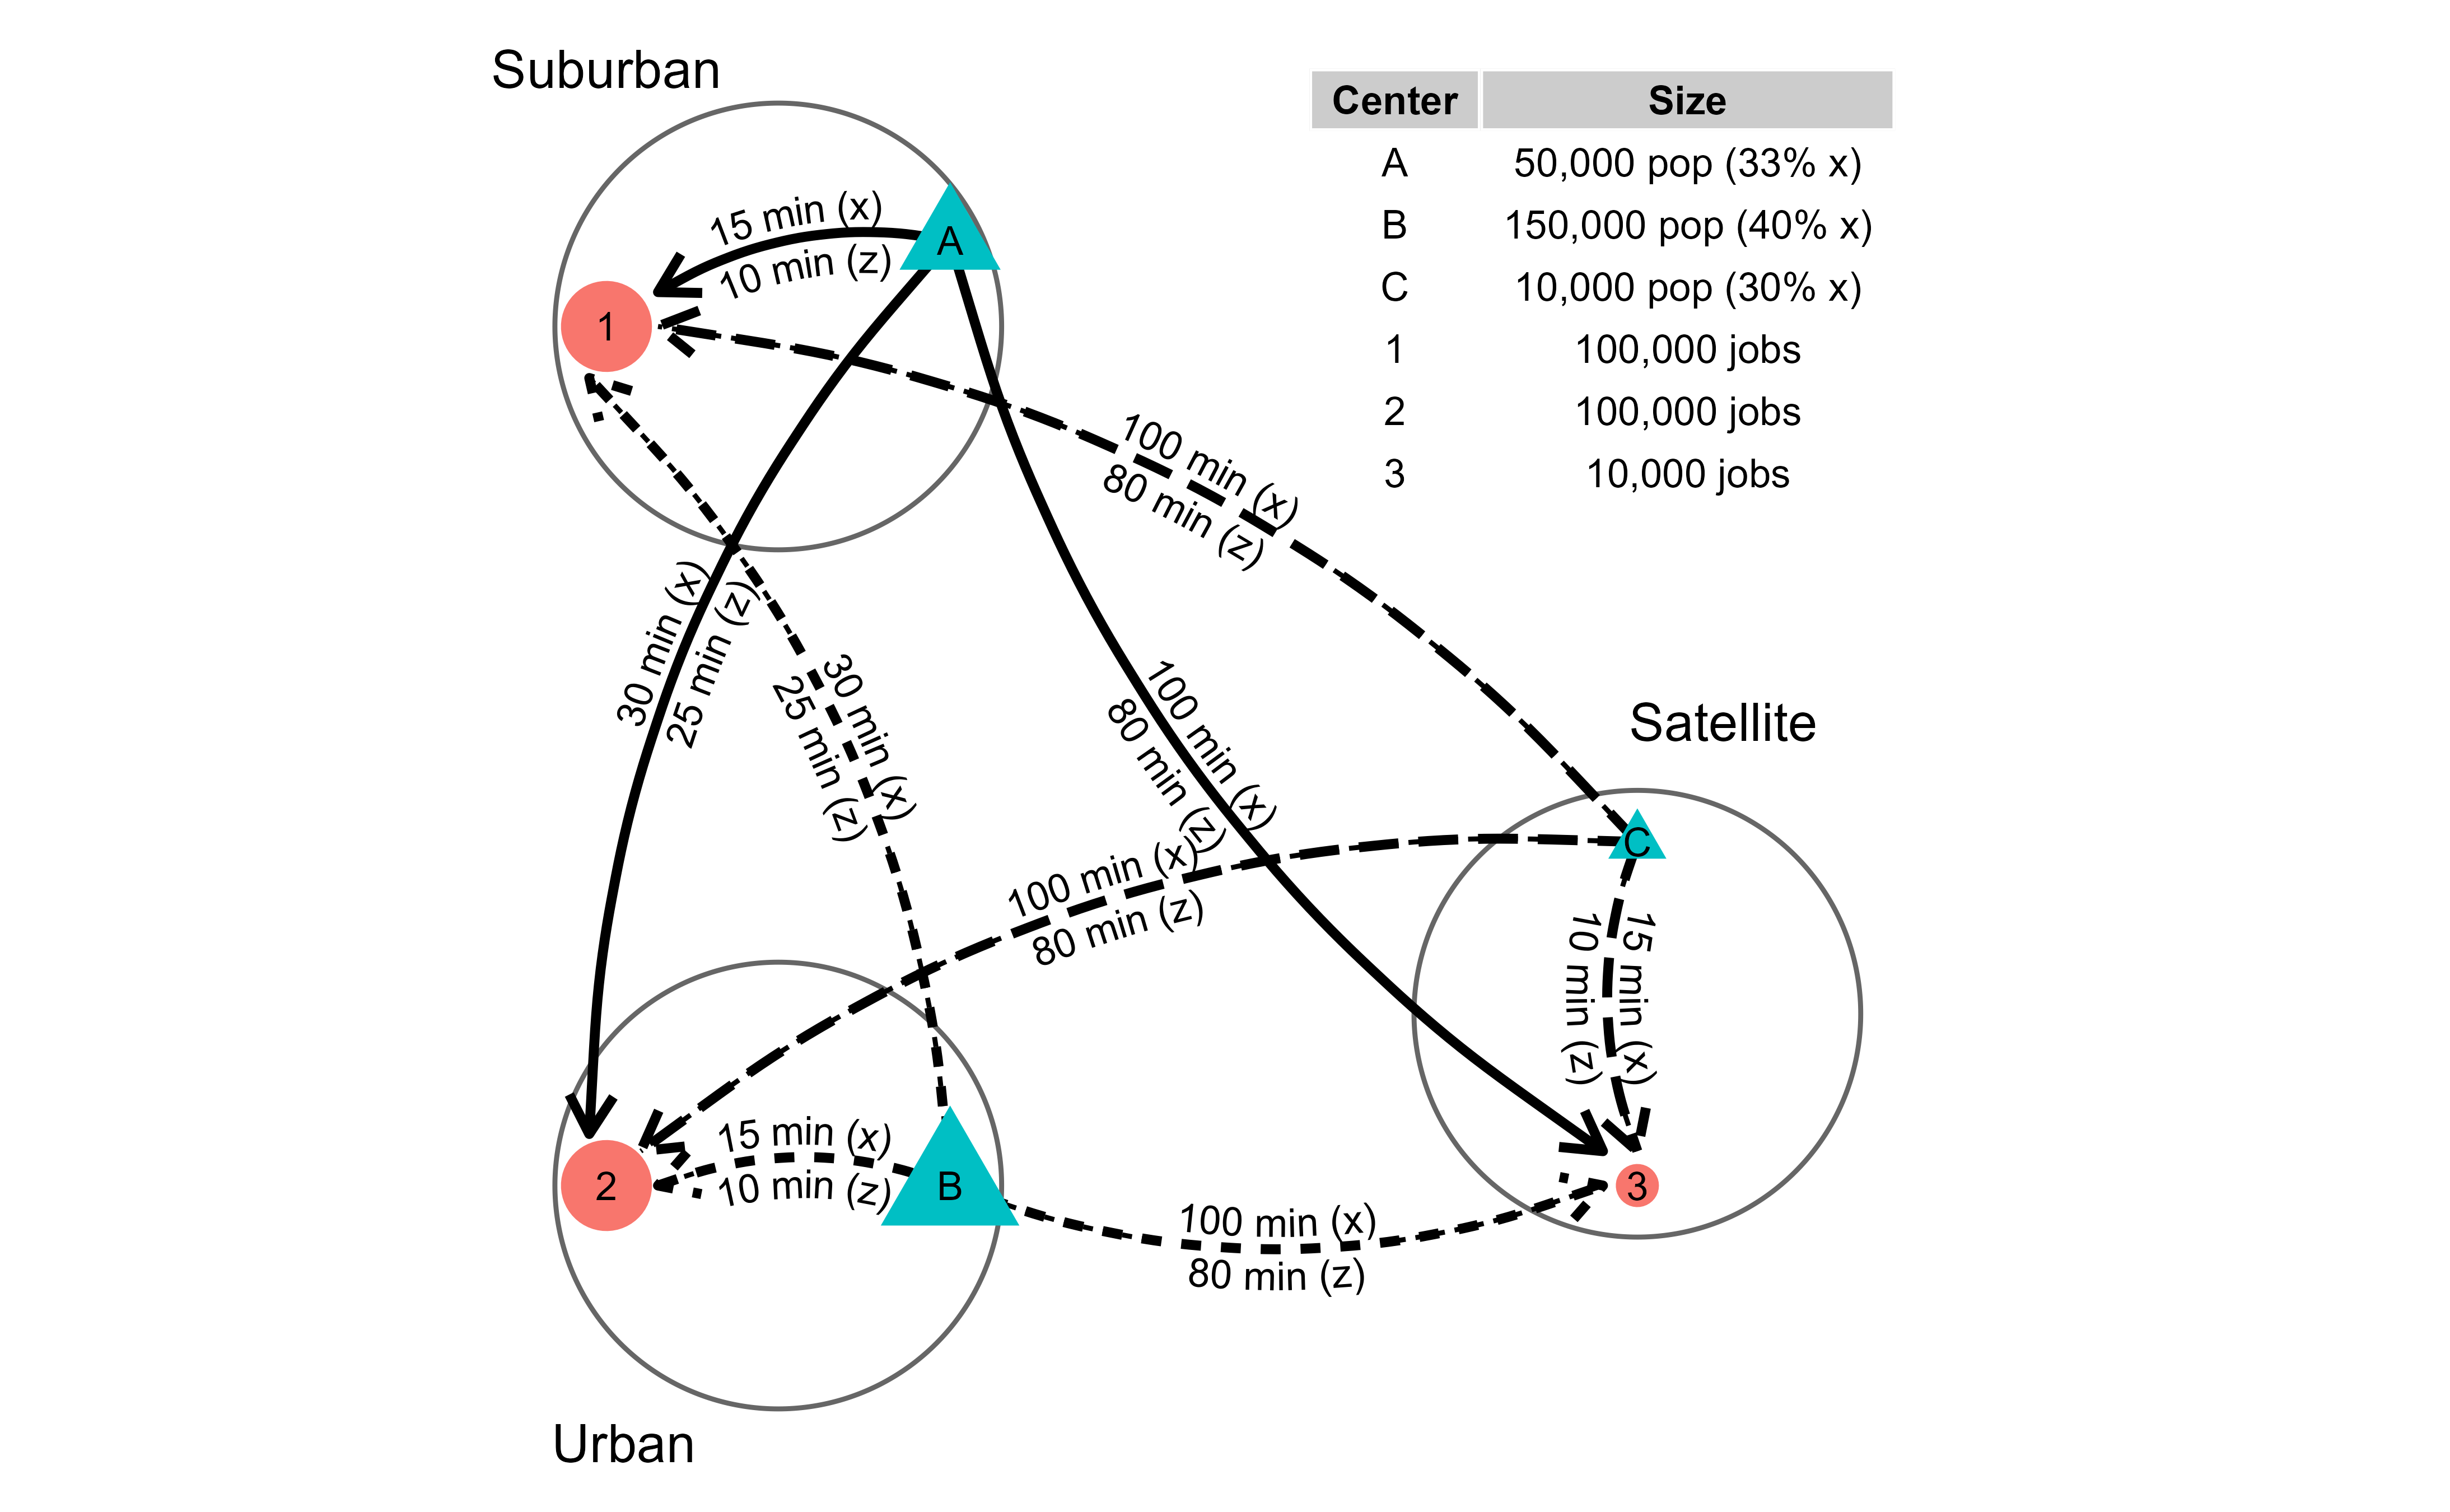
\includegraphics[width=0.85\linewidth]{images/Fig1} 

}

\caption{\label{fig:Fig1} Multimodal synthetic example: locations of employment centers (in orange), population centers (in blue), number of jobs and population, and travel times for two modes (slower mode x and faster mode z).}\label{fig:synthetic-example-plot}
\end{figure}

From the perspective of access to a \emph{finite} amount of
opportunities in the region (\(210,000\) jobs), the sub-population that
is most proximate to jobs (\DIFdelbegin \DIFdel{low }\DIFdelend \DIFaddbegin \DIFadd{lowest }\DIFaddend cost to reach), furthest from large
populations (\DIFdelbegin \DIFdel{less }\DIFdelend \DIFaddbegin \DIFadd{least }\DIFaddend competition), and uses the fastest mode \(z\)
(\DIFdelbegin \DIFdel{greater
}\DIFdelend \DIFaddbegin \DIFadd{greatest }\DIFaddend range) can potentially reach the largest number of
opportunities. This appears to be the sub-population at \(A\) using mode
\(z\). Sub-populations located in opposite conditions (i.e., more
distant from jobs, close to large populations, and using \DIFdelbegin \DIFdel{slow }\DIFdelend \DIFaddbegin \DIFadd{slower }\DIFaddend mode
\(x\)) are at a relative disadvantage. The competition for opportunities
between different mode-using populations matters as it reflects how well
the land-use and transport system serves (or does not serve) certain
populations.

\global\setlength{\Oldarrayrulewidth}{\arrayrulewidth}

\global\setlength{\Oldtabcolsep}{\tabcolsep}

\setlength{\tabcolsep}{0pt}

\renewcommand*{\arraystretch}{1.5}



\providecommand{\ascline}[3]{\noalign{\global\arrayrulewidth #1}\arrayrulecolor[HTML]{#2}\cline{#3}}

\begin{longtable}[c]{|p{0.88in}|p{0.41in}|p{1.05in}|p{0.58in}|p{1.05in}|p{0.58in}|p{1.05in}}

\caption{Accessibility\ values\ at\ each\ origin\ (i)\ per\ mode\ (m)\ (columns\ three\ to\ five)\ and\ aggregated\ per\ i\ (columns\ six\ and\ seven)\ for\ the\ synthetic\ example.}\\

\ascline{1.5pt}{666666}{1-7}

\multicolumn{1}{>{\raggedright}m{\dimexpr 0.88in+0\tabcolsep}}{\textcolor[HTML]{000000}{\fontsize{11}{11}\selectfont{i}}} & \multicolumn{1}{>{\raggedright}m{\dimexpr 0.41in+0\tabcolsep}}{\textcolor[HTML]{000000}{\fontsize{11}{11}\selectfont{m}}} & \multicolumn{1}{!{\color[HTML]{666666}\vrule width 1pt}>{\raggedleft}m{\dimexpr 1.05in+0\tabcolsep}}{\textcolor[HTML]{000000}{\fontsize{11}{11}\selectfont{S}}\textcolor[HTML]{000000}{\textsubscript{\fontsize{11}{11}\selectfont{i}}}\textcolor[HTML]{000000}{\textsuperscript{\fontsize{11}{11}\selectfont{m}}}} & \multicolumn{1}{>{\raggedleft}m{\dimexpr 0.58in+0\tabcolsep}}{\textcolor[HTML]{000000}{\fontsize{11}{11}\selectfont{a}}\textcolor[HTML]{000000}{\textsubscript{\fontsize{11}{11}\selectfont{i}}}\textcolor[HTML]{000000}{\textsuperscript{\fontsize{11}{11}\selectfont{m}}}} & \multicolumn{1}{>{\raggedleft}m{\dimexpr 1.05in+0\tabcolsep}}{\textcolor[HTML]{000000}{\fontsize{11}{11}\selectfont{V}}\textcolor[HTML]{000000}{\textsubscript{\fontsize{11}{11}\selectfont{i}}}\textcolor[HTML]{000000}{\textsuperscript{\fontsize{11}{11}\selectfont{m}}}} & \multicolumn{1}{!{\color[HTML]{666666}\vrule width 1pt}>{\raggedleft}m{\dimexpr 0.58in+0\tabcolsep}}{\textcolor[HTML]{000000}{\fontsize{11}{11}\selectfont{a}}\textcolor[HTML]{000000}{\textsubscript{\fontsize{11}{11}\selectfont{i}}}} & \multicolumn{1}{>{\raggedleft}m{\dimexpr 1.05in+0\tabcolsep}}{\textcolor[HTML]{000000}{\fontsize{11}{11}\selectfont{V}}\textcolor[HTML]{000000}{\textsubscript{\fontsize{11}{11}\selectfont{i}}}} \\

\ascline{1.5pt}{666666}{1-7}\endfirsthead \caption[]{Accessibility\ values\ at\ each\ origin\ (i)\ per\ mode\ (m)\ (columns\ three\ to\ five)\ and\ aggregated\ per\ i\ (columns\ six\ and\ seven)\ for\ the\ synthetic\ example.}\\

\ascline{1.5pt}{666666}{1-7}

\multicolumn{1}{>{\raggedright}m{\dimexpr 0.88in+0\tabcolsep}}{\textcolor[HTML]{000000}{\fontsize{11}{11}\selectfont{i}}} & \multicolumn{1}{>{\raggedright}m{\dimexpr 0.41in+0\tabcolsep}}{\textcolor[HTML]{000000}{\fontsize{11}{11}\selectfont{m}}} & \multicolumn{1}{!{\color[HTML]{666666}\vrule width 1pt}>{\raggedleft}m{\dimexpr 1.05in+0\tabcolsep}}{\textcolor[HTML]{000000}{\fontsize{11}{11}\selectfont{S}}\textcolor[HTML]{000000}{\textsubscript{\fontsize{11}{11}\selectfont{i}}}\textcolor[HTML]{000000}{\textsuperscript{\fontsize{11}{11}\selectfont{m}}}} & \multicolumn{1}{>{\raggedleft}m{\dimexpr 0.58in+0\tabcolsep}}{\textcolor[HTML]{000000}{\fontsize{11}{11}\selectfont{a}}\textcolor[HTML]{000000}{\textsubscript{\fontsize{11}{11}\selectfont{i}}}\textcolor[HTML]{000000}{\textsuperscript{\fontsize{11}{11}\selectfont{m}}}} & \multicolumn{1}{>{\raggedleft}m{\dimexpr 1.05in+0\tabcolsep}}{\textcolor[HTML]{000000}{\fontsize{11}{11}\selectfont{V}}\textcolor[HTML]{000000}{\textsubscript{\fontsize{11}{11}\selectfont{i}}}\textcolor[HTML]{000000}{\textsuperscript{\fontsize{11}{11}\selectfont{m}}}} & \multicolumn{1}{!{\color[HTML]{666666}\vrule width 1pt}>{\raggedleft}m{\dimexpr 0.58in+0\tabcolsep}}{\textcolor[HTML]{000000}{\fontsize{11}{11}\selectfont{a}}\textcolor[HTML]{000000}{\textsubscript{\fontsize{11}{11}\selectfont{i}}}} & \multicolumn{1}{>{\raggedleft}m{\dimexpr 1.05in+0\tabcolsep}}{\textcolor[HTML]{000000}{\fontsize{11}{11}\selectfont{V}}\textcolor[HTML]{000000}{\textsubscript{\fontsize{11}{11}\selectfont{i}}}} \\

\ascline{1.5pt}{666666}{1-7}\endhead



\multicolumn{1}{>{\raggedright}m{\dimexpr 0.88in+0\tabcolsep}}{} & \multicolumn{1}{>{\raggedright}m{\dimexpr 0.41in+0\tabcolsep}}{\textcolor[HTML]{000000}{\fontsize{11}{11}\selectfont{x}}} & \multicolumn{1}{!{\color[HTML]{666666}\vrule width 1pt}>{\raggedleft}m{\dimexpr 1.05in+0\tabcolsep}}{\textcolor[HTML]{000000}{\fontsize{11}{11}\selectfont{27,292.18}}} & \multicolumn{1}{>{\raggedleft}m{\dimexpr 0.58in+0\tabcolsep}}{\textcolor[HTML]{000000}{\fontsize{11}{11}\selectfont{0.95}}} & \multicolumn{1}{>{\raggedleft}m{\dimexpr 1.05in+0\tabcolsep}}{\textcolor[HTML]{000000}{\fontsize{11}{11}\selectfont{15,696.89}}} & \multicolumn{1}{!{\color[HTML]{666666}\vrule width 1pt}>{\raggedleft}m{\dimexpr 0.58in+0\tabcolsep}}{} & \multicolumn{1}{>{\raggedleft}m{\dimexpr 1.05in+0\tabcolsep}}{} \\





\multicolumn{1}{>{\raggedright}m{\dimexpr 0.88in+0\tabcolsep}}{\multirow[c]{-2}{*}{\parbox{0.88in}{\raggedright \textcolor[HTML]{000000}{\fontsize{11}{11}\selectfont{A}}}}} & \multicolumn{1}{>{\raggedright}m{\dimexpr 0.41in+0\tabcolsep}}{\textcolor[HTML]{000000}{\fontsize{11}{11}\selectfont{z}}} & \multicolumn{1}{!{\color[HTML]{666666}\vrule width 1pt}>{\raggedleft}m{\dimexpr 1.05in+0\tabcolsep}}{\textcolor[HTML]{000000}{\fontsize{11}{11}\selectfont{44,999.80}}} & \multicolumn{1}{>{\raggedleft}m{\dimexpr 0.58in+0\tabcolsep}}{\textcolor[HTML]{000000}{\fontsize{11}{11}\selectfont{1.57}}} & \multicolumn{1}{>{\raggedleft}m{\dimexpr 1.05in+0\tabcolsep}}{\textcolor[HTML]{000000}{\fontsize{11}{11}\selectfont{51,785.72}}} & \multicolumn{1}{!{\color[HTML]{666666}\vrule width 1pt}>{\raggedleft}m{\dimexpr 0.58in+0\tabcolsep}}{\multirow[c]{-2}{*}{\parbox{0.58in}{\raggedleft \textcolor[HTML]{000000}{\fontsize{11}{11}\selectfont{1.36}}}}} & \multicolumn{1}{>{\raggedleft}m{\dimexpr 1.05in+0\tabcolsep}}{\multirow[c]{-2}{*}{\parbox{1.05in}{\raggedleft \textcolor[HTML]{000000}{\fontsize{11}{11}\selectfont{67,482.61}}}}} \\

\ascline{1pt}{666666}{1-7}



\multicolumn{1}{>{\raggedright}m{\dimexpr 0.88in+0\tabcolsep}}{} & \multicolumn{1}{>{\raggedright}m{\dimexpr 0.41in+0\tabcolsep}}{\textcolor[HTML]{000000}{\fontsize{11}{11}\selectfont{x}}} & \multicolumn{1}{!{\color[HTML]{666666}\vrule width 1pt}>{\raggedleft}m{\dimexpr 1.05in+0\tabcolsep}}{\textcolor[HTML]{000000}{\fontsize{11}{11}\selectfont{27,292.18}}} & \multicolumn{1}{>{\raggedleft}m{\dimexpr 0.58in+0\tabcolsep}}{\textcolor[HTML]{000000}{\fontsize{11}{11}\selectfont{0.64}}} & \multicolumn{1}{>{\raggedleft}m{\dimexpr 1.05in+0\tabcolsep}}{\textcolor[HTML]{000000}{\fontsize{11}{11}\selectfont{38,170.03}}} & \multicolumn{1}{!{\color[HTML]{666666}\vrule width 1pt}>{\raggedleft}m{\dimexpr 0.58in+0\tabcolsep}}{} & \multicolumn{1}{>{\raggedleft}m{\dimexpr 1.05in+0\tabcolsep}}{} \\





\multicolumn{1}{>{\raggedright}m{\dimexpr 0.88in+0\tabcolsep}}{\multirow[c]{-2}{*}{\parbox{0.88in}{\raggedright \textcolor[HTML]{000000}{\fontsize{11}{11}\selectfont{B}}}}} & \multicolumn{1}{>{\raggedright}m{\dimexpr 0.41in+0\tabcolsep}}{\textcolor[HTML]{000000}{\fontsize{11}{11}\selectfont{z}}} & \multicolumn{1}{!{\color[HTML]{666666}\vrule width 1pt}>{\raggedleft}m{\dimexpr 1.05in+0\tabcolsep}}{\textcolor[HTML]{000000}{\fontsize{11}{11}\selectfont{44,999.80}}} & \multicolumn{1}{>{\raggedleft}m{\dimexpr 0.58in+0\tabcolsep}}{\textcolor[HTML]{000000}{\fontsize{11}{11}\selectfont{1.05}}} & \multicolumn{1}{>{\raggedleft}m{\dimexpr 1.05in+0\tabcolsep}}{\textcolor[HTML]{000000}{\fontsize{11}{11}\selectfont{94,468.91}}} & \multicolumn{1}{!{\color[HTML]{666666}\vrule width 1pt}>{\raggedleft}m{\dimexpr 0.58in+0\tabcolsep}}{\multirow[c]{-2}{*}{\parbox{0.58in}{\raggedleft \textcolor[HTML]{000000}{\fontsize{11}{11}\selectfont{0.88}}}}} & \multicolumn{1}{>{\raggedleft}m{\dimexpr 1.05in+0\tabcolsep}}{\multirow[c]{-2}{*}{\parbox{1.05in}{\raggedleft \textcolor[HTML]{000000}{\fontsize{11}{11}\selectfont{132,638.94}}}}} \\

\ascline{1pt}{666666}{1-7}



\multicolumn{1}{>{\raggedright}m{\dimexpr 0.88in+0\tabcolsep}}{} & \multicolumn{1}{>{\raggedright}m{\dimexpr 0.41in+0\tabcolsep}}{\textcolor[HTML]{000000}{\fontsize{11}{11}\selectfont{x}}} & \multicolumn{1}{!{\color[HTML]{666666}\vrule width 1pt}>{\raggedleft}m{\dimexpr 1.05in+0\tabcolsep}}{\textcolor[HTML]{000000}{\fontsize{11}{11}\selectfont{2,240.38}}} & \multicolumn{1}{>{\raggedleft}m{\dimexpr 0.58in+0\tabcolsep}}{\textcolor[HTML]{000000}{\fontsize{11}{11}\selectfont{0.68}}} & \multicolumn{1}{>{\raggedleft}m{\dimexpr 1.05in+0\tabcolsep}}{\textcolor[HTML]{000000}{\fontsize{11}{11}\selectfont{2,035.86}}} & \multicolumn{1}{!{\color[HTML]{666666}\vrule width 1pt}>{\raggedleft}m{\dimexpr 0.58in+0\tabcolsep}}{} & \multicolumn{1}{>{\raggedleft}m{\dimexpr 1.05in+0\tabcolsep}}{} \\





\multicolumn{1}{>{\raggedright}m{\dimexpr 0.88in+0\tabcolsep}}{\multirow[c]{-2}{*}{\parbox{0.88in}{\raggedright \textcolor[HTML]{000000}{\fontsize{11}{11}\selectfont{C}}}}} & \multicolumn{1}{>{\raggedright}m{\dimexpr 0.41in+0\tabcolsep}}{\textcolor[HTML]{000000}{\fontsize{11}{11}\selectfont{z}}} & \multicolumn{1}{!{\color[HTML]{666666}\vrule width 1pt}>{\raggedleft}m{\dimexpr 1.05in+0\tabcolsep}}{\textcolor[HTML]{000000}{\fontsize{11}{11}\selectfont{3,745.89}}} & \multicolumn{1}{>{\raggedleft}m{\dimexpr 0.58in+0\tabcolsep}}{\textcolor[HTML]{000000}{\fontsize{11}{11}\selectfont{1.12}}} & \multicolumn{1}{>{\raggedleft}m{\dimexpr 1.05in+0\tabcolsep}}{\textcolor[HTML]{000000}{\fontsize{11}{11}\selectfont{7,842.59}}} & \multicolumn{1}{!{\color[HTML]{666666}\vrule width 1pt}>{\raggedleft}m{\dimexpr 0.58in+0\tabcolsep}}{\multirow[c]{-2}{*}{\parbox{0.58in}{\raggedleft \textcolor[HTML]{000000}{\fontsize{11}{11}\selectfont{0.99}}}}} & \multicolumn{1}{>{\raggedleft}m{\dimexpr 1.05in+0\tabcolsep}}{\multirow[c]{-2}{*}{\parbox{1.05in}{\raggedleft \textcolor[HTML]{000000}{\fontsize{11}{11}\selectfont{9,878.45}}}}} \\

\ascline{1pt}{666666}{1-7}



\multicolumn{1}{>{\raggedright}m{\dimexpr 0.88in+0\tabcolsep}}{\textcolor[HTML]{000000}{\fontsize{11}{11}\selectfont{TOTALS}}} & \multicolumn{1}{>{\raggedright}m{\dimexpr 0.41in+0\tabcolsep}}{\textcolor[HTML]{000000}{\fontsize{11}{11}\selectfont{}}} & \multicolumn{1}{!{\color[HTML]{666666}\vrule width 1pt}>{\raggedleft}m{\dimexpr 1.05in+0\tabcolsep}}{\textcolor[HTML]{000000}{\fontsize{11}{11}\selectfont{150,570.22}}} & \multicolumn{1}{>{\raggedleft}m{\dimexpr 0.58in+0\tabcolsep}}{\textcolor[HTML]{000000}{\fontsize{11}{11}\selectfont{N/A}}} & \multicolumn{1}{>{\raggedleft}m{\dimexpr 1.05in+0\tabcolsep}}{\textcolor[HTML]{000000}{\fontsize{11}{11}\selectfont{210,000.00}}} & \multicolumn{1}{!{\color[HTML]{666666}\vrule width 1pt}>{\raggedleft}m{\dimexpr 0.58in+0\tabcolsep}}{\textcolor[HTML]{000000}{\fontsize{11}{11}\selectfont{N/A}}} & \multicolumn{1}{>{\raggedleft}m{\dimexpr 1.05in+0\tabcolsep}}{\textcolor[HTML]{000000}{\fontsize{11}{11}\selectfont{210,000.00}}} \\

\ascline{1.5pt}{666666}{1-7}



\end{longtable}



\arrayrulecolor[HTML]{000000}

\global\setlength{\arrayrulewidth}{\Oldarrayrulewidth}

\global\setlength{\tabcolsep}{\Oldtabcolsep}

\renewcommand*{\arraystretch}{1}

The values calculated for \(S_i^m\) (Hansen-type accessibility),
\(a_i^m\) (Shen-type accessibility), and \(V_i^m\) (spatial
availability) for each \(i\) and \(m\) are shown in the middle three
columns and are aggregated for each \(i\) in the final two columns in
Table 1 . As in the example in Shen \DIFaddbegin \DIFadd{(1998) }\DIFaddend {[}\DIFdelbegin \DIFdel{12}\DIFdelend \DIFaddbegin \DIFadd{24}\DIFaddend {]}, we use a negative
exponential impedance function
\(f^m(c_{ij}^m) = \exp(-\beta\cdot c_{ij})\) with \(\beta=0.1\) for both
\(x\) and \(z\) modes for all accessibility measures calculations.
Notice that in this example we use the same impedance function but the
travel times are different for the two modes. More generally, it is
possible to use different impedance functions for the modes, as \DIFdelbegin \DIFdel{demonstrated in }\DIFdelend the
empirical example in the following section \DIFaddbegin \DIFadd{demonstrates}\DIFaddend .

Hansen-type accessibility \(S_i^m\) is presented for each origin and
mode in the third column of Table 1 . For all \(i\), the travel by \(z\)
results in higher values of \(S_i^m\) than travel by \(x\). Lack of
competition, or alternatively the assumption of an inexhaustible
resource in the calculation of \(S_i^m\), \DIFdelbegin \DIFdel{lead }\DIFdelend \DIFaddbegin \DIFadd{leds }\DIFaddend to a curious result.
Since the populations in \(A\) and \(B\) have the same travel impedance
to employment centers \(1\), \(2\) and \(3\) (either 15, 30, or 100
minutes using \(x\) or 10, 25, or 80 minutes using \(z\)), their values
of \(S_i^m\) are the same for both \(A\) and \(B\). Furthermore, the
total sum of \(S_i^m\) in the region is equal to 150,570.2. This value
lacks an intuitive interpretation: it represents the weighted sum of
opportunities that may be reached within the region according to the
travel impedance (i.e., the travel behavior and the characteristics of
the modes) and does not usefully translate into any sort of benchmark.
To connect this example to the aforementioned literature, \(S_i^m\) is
calculated in the work of Tahmasbi et al.\DIFaddbegin \DIFadd{~(2019) }\DIFaddend {[}\DIFdelbegin \DIFdel{21}\DIFdelend \DIFaddbegin \DIFadd{34}\DIFaddend {]}; they contrast
differences in \(S_i^m\) values between modes in a relative and
comparative sense, but make no further interpretation of the \(S_i^m\)
values. More densely populated metropolitan regions will tend to have
more opportunities and hence large \(S_i^m\) values and less densely
regions, smaller values; how much of these differences may simply an
artifact of region density?

In the fourth and sixth columns in Table 1 the results for Shen-type
accessibility are reported: first for both origin and mode \(a_i^m\) as
well as aggregated by the weighted mean mode-population (
\(\sum_m \frac{P_i^m}{P_i}*a_i^m\) ) to represent a value for each
origin \(a_i\). Unlike \(S_i^m\), this measure does considers
\emph{competition}. For instance, the population travelling by \(x\)
from \(A\) and \(B\) do not have the same values of \(a_i^m\) as those
travelling by \(z\). In fact, \(A\) has the highest values \(a_i^m\) and
\(a_i\) values since this center has the lowest travel impedance to
opportunities (lower than at \(C\), \(A\) and \(B\) are equal) and faces
relatively low competition, not being close to a relatively large
population (lower than at \(B\)).

However, the calculations of \(a_i^m\) are not constrained: the total
sum of \(a_i^m\) or \(a_i\) is practically meaningless since it
represents a sum of ratios. For instance, the population travelling by
\(z\) from \(A\) has a value of 1.57 jobs per job-seeking population
compared to 0.95 for users of mode \(x\). What is the meaning of these
values? The difference between these modes is equal to 0.62, but 0.62 of
what? How many more job opportunities can users of \(z\) reach compared
to user of \(x\)? When \(a_i^m\) is aggregated to \(a_i\) as shown in
the sixth column, the values face similar interpretability issues. The
Shen-type measure is implemented in aforementioned work of Tao et
al.\DIFaddbegin \DIFadd{~(2020) }\DIFaddend {[}\DIFdelbegin \DIFdel{36}\DIFdelend \DIFaddbegin \DIFadd{48}\DIFaddend {]} to calculate modal \(a_i^m\) values and the
aggregated \(a_i\) is implemented in the work of Carpentier et
al.\DIFaddbegin \DIFadd{~(2020) }\DIFaddend {[}\DIFdelbegin \DIFdel{38}\DIFdelend \DIFaddbegin \DIFadd{50}\DIFaddend {]}. However, similar to Hansen-type accessibility,
these works discuss relative and spatially comparative differences in
values, but veer from interpreting the values of \(a_i^m\) or \(a_i\)
themselves. In fairness, interpretation is complicated by the multiple
counting of opportunities between zones and modes.

In contrast, spatial availability \(V_i\) considers competition and is
constrained such that the total sum of values is equal to the total
number of opportunities in the region (i.e., \(210,000\) jobs). Seen in
fifth column of Table 1 , the values of \(V_i^m\) \DIFdelbegin \DIFdel{in }\DIFdelend \DIFaddbegin \DIFadd{for }\DIFaddend \(A\) and \(B\)
are not the same within each mode (as this measure considers
competition). In fact, at \(A\), users of mode \(z\) capture 36,088.84
more spatially available jobs (of the \(210,000\) jobs in the region)
than the sub-population travelling by \DIFaddbegin \DIFadd{the slower-mode }\DIFaddend \(x\). The
numerical difference is clear since it refers to opportunities out of
the total.

Furthermore, the proportional allocation mechanism also means that the
values of \(V_i^m\) for any origin \(i\) can be aggregated across \(m\)
and compared between zones (\(V_i = \sum_m{\sum_i{V_i^m}}\)). This
aggregation, \(V_i\), is shown in the seventh column in Table 1 . \DIFdelbegin \DIFdel{Again
looking at center }\DIFdelend \(A\)
\DIFdelbegin \DIFdel{, \(A\) }\DIFdelend is allocated 67,482.61 spatially available opportunities for both modes.
77\% of this spatial availability allocated to \(A\) is assigned to
users of mode \(z\) despite representing 66\% of \(A\)'s population.

Spatial availability can be further aggregated to better interpret
competition between modes. Across the entire region, 130,000 people use
\(z\) (62\% of the region population). However, users of \(z\) account
for 73\% of the region's total spatial availability - while the
remaining 27\% is allocated to users of mode \(x\) who are 38\% of the
total population. Notably, the population who uses \(x\) have 11\% fewer
spatially available opportunities than its share in the population. This
realization \DIFdelbegin \DIFdel{leads }\DIFdelend \DIFaddbegin \DIFadd{could lead }\DIFaddend us to ask normative questions\DIFdelbegin \DIFdel{such as, }\DIFdelend \DIFaddbegin \DIFadd{: }\DIFaddend how unequal should
availability of opportunities be by mode? What intervention could help
to redistribute spatial availability to sub-populations commensurate
with their proportion of the total?

Since spatial availability is constrained \DIFdelbegin \DIFdel{and has an interpretable
meaning as a proportion of }\DIFdelend \DIFaddbegin \DIFadd{to }\DIFaddend the total opportunities in
the region, the values at \(i\) have a straighforward interpretation.
Inequality in \(V_i^m\) values can be explored through a variety of
approaches. For instance, consider travel times. The population of
travelers who use \(z\) accounts for 67\% of the potential travel time
traveled in the region: this is 7\% less travel time than the proportion
of spatial available opportunities that is allocated to them. In other
words, the population of users of \(z\) travels fewer minutes overall
and has more spatial availability of opportunities than users of the
slower mode \(x\).

Alternatively, inequities in spatial availability between modes can be
explored through proportional benchmarks. A spatial availability per
capita \(v_i^m\) is presented in Equation (\ref{eq:SA-per-capita}):

\begin{equation}
\label{eq:SA-per-capita}
v_{i}^m = \frac{V_{i}^m}{P_{i}^m}
\end{equation}

The values of \(v_i^m\) for \(A\), \(B\), and \(C\) for users of \(x\)
are 0.95, 0.64 and 0.68 spatially available jobs per capita,
respectively. The values of \(v_i^m\) for users of \(z\) are much
higher, with values of: 1.57, 1.05 and 1.12 respectively. Users of
\(x\), especially those at \(B\) and \(C\), are directly impacted by the
jobs that are spatially available to users of \(z\) \emph{in addition
to} the mass effect (occurring at \(B\), high population density) and
high travel impedance (occurring at the Satellite \(C\)). \DIFaddbegin \DIFadd{Notably,
\(v_i^m\) values are equal to the ratios of the Shen-type measure
\(a_i^m\) in this case, however they take on a different interpretation.
}\DIFaddend 

If, let us say, the planning goal was to have one spatially available
job per mode-using population, a policy intervention could be devised,
to reduce the values of \(v_i^z\) (making it slower or more expensive)
and increase \DIFdelbegin \DIFdel{he }\DIFdelend \DIFaddbegin \DIFadd{the }\DIFaddend values of \(v_i^x\) (making it faster or \DIFdelbegin \DIFdel{les }\DIFdelend \DIFaddbegin \DIFadd{less
}\DIFaddend expensive). The purpose of this \DIFdelbegin \DIFdel{simple }\DIFdelend \DIFaddbegin \DIFadd{synthetic }\DIFaddend demonstration is to show how
spatial availability can be used to quantify the competitive
(dis)advantage in a multimodal application. In what follows, we
demonstrate the use of multimodal spatial availability through an
empirical example.

\hypertarget{empirical-example}{%
\section{Empirical example}\label{empirical-example}}

\hypertarget{context}{%
\subsection{Context}\label{context}}

The context for the empirical example is \DIFaddbegin \DIFadd{the city of }\DIFaddend Madrid, Spain. This
city implemented a Low Emission Zone (LEZ) in 2017 to \DIFdelbegin \DIFdel{: }\DIFdelend pursue goals set
out in the national climate change agenda \DIFdelbegin \DIFdel{, cut }\DIFdelend \DIFaddbegin \DIFadd{such as cutting }\DIFaddend nitrogen
dioxide levels \DIFdelbegin \DIFdel{, and to prioritize }\DIFdelend \DIFaddbegin \DIFadd{and prioritizing }\DIFaddend people's movement in the city. LEZs
elsewhere have similarly been implemented as interventions to reduce GHG
emissions, improve air quality, and support sustainable mobility
{[}\DIFdelbegin \DIFdel{39,40}\DIFdelend \DIFaddbegin \DIFadd{51,52}\DIFaddend {]}. Though the rules of exclusion vary by city, LEZs aim to
deter/reduce traffic in designated zones under threat of penalty (e.g.,
fines, seizure of vehicle). In other words, LEZs implement a form of
\emph{geographic discrimination} as they change how people can reach
opportunities by making it more costly for some forms of travel,
typically cars, to circulate in predetermined zones. When considering
opportunities as finite in a region, this discrimination reduces the
competition of one mode and opens up opportunities for other modes to
better thrive. At their core, LEZs operate by changing the accessibility
landscape of a city from the perspective of multiple modes.

In geographic scope, the 2017 boundaries of the LEZ in Madrid were
relatively modest, covering only approximately 4.72
km\textsuperscript{2} of the central business district of the city (the
so-called LEZ Centro). As of this writing, there are plans to expand
these boundaries to the area inside the M-30, an orbital highway in
proximity to the city center\DIFdelbegin \DIFdel{(i.e., LEZ M-30)}\DIFdelend . Within the 2017 LEZ Centro implementation,
all cars, motorcycles and freight vehicles with environmental labels A
or B (older makes and models of fossil fuel internal combustion engine
vehicles), were disallowed from entering the zone unless they are used
by residents or meet other exemptions. This restriction impacted
approximately half of all car trips that used to travel into what is now
the LEZ Centro {[}\DIFdelbegin \DIFdel{41}\DIFdelend \DIFaddbegin \DIFadd{53}\DIFaddend {]}.

\DIFdelbegin \DIFdel{For this case study, we use }\DIFdelend \DIFaddbegin \DIFadd{The purpose of this empirical example is to quantify }\DIFaddend spatial
availability to \DIFdelbegin \DIFdel{quantify access to
}\DIFdelend \DIFaddbegin \DIFadd{employment }\DIFaddend opportunities by different modes in Madrid
\DIFaddbegin \DIFadd{after LEZ Centro implementation}\DIFaddend . Particularly, we demonstrate how
\(V_i^m\) can be used to \DIFdelbegin \DIFdel{derive insights into how the restriction of
car mobility in areas around}\DIFdelend \DIFaddbegin \DIFadd{illustrate the spatial availability advantage
that more sustainable modes (that are often slower than car) gain
within}\DIFaddend /\DIFdelbegin \DIFdel{within the LEZ Centro may have allowed more sustainable (but often slower or more costly modes) to become more
competitive
}\DIFdelend \DIFaddbegin \DIFadd{around the LEZ Centro. We speculate on how this competitive
advantage is heightened as a result of the LEZ implementation that
restricts car mobility}\DIFaddend .

\begin{figure}

{\centering 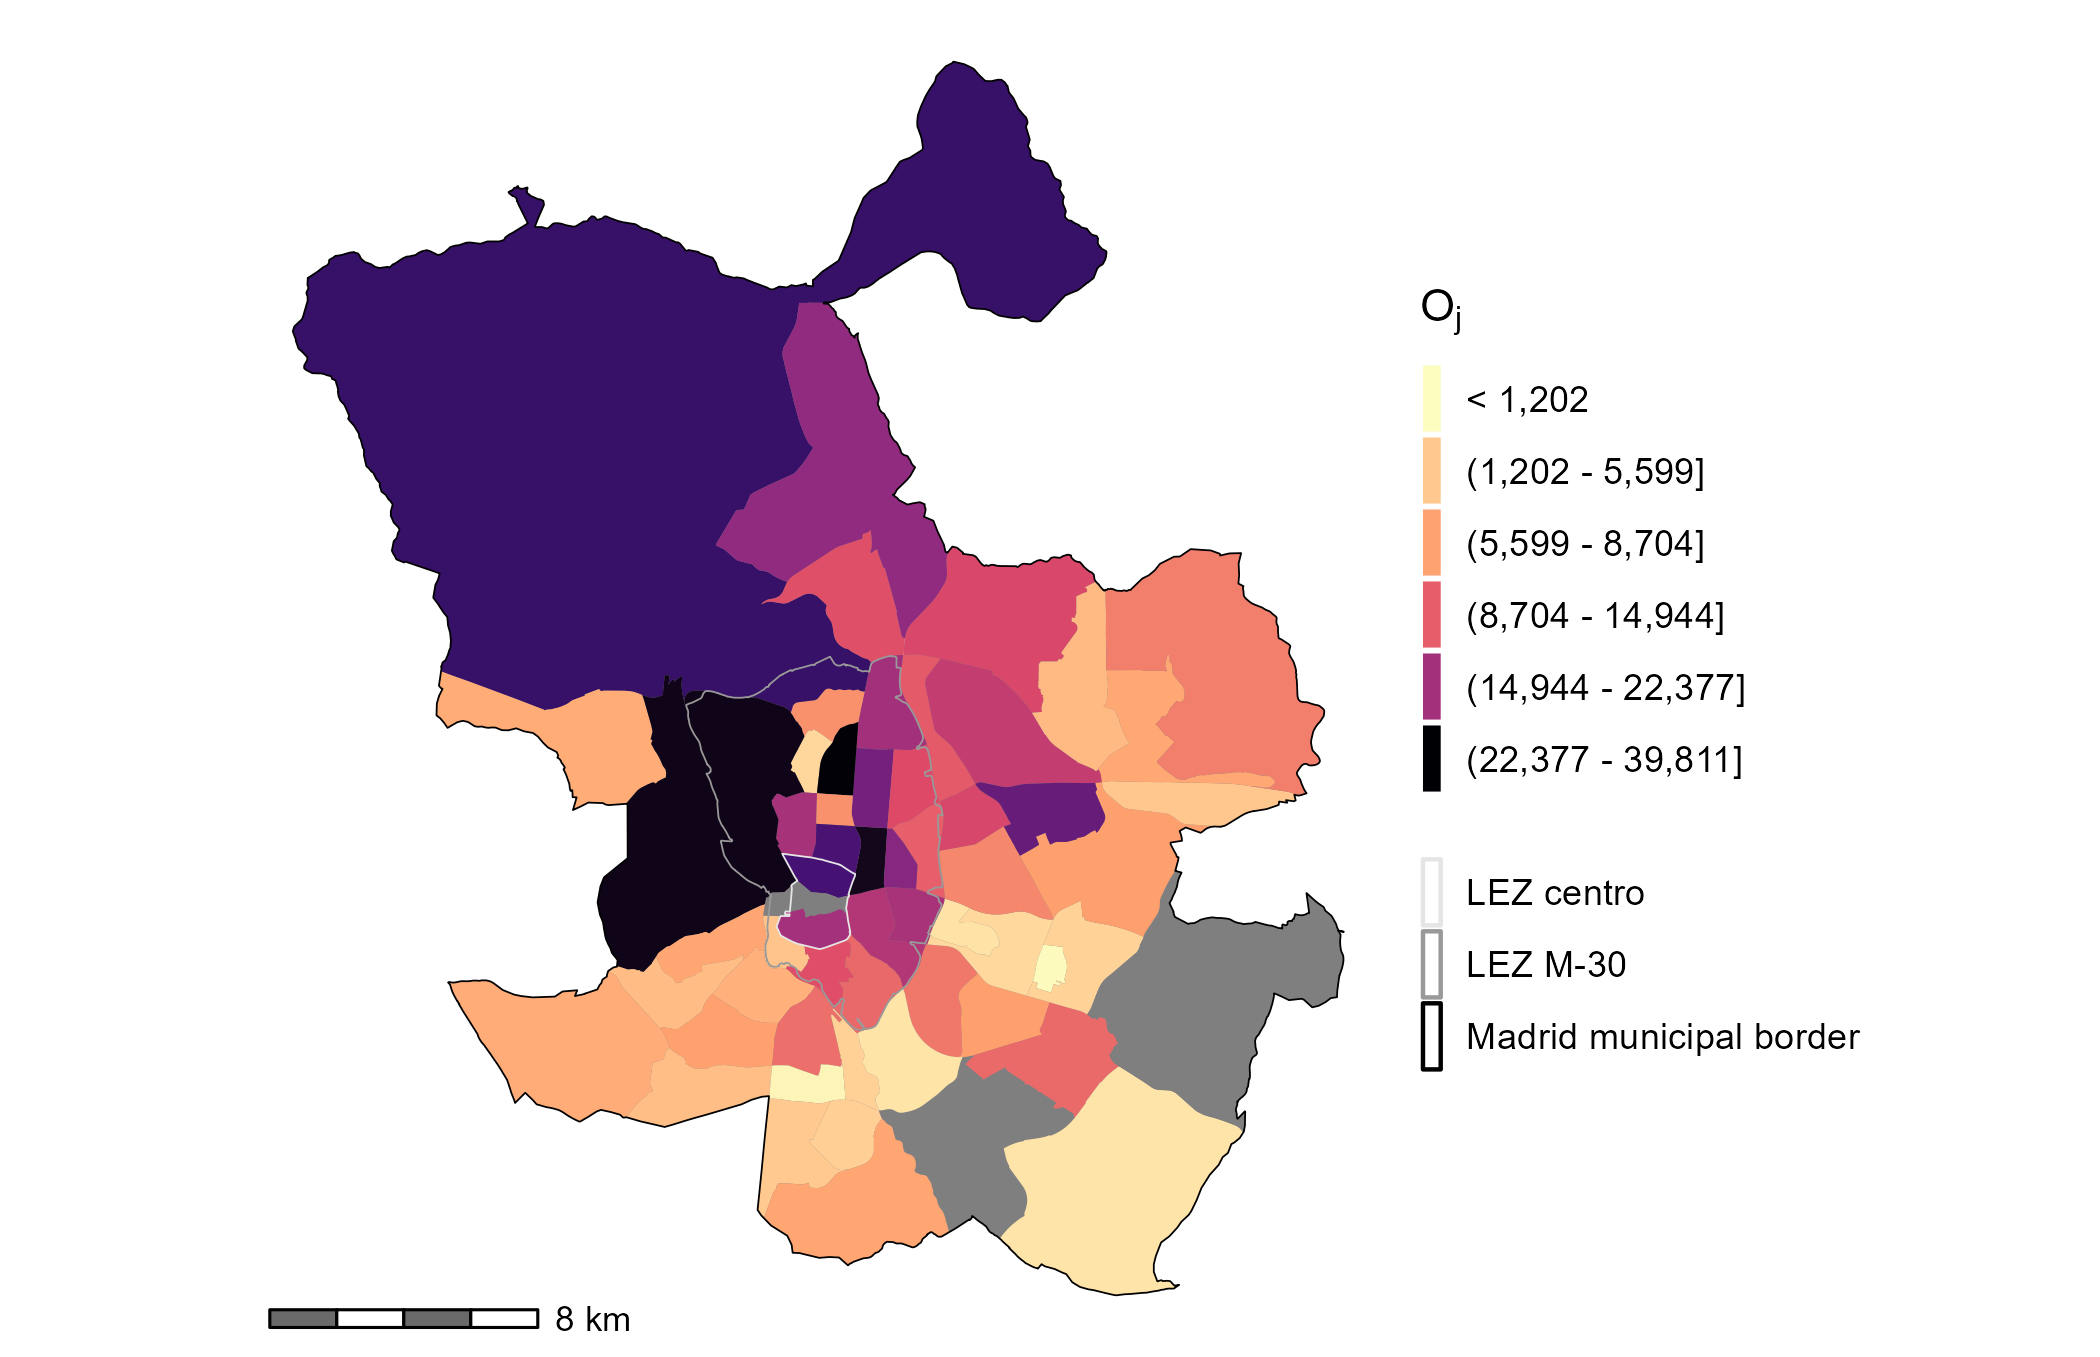
\includegraphics[width=0.85\linewidth]{images/Fig2} 

}

\caption{\label{fig:Fig2} Distribution of jobs taken by people living and working in Madrid as reported in the 2018 travel survey. Grey TAZs have no jobs. Ranges of values in the legend are quintiles. The TAZ shapefile is available from the Community of Madrid open data portal.}\label{fig:jobs-plot}
\end{figure}

\begin{figure}

{\centering 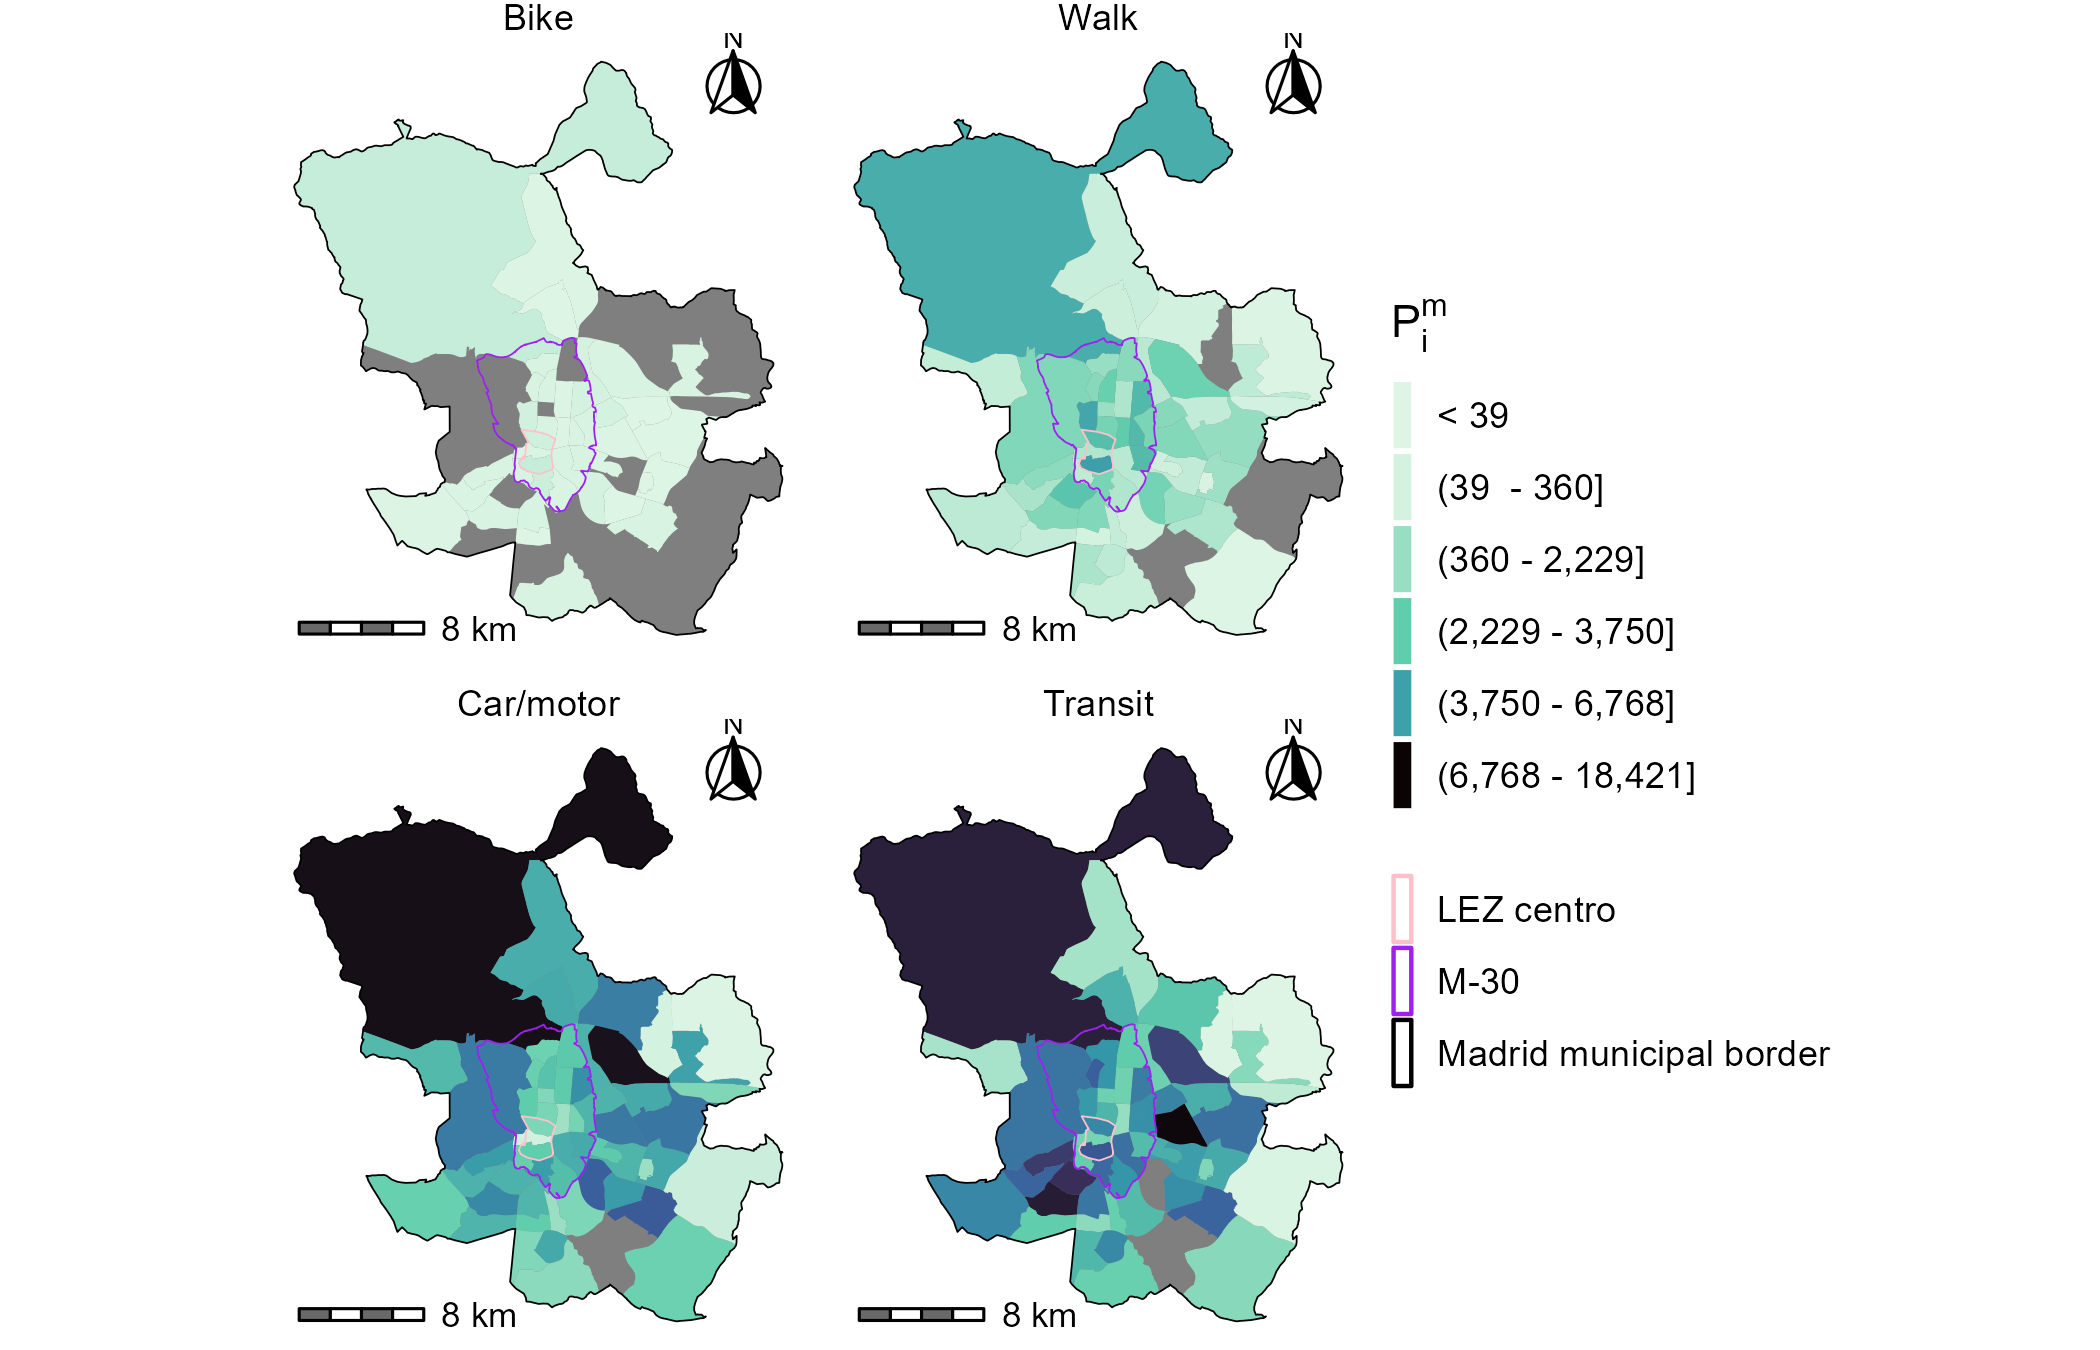
\includegraphics[width=0.85\linewidth]{images/Fig3} 

}

\caption{\label{fig:Fig3} Population living and working in Madrid by mode of transportation as reported in the 2018 travel survey and represented at the level of TAZ. Grey TAZ have no population. Ranges of values in the legend are quintiles. The TAZ shapefile is available from the Community of Madrid open data portal.}\label{fig:pop-plot}
\end{figure}

\hypertarget{data}{%
\subsection{Data}\label{data}}

The source of \DIFaddbegin \DIFadd{origin-destination }\DIFaddend data for our empirical example is the
2018 Travel Survey of the Community of Madrid {[}\DIFdelbegin \DIFdel{42}\DIFdelend \DIFaddbegin \DIFadd{54}\DIFaddend {]}. This is a
representative survey that offers a snap-shot of travel patterns for a
typical weekday in 2018. The survey collected 222,744 trips from a
representative sample of 85,064 households across the traffic analysis
zones (TAZ) in the Community of Madrid. For context, the population
older than 3 years in the Community is 6,507,184.

In this example, we use all \DIFaddbegin \DIFadd{direct }\DIFaddend home-to-full-time-work trips, by all
modes. The trips are expanded using population weights. Figures
\ref{fig:Fig2} and \ref{fig:Fig3} show the number of workers and the
distribution of full-time jobs in the City of Madrid by TAZ. The TAZ
shapefiles are available from the Community of Madrid open data portal
{[}\DIFdelbegin \DIFdel{43}\DIFdelend \DIFaddbegin \DIFadd{55}\DIFaddend {]}. The \DIFdelbegin \DIFdel{light grey }\DIFdelend \DIFaddbegin \DIFadd{pink }\DIFaddend boundary represents the LEZ Centro in effect in \DIFdelbegin \DIFdel{2017. The
survey was conducted after the introduction of LEZ Centro. The dark grey
}\DIFdelend \DIFaddbegin \DIFadd{2017
and reflected in the 2018 travel survey. The purple }\DIFaddend boundary represents
the LEZ planned for the boundaries of the M-30 highway and is present in
the plots as a spatial reference for areas in proximity to the LEZ
Centro.

The total sum of jobs \(O_j\) are shown in Figure \ref{fig:Fig2} and the
populations that go to a work destination by four modal categories
\(P^m_i\), is displayed in Figure \ref{fig:Fig3}. The modal shares in
Figure \ref{fig:Fig3} are calculated based on \DIFdelbegin \DIFdel{those measured }\DIFdelend \DIFaddbegin \DIFadd{the primary mode specified
}\DIFaddend in the survey \DIFdelbegin \DIFdel{. The modal categories and the mode types within each category are
reported }\DIFdelend \DIFaddbegin \DIFadd{and summarized into four categories }\DIFaddend as follows:

\begin{itemize}
\tightlist
\item
  Car/motor: all cars and operating modes (e.g., cab, private driver,
  company, rental car, main driver of a private car, passenger in a
  private car) and all public, private or company motorcycle/mopeds.
\item
  Transit: all bus, trams, and trains.
\item
  Bike: all bicycle trips (e.g., private, public, or company bike trips)
  and ``other'' types of micromobility options.
\item
  Walk: \DIFdelbegin \DIFdel{walking or by foot}\DIFdelend \DIFaddbegin \DIFadd{pedestrian mode}\DIFaddend .
\end{itemize}

Some aggregation of modes is necessary to calculate the travel impedance
functions by mode. From Figure \ref{fig:Fig2}, \DIFdelbegin \DIFdel{it can be seen that }\DIFdelend the largest concentration
of jobs is within, near, and to the north of LEZ Centro. The populations
with access to those jobs by mode (Figure \ref{fig:Fig3}) are spatially
distinct. Travel by car and transit represent 37\% and 47\% of the modal
share respectively. The population that travels by transit is more
spatially distributed than those using cars - particularly near and
within LEZ Centro. This distribution is likely caused by a variety of
factors including: transit coverage and service within with city,
effective car infrastructure outside of the M-30, and/or the impact of
the LEZ Centro itself. From Figure \ref{fig:Fig3}, \DIFdelbegin \DIFdel{it can be seen that }\DIFdelend active travel is less
common than motorised trips at 1\% and 15\% for cycling and walking
respectively. Noticeably, there is a positive trend between the walking
and cycling in zones where transit is also present. This positive trend
is higher than for \DIFdelbegin \DIFdel{car trip }\DIFdelend \DIFaddbegin \DIFadd{car-using }\DIFaddend populations.

Travel times are provided within the travel survey by mode. This
information is used to calibrate mode-specific travel impedance
functions \(f^m(c_{ij}^m)\). To illustrate the modal differences in
travel times, the following descriptive statistics per mode are
presented:

\begin{itemize}
\tightlist
\item
  Car/motor: mean 36 minutes (min: 0 minutes, Q2: 15 minutes, Q3: 55
  minutes, max: 120 minutes)
\item
  Transit: mean 55 minutes (min: 1 minutes, Q2: 30 minutes, Q3: 80
  minutes, max: 120 minutes)
\item
  Bike: mean 34 minutes (min: 5 minutes, Q2: 15 minutes, Q3: 40 minutes,
  max: 115 minutes)
\item
  Walk: mean 27 minutes (min: 1 minutes, Q2: 10 minutes, Q3: 45 minutes,
  max: 119 minutes)
\end{itemize}

Impedance functions \(f^m(c_{ij}^m)\) are calibrated from the travel
times in the survey via the empirical trip length distribution (TLD). An
empirical TLD is given by the proportion of trips at various travel cost
bins. This distribution is then used to estimate the parameters of a
function for the travel impedance {[}as done in \DIFdelbegin \DIFdel{44,45,46}\DIFdelend \DIFaddbegin \DIFadd{56,57,58}\DIFaddend {]}. To fit the
impedance functions, we use the Maximum likelihood estimation and the
Nelder-Mead method for direct optimization available within the
\DIFdelbegin \DIFdel{R
}\DIFdelend \{fitdistrplus\} \DIFaddbegin \DIFadd{R }\DIFaddend package {[}\DIFdelbegin \DIFdel{47}\DIFdelend \DIFaddbegin \DIFadd{59}\DIFaddend {]}. Based on goodness-of-fit criteria
and associated diagnostics, the gamma and log-normal probability density
functions are selected as best fitting curves for the motorised and
non-motorised modes respectively. The selection of functional forms
aligns with empirical examples in other regions {[}15,\DIFdelbegin \DIFdel{48,49}\DIFdelend \DIFaddbegin \DIFadd{60,61}\DIFaddend {]}. The
shape and rate parameters for the gamma functions (motorised modes) are
1.8651852 and 0.051468 for car/motor and 2.7566235 and 0.0499193 for
transit; for the log-normal functions (non-motorised modes), the mean
and standard deviation parameters are 3.2372212 and 0.7575986 for bike
and 2.9918042 and 0.7575986 for walk.

Figure \ref{fig:Fig4} includes four plots to visualize the calibrated
impedance functions (represented as black lines) superimposed on the
empirical TLD. The impedance functions can be interpreted as the
propensity to travel (y-axis) given a trip travel time (x-axis). The
functions reflect a combination of possibilities and preferences: the
travel behavior given the transportation technologies available. For
example, trips shorter than 5 minutes do not occur frequently for any
mode; this reflects the spatial separation between places of residence
and places of work commonly seen in many cities. In terms of the
non-motorised modes, there is a preference towards walking trips around
15 minutes in duration, as seen from the highest value of
\(f^{walk}(c_{ij}^{walk})\). With respect to travel by bicycle, longer
travel times are more common; although the highest value of the
impedance also corresponds to approximately 15 minutes, the curve has a
longer tail and values decrease less rapidly at longer travel times than
is the case of \(f^{walk}(c_{ij}^{walk})\). A similar trend can be
observed for the motorised modal options where transit mode is more
spread out than car/motor mode. All in all, these functions represent
the propensity of travel by mode by duration of trip, and are used to
calculate the proportional allocation factors \(F_{ij}^m\) for
\(V_i^m\).

\begin{figure}

{\centering 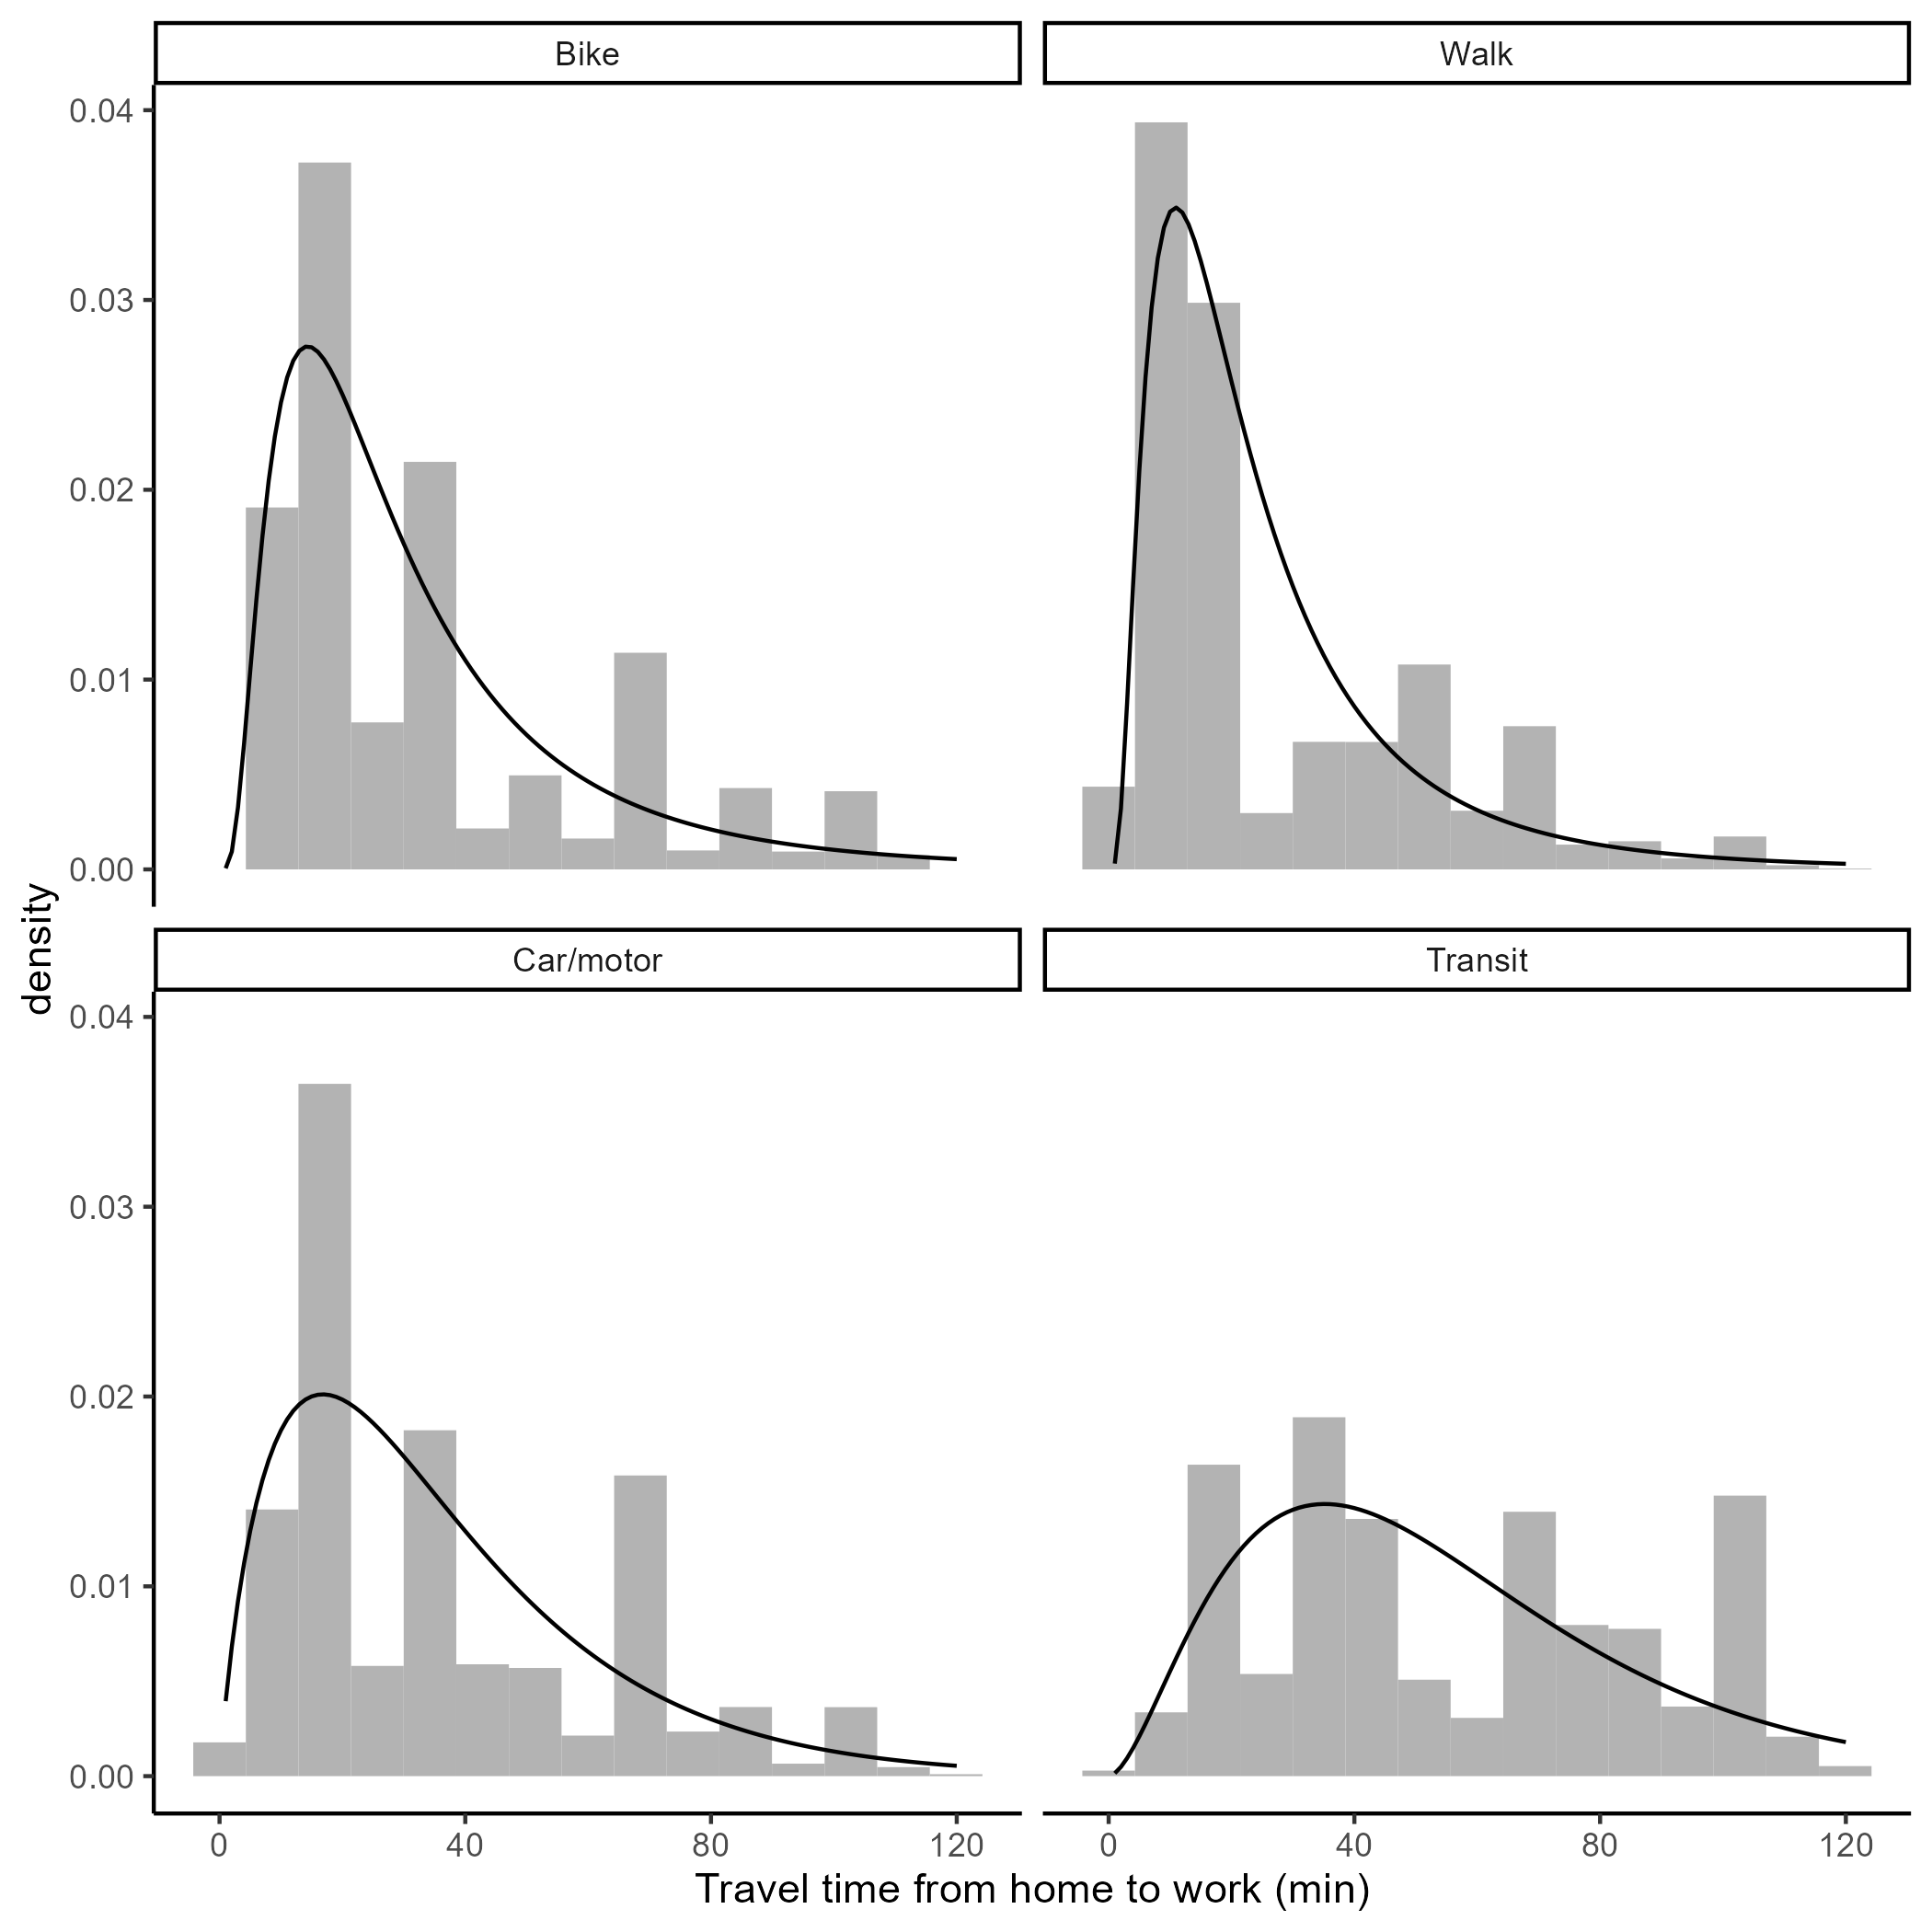
\includegraphics[width=0.85\linewidth]{images/Fig4} 

}

\caption{\label{fig:Fig4} Fitted impedance function against empirical TLD (bars) corresponding to the home to full-time work origin destination flows for the City of Madrid from the 2018 travel survey.}\label{fig:tlds-curves-m-plot}
\end{figure}

\hypertarget{results}{%
\subsection{Results}\label{results}}

\DIFdelbegin \DIFdel{At this point, it is worthwhile reiterating that the empirical example
is a snap-shot of spatial availability
by mode using data from the 2018
travel survey. Our purpose in this empirical example is to investigate
the trends in availability of employment opportunities by mode, and
illustrate how spatial availability can be used in discussions about the
competitive advantage of various modes within Madrid Centro. The spatial
availability of jobs \(V_i^m\) is calculated }\DIFdelend \DIFaddbegin \DIFadd{Figure \ref{fig:Fig5} illustrates the multimodal spatial availability
landscape }\DIFaddend for each of the four modes \(m\) at the level of traffic
analysis zones \(i\)\DIFdelbegin \DIFdel{in Madrid and
displayed in Figure \ref{fig:Fig5}. }%DIFDELCMD < 

%DIFDELCMD < \begin{figure}
%DIFDELCMD < 

%DIFDELCMD < {\centering 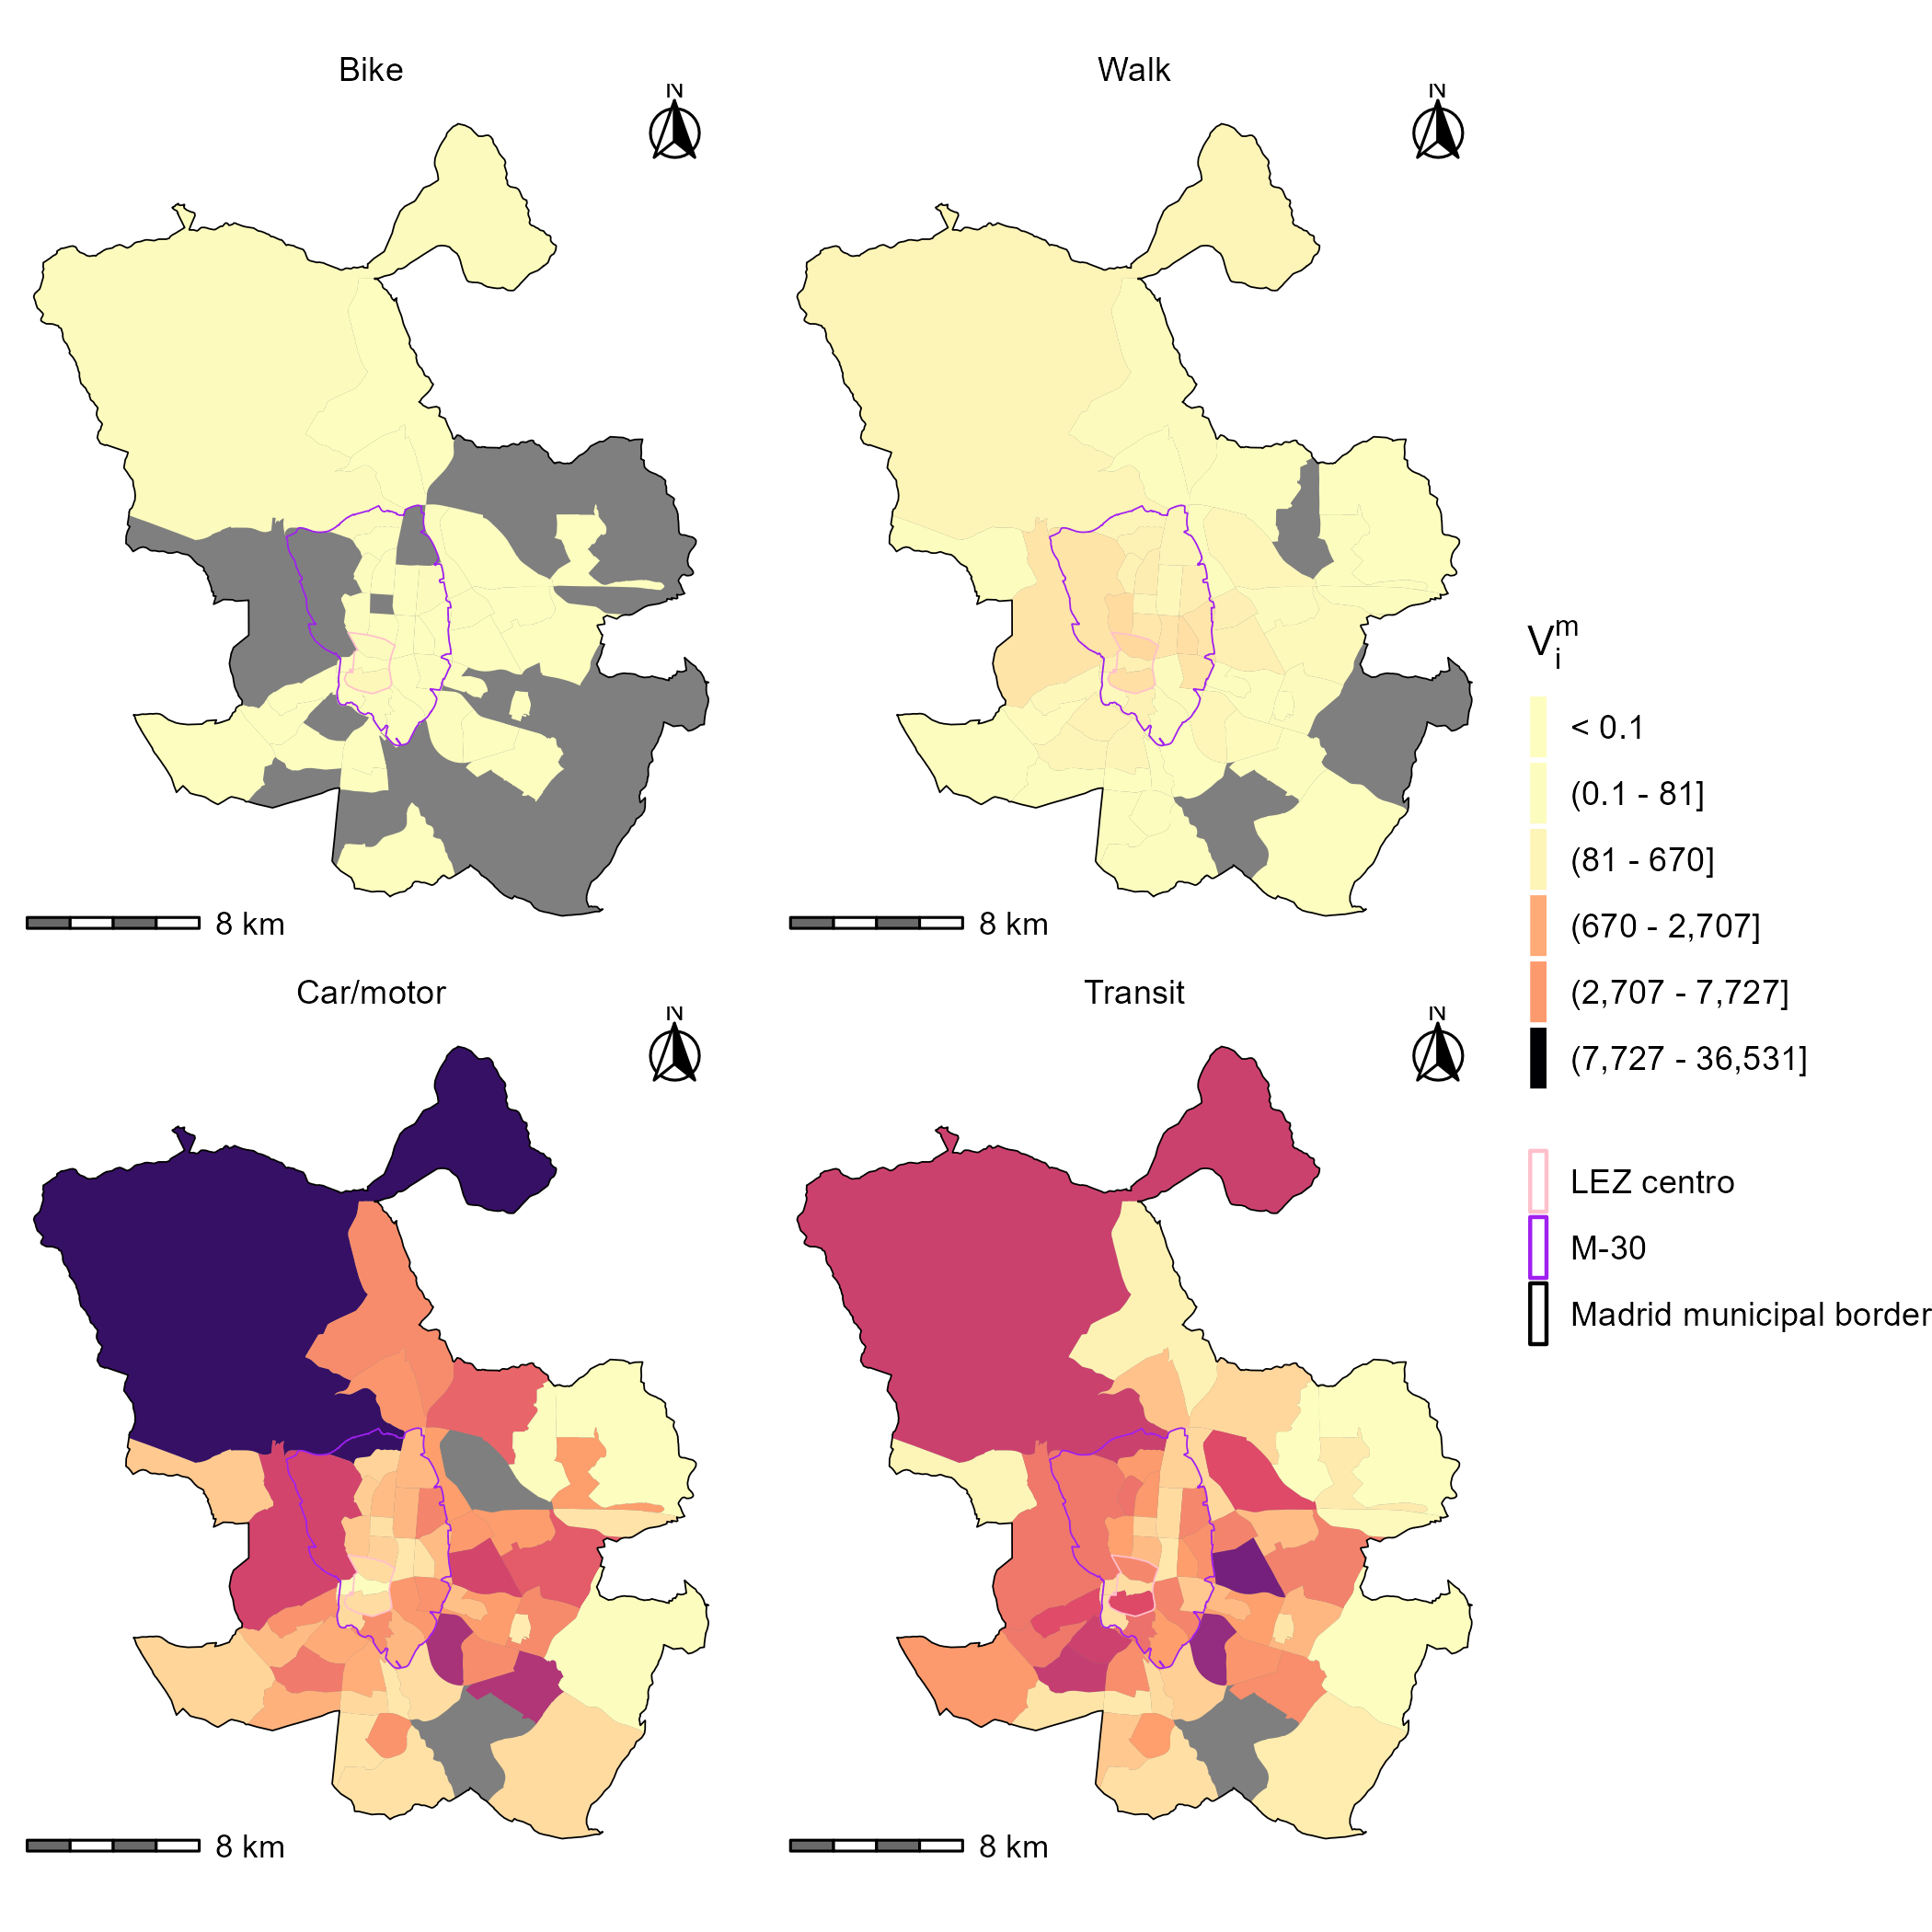
\includegraphics[width=0.85\linewidth]{images/Fig5} 
%DIFDELCMD < 

%DIFDELCMD < }
%DIFDELCMD < 

%DIFDELCMD < %%%
%DIFDELCMD < \caption{%
{%DIFAUXCMD
%DIFDELCMD < \label{fig:Fig5} %%%
\DIFdelFL{Spatial availability of jobs per origin and mode $V_i^m$ in Madrid at the level of TAZ. Grey TAZ have no population. Ranges of values in the legend are quintiles. The TAZ shapefile is available from the Community of Madrid open data portal.}}%DIFAUXCMD
%DIFDELCMD < \label{fig:SA-m-plot}
%DIFDELCMD < \end{figure}
%DIFDELCMD < 

%DIFDELCMD < %%%
\DIFdel{In the figure, }\DIFdelend \DIFaddbegin \DIFadd{. }\DIFaddend \(V_i^m\) is a proportion of the total number of
847,574 jobs in the \DIFdelbegin \DIFdel{region}\DIFdelend \DIFaddbegin \DIFadd{city}\DIFaddend . Since \(V_i^m\) is calculated based on the
population of workers and the distribution of jobs, the values can be
understood as the number of full-time jobs that are spatially available
to full-time workers at that \(i\) traveling by mode \(m\), relative to
all the jobs in the city.
\DIFaddbegin 

\begin{figure}

{\centering 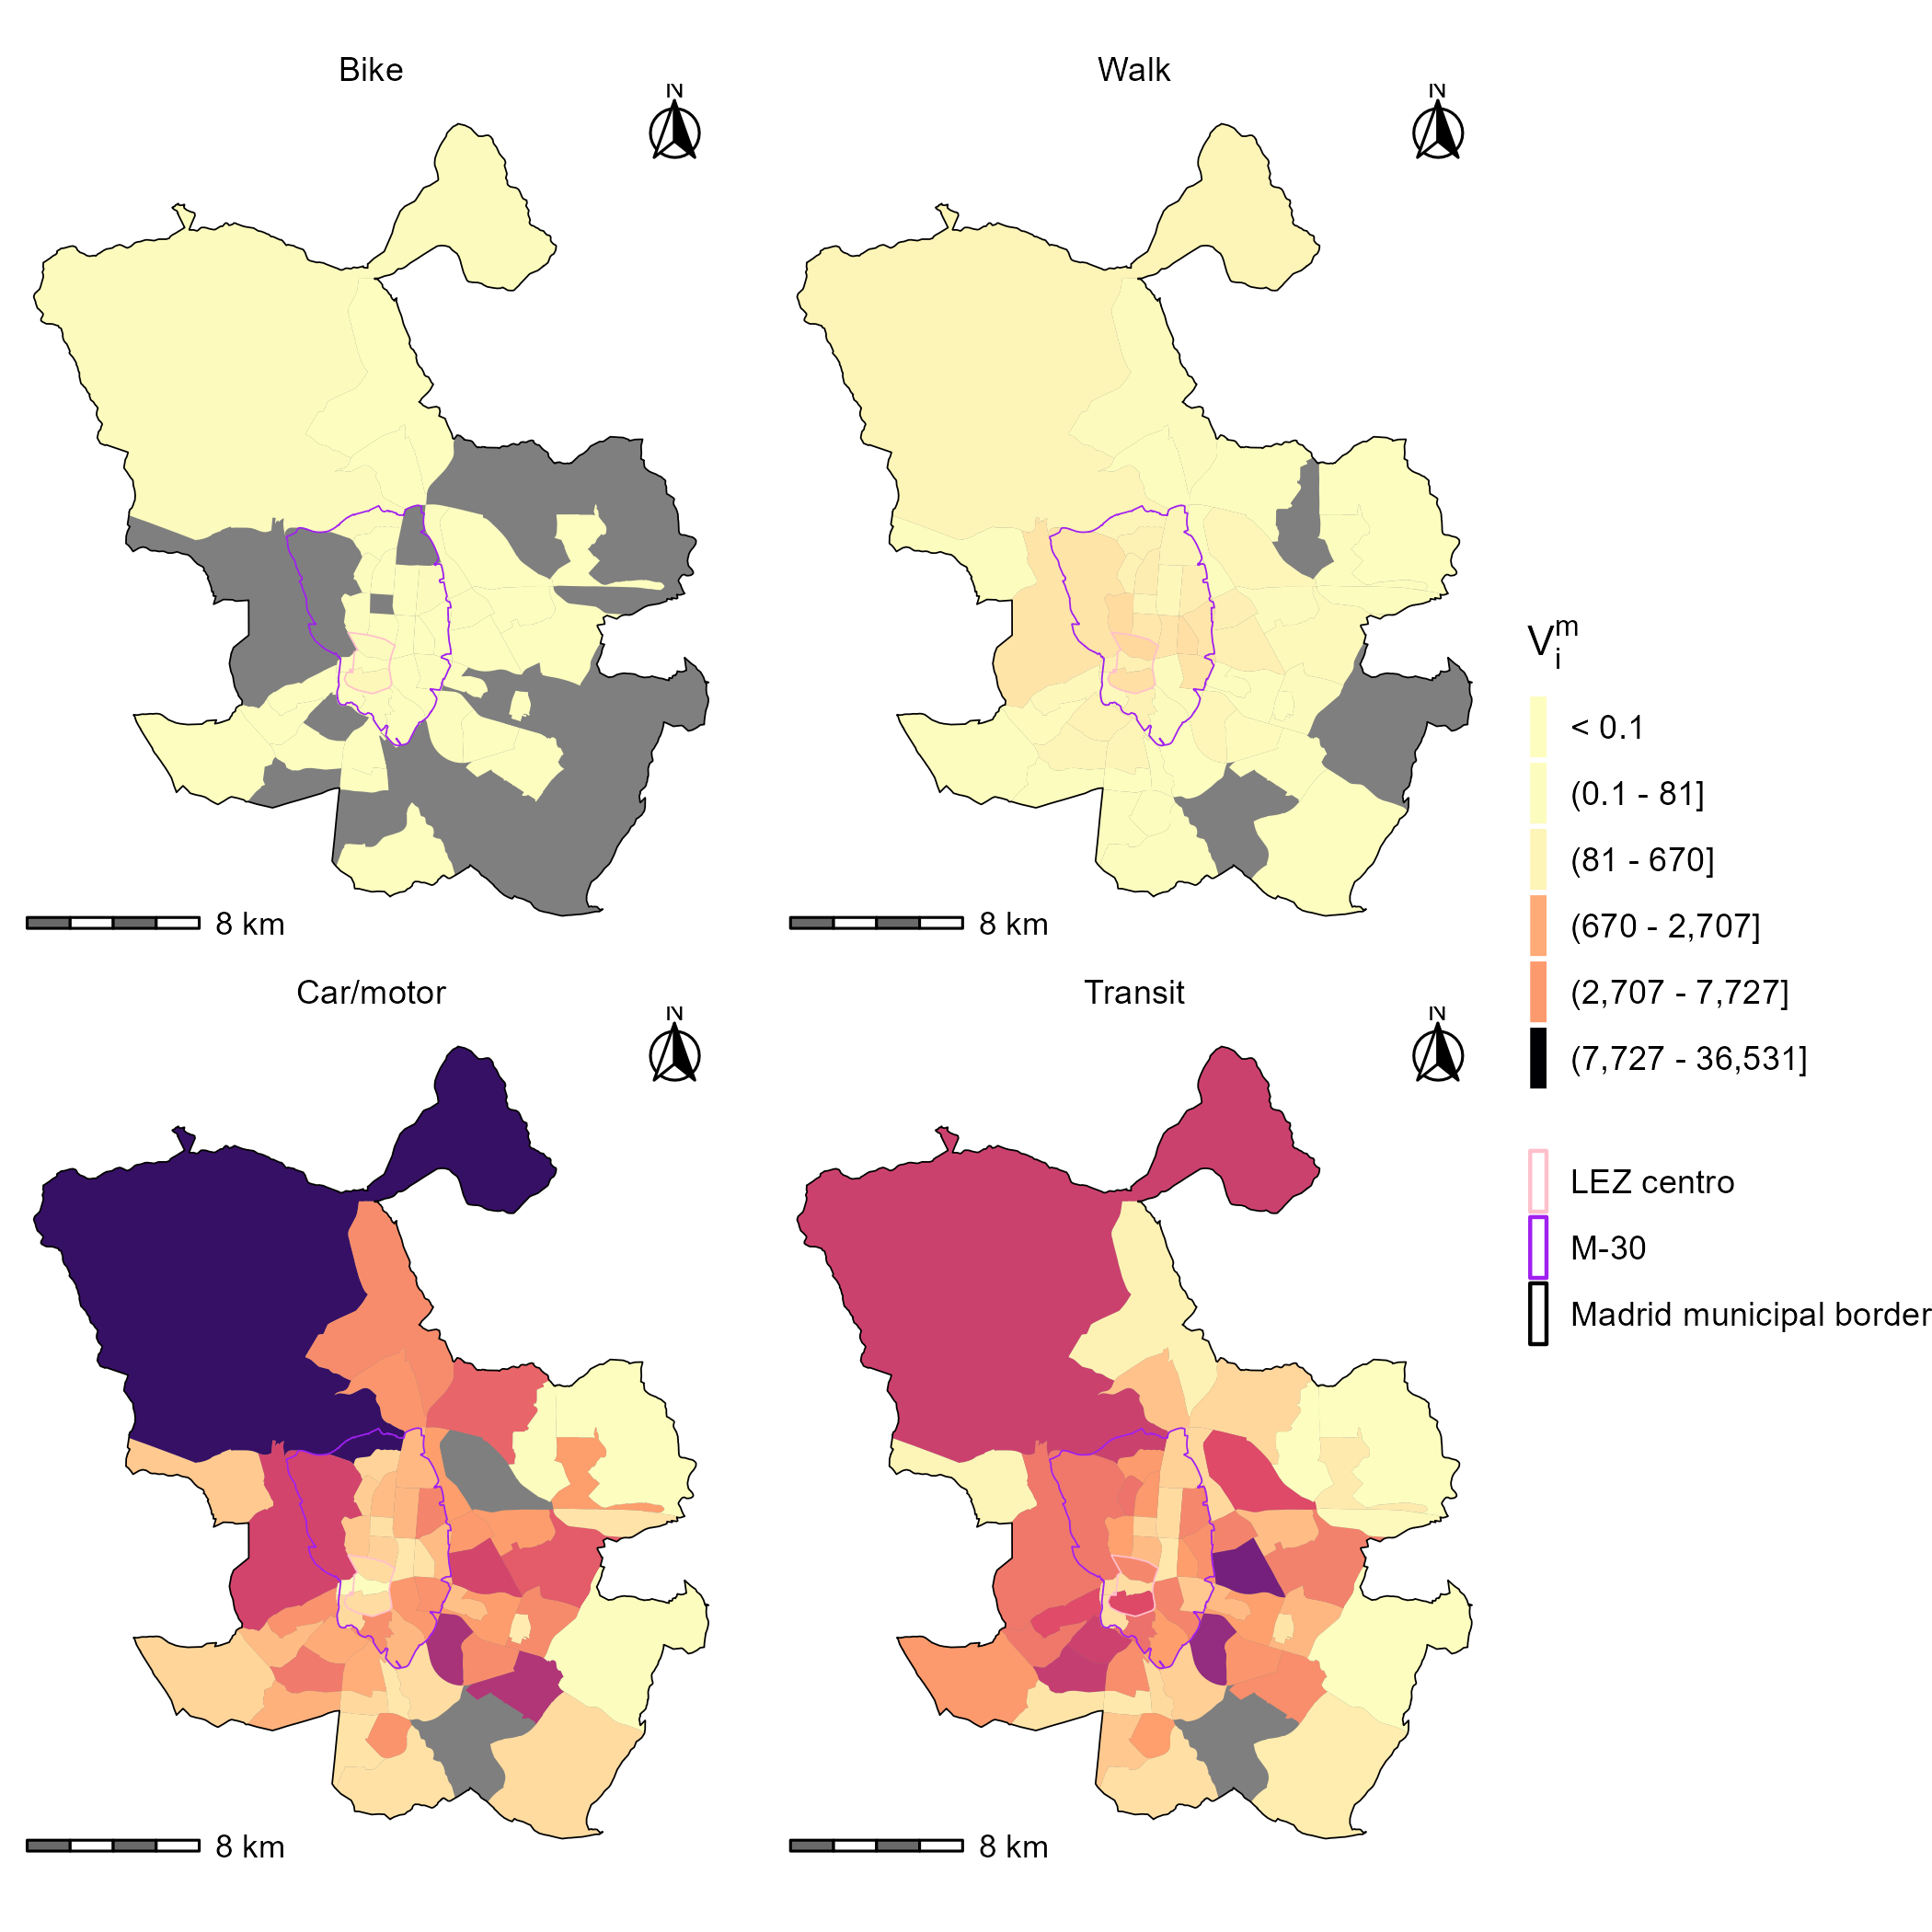
\includegraphics[width=0.85\linewidth]{images/Fig5} 

}

\caption{\label{fig:Fig5} \DIFaddFL{Spatial availability of jobs per origin and mode $V_i^m$ in Madrid at the level of TAZ. Grey TAZ have no population. Ranges of values in the legend are quintiles. The TAZ shapefile is available from the Community of Madrid open data portal.}}\label{fig:SA-m-plot}
\end{figure}

\DIFadd{Figure \ref{fig:Fig5} is a snapshot of the spatial availability as
reflected by the multimodal origin-destination flows and travel times
from the 2018 travel survey: it incorporates the travel behaviour after
LEZ implementation i.e., reduced car trips into the LEZ Centro.
Furthermore, this implementation of spatial availability assumes that
all employment opportunities are of interest to the entire population.
Also, opportunities are proportionally allocated to mode-using
populations based on travel time and mode-using population residing in
the zones relative to the total travel time and population.
}

\DIFaddend There are noticeable differences in the magnitude of \(V_i^m\) between
modes\DIFdelbegin \DIFdel{as seen in Figure \ref{fig:Fig5}.
The }\DIFdelend \DIFaddbegin \DIFadd{. In Figure \ref{fig:Fig5}, the }\DIFaddend majority of \(V_i^m\) \DIFdelbegin \DIFdel{(which is to say of spatially available jobs)
}\DIFdelend are allocated
to workers travelling by car and transit. \DIFdelbegin \DIFdel{In a way, this
is to }\DIFdelend \DIFaddbegin \DIFadd{This can }\DIFaddend be expected since
users of these modes represent 84.1\% of the total population. \DIFdelbegin \DIFdel{However, the }\DIFdelend \DIFaddbegin \DIFadd{The
}\DIFaddend ability to travel at greater speeds also \DIFdelbegin \DIFdel{impacts these results. Furthermore}\DIFdelend \DIFaddbegin \DIFadd{advantages these modes compared
to the non-motorized modes. However}\DIFaddend , differences in \DIFdelbegin \DIFdel{\(V_i^m\) values within modes also }\DIFdelend \DIFaddbegin \DIFadd{\(V_i^\text{car}\)
and \(V_i^\text{transit}\) values }\DIFaddend exist in space: car users outside of
the M-30 \DIFdelbegin \DIFdel{region
appear to enjoy }\DIFdelend \DIFaddbegin \DIFadd{are allocated }\DIFaddend greater spatial availability, while some zones
inside the M-30 \DIFdelbegin \DIFdel{to }\DIFdelend have greater spatial availability for transit. Overall,
the magnitude of \(V_i^m\) values for \DIFdelbegin \DIFdel{cyclists and pedestrians }\DIFdelend \DIFaddbegin \DIFadd{non-motorized mode-users }\DIFaddend are lower
than for car and transit\DIFaddbegin \DIFadd{, }\DIFaddend but the highest values of \(V_i^{bike}\) and
\(V_i^{walk}\) tend to be found in zones within the M-30 and origins
with higher \DIFdelbegin \DIFdel{spatial availability by transit}\DIFdelend \DIFaddbegin \DIFadd{\(V_i^{transit}\)}\DIFaddend .

\DIFdelbegin \DIFdel{The differences between the shares of modes and their shares of spatially available opportunities highlights the competitive advantage
of certain modes, although this effect is not geographically uniform. As
seen in }\DIFdelend \DIFaddbegin \DIFadd{To highlight the spatial differences in modal competitive advantage,
Figure \ref{fig:Fig6} displays the spatial availability and population
per mode aggregated for three areas of }\DIFaddend the \DIFaddbegin \DIFadd{city. Shifting focus to the
}\DIFaddend left-most \DIFdelbegin \DIFdel{columns }\DIFdelend \DIFaddbegin \DIFadd{bars }\DIFaddend of Figure \ref{fig:Fig6}, \DIFdelbegin \DIFdel{users of
`car/motor' and `transit' together }\DIFdelend \DIFaddbegin \DIFadd{motorised mode users }\DIFaddend can avail
95.3\% of all jobs in the city (Spatial Availability by Mode). However,
car \DIFdelbegin \DIFdel{/motor users have }\DIFdelend \DIFaddbegin \DIFadd{users are allocated }\DIFaddend a disproportionate share of \DIFdelbegin \DIFdel{\(V_i^m\) relative to the populationof users
of this mode (Population by Mode), compared to opportunities that are
spatially available to transit users}\DIFdelend \DIFaddbegin \DIFadd{spatial availability
relative to their city-wide population}\DIFaddend . The combined population of car
and transit users is 36.6\% and 47.5\% respectively, \DIFdelbegin \DIFdel{but }\DIFdelend \DIFaddbegin \DIFadd{and }\DIFaddend these
populations are \DIFaddbegin \DIFadd{respectively }\DIFaddend allocated 48.0\% and 47.3\% \DIFdelbegin \DIFdel{respectively, }\DIFdelend of the city's
\DIFdelbegin \DIFdel{jobs. When treating }\DIFdelend \DIFaddbegin \DIFadd{job availability. When conceptualising }\DIFaddend the number of opportunities
\DIFdelbegin \DIFdel{that can be reached }\DIFdelend \DIFaddbegin \DIFadd{accessed }\DIFaddend as a finite value (total: 847,574 \DIFdelbegin \DIFdel{opportunities}\DIFdelend \DIFaddbegin \DIFadd{jobs}\DIFaddend ), fewer opportunities
are spatially available to \DIFdelbegin \DIFdel{slower modes(i.e., walking and cycling), even taking into
account that their share is smaller overall. These modes }\DIFdelend \DIFaddbegin \DIFadd{lesser competitive modes. Modes }\DIFaddend are at a
disadvantage \DIFdelbegin \DIFdel{as a result of: the travel impedance for longer trips }\DIFdelend \DIFaddbegin \DIFadd{when relative travel cost is high }\DIFaddend (see Figure
\ref{fig:Fig4}\DIFdelbegin \DIFdel{; their low population values values overall; and larger populations in origins with high shares of travel
by motorised
modes.
These factors all contribute to the the car/motor mode being most
advantaged in capturing spatially available job opportunities overall.
}\DIFdelend \DIFaddbegin \DIFadd{) and the mode-using population is relatively small
compared to all populations (especially populations with lower travel
costs).
}\DIFaddend 

\begin{figure}

{\centering 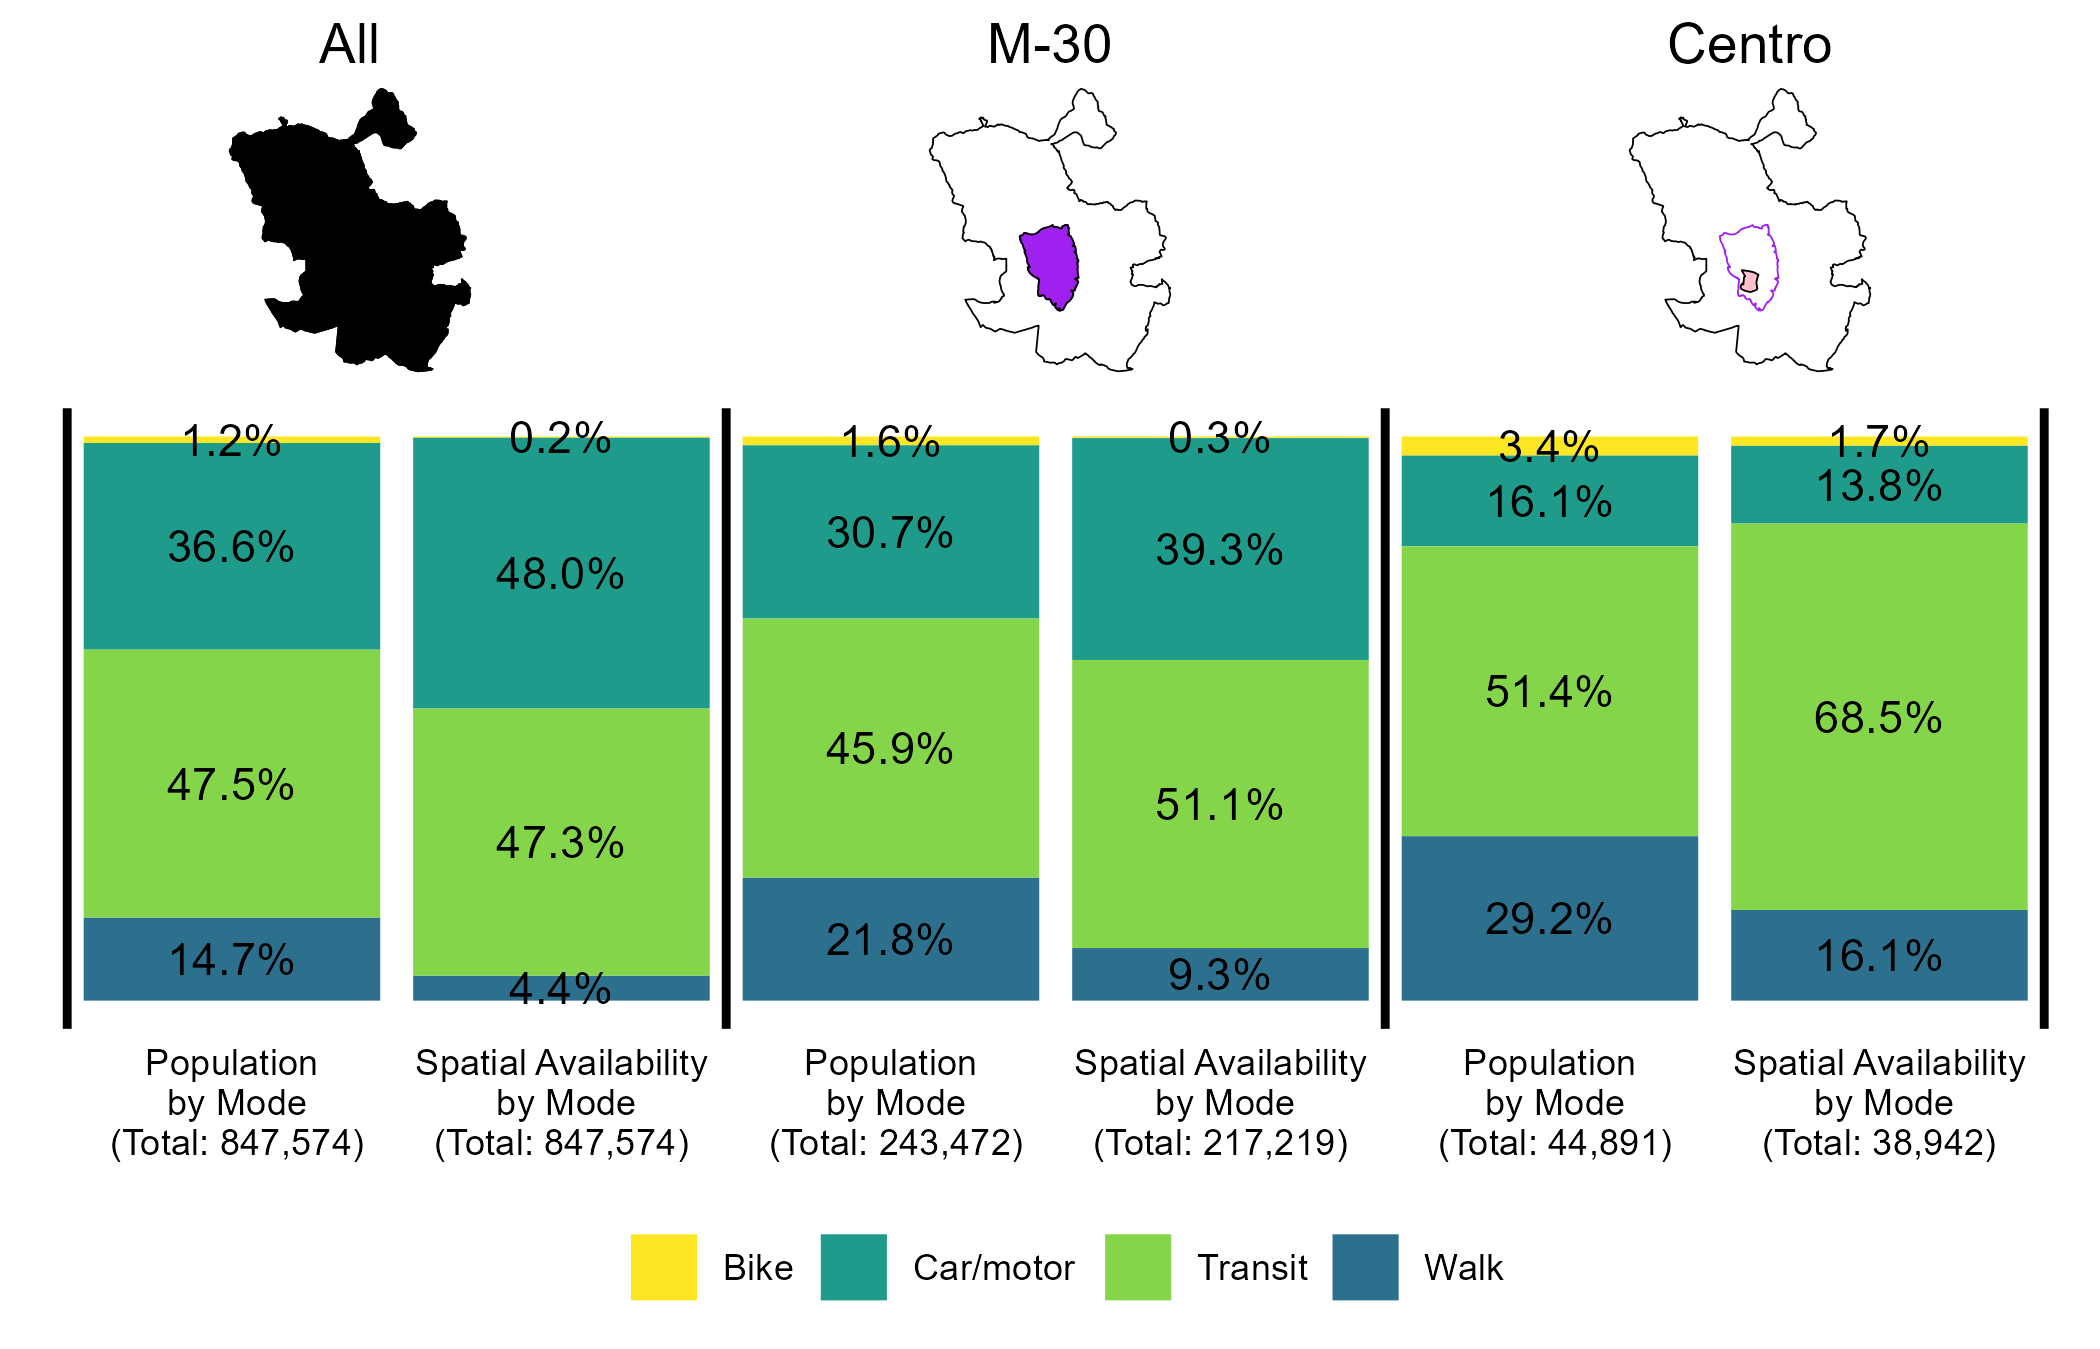
\includegraphics[width=0.85\linewidth]{images/Fig6} 

}

\caption{\label{fig:Fig6} Proportion of population by mode and spatial availability of jobs by mode aggregated for three areas. From left to right, the city of Madrid (All), the area within the M-30 highway (M-30), the area within the Centro region (Centro).}\label{fig:modal-V-comps-plot}
\end{figure}

\DIFdelbegin \DIFdel{The big picture demonstrates how car is the most advantageous mode, however it is interesting to notice that this advantage appears to be
blunted by the LEZ. Unlike the results for the whole city and even
within the M-30 ring, the proportion of car users in Centrois larger
than the proportion of opportunities spatially available to them. The
restriction on cars in effect reduces competition by this mode, and
leads to a relative increment of the mass effect of the modes allowed
within the LEZ, which also contains a large number of jobs (see Figure
\ref{fig:Fig2}). }\DIFdelend \DIFaddbegin \DIFadd{Though car mode offers the most spatial availability overall, this is
not the case within the Centro. }\DIFaddend As summarized in the two right-most \DIFdelbegin \DIFdel{columns }\DIFdelend \DIFaddbegin \DIFadd{bars
}\DIFaddend in Figure \ref{fig:Fig6}, the proportion of jobs spatially available to
car \DIFaddbegin \DIFadd{users }\DIFaddend in Centro is \DIFdelbegin \DIFdel{(}\DIFdelend 13.8\% \DIFdelbegin \DIFdel{or }\DIFdelend \DIFaddbegin \DIFadd{(}\DIFaddend 5,373 opportunities)\DIFdelbegin \DIFdel{. For reference, this is }\DIFdelend \DIFaddbegin \DIFadd{, }\DIFaddend less than the
proportion of the car users in \DIFaddbegin \DIFadd{the }\DIFaddend Centro (16.1\%)\DIFdelbegin \DIFdel{, evidently less
then the proportion of car users in the
city, and is the opposite of the
overall trend }\DIFdelend \DIFaddbegin \DIFadd{. The trend in the
Centro for car-users is opposite to that of the city overall }\DIFaddend (left-most
\DIFdelbegin \DIFdel{columns) and within the }\DIFdelend \DIFaddbegin \DIFadd{bars) and the areas inside the }\DIFaddend M-30 (middle \DIFdelbegin \DIFdel{columns). }%DIFDELCMD < 

%DIFDELCMD < %%%
\DIFdel{It is also clear that
more opportunities are spatially available to
}\DIFdelend \DIFaddbegin \DIFadd{bars). We suspect that
car-mode's competitive advantage is blunted by the LEZ: the number of
car trips are relatively reduced in the area making }\DIFaddend non-car \DIFdelbegin \DIFdel{users within Centro. In the case of active travel, the proportions of cyclists and walkers within LEZ Centro still exceeds the proportions of jobs
spatially available to them --- however, the disparity is drastically reduced compared to the rest of the city. As
seen in Figure \ref{fig:Fig6}, there is a higher proportion of
opportunities that are
spatially available to pedestrians and cyclists
in Centro than in the City overall and in areas within the M-30.
Notably, within Centro, }\DIFdelend \DIFaddbegin \DIFadd{modes more
competitive. Car mode's advantage in the Centro is also diminished by
the relative increment of the mass effect and concentration of jobs
(Figure \ref{fig:Fig2}) within/around the Centro.
}

\DIFadd{Since car mode is less competitive within the Centro, other modes are
relatively }\emph{\DIFadd{more}} \DIFadd{competitive. Referring to the active travel modes
in the right-most bars in Figure \ref{fig:Fig6}, }\DIFaddend 1.7\% and 16.1\% of
opportunities are spatially available to bike and walk modes
respectively, while their populations represent 1.2\% and 14.7\% of the
population. \DIFdelbegin \DIFdel{By }\DIFdelend \DIFaddbegin \DIFadd{The disparity between the proportions of cyclists and
walkers and the proportions of jobs spatially available to them is
}\emph{\DIFadd{smaller}} \DIFadd{than displayed in the other two aggregations (All and
M-30). We suspect that by }\DIFaddend restricting the ability of cars to enter
Centro, the LEZ \DIFdelbegin \DIFdel{seems to contribute to }\DIFdelend \DIFaddbegin \DIFadd{contributes to }\DIFaddend leveling the playing field for slower
modes, in particular cycling and walking \DIFdelbegin \DIFdel{, }\DIFdelend but also transit. \DIFdelbegin \DIFdel{As seen in the Figure \ref{fig:Fig6}, transit }\DIFdelend \DIFaddbegin \DIFadd{Transit }\DIFaddend users
are generally close to parity \DIFdelbegin \DIFdel{across the region}\DIFdelend \DIFaddbegin \DIFadd{city-wide (left-most bars)}\DIFaddend , with nearly as
many spatially available jobs as transit users. Still, \DIFdelbegin \DIFdel{this }\DIFdelend \DIFaddbegin \DIFadd{transit }\DIFaddend mode has
the greatest advantage in \DIFdelbegin \DIFdel{LEZ }\DIFdelend \DIFaddbegin \DIFadd{the }\DIFaddend Centro with 68.5\% of spatially available
jobs \DIFdelbegin \DIFdel{in Centro }\DIFdelend for 51.4\% of transit users in Centro. This result makes intuitive
sense: after car, \DIFdelbegin \DIFdel{it }\DIFdelend \DIFaddbegin \DIFadd{transit }\DIFaddend is the mode with the greatest range \DIFdelbegin \DIFdel{, andunlike car it is unrestricted in the LEZCentro}\DIFdelend \DIFaddbegin \DIFadd{and,
unlike car, it faced no restrictions by the LEZ}\DIFaddend .

The spatial differences in the competitive \DIFdelbegin \DIFdel{dis/}\DIFdelend \DIFaddbegin \DIFadd{(dis)}\DIFaddend advantage of spatial
availability between modes can also be visualized at a finer level of
\DIFaddbegin \DIFadd{spatial }\DIFaddend granularity. Figure \ref{fig:Fig7} shows \(v_i^m\), the spatial
availability \(V_i^m\) divided by the population of users of \(m\).
Values of \(v_i^m\) below one are shown in shades of orange, and
indicate TAZs with less than one spatially available opportunity per
capita for the mode. Values above one are shown in shades of green, and
indicate TAZs with more than one spatially available opportunity per
capita for the mode. The highest spatial availability per capita (shown
in blue) is for car users in a zone northeast just beyond the M-30.
These plots illustrate in unambiguous fashion, and in a quantity that is
comparable over space and time, the advantage in terms of spatial
availability of car for most of the city (bottom left plot, areas
denoted with green \(v_i^m\) values above one). It can also be observed
that spatial availability of jobs is relatively well balanced for
transit users over most of the regions (i.e., many zones are light
\DIFdelbegin \DIFdel{orange or light }\DIFdelend green). \DIFdelbegin \DIFdel{Spatial }\DIFdelend \DIFaddbegin \DIFadd{In contrast, spatial }\DIFaddend availability of jobs for non-motorised
modes \DIFdelbegin \DIFdel{, in contrast, }\DIFdelend is low (under one) overall, although less so within\DIFaddbegin \DIFadd{/around the }\DIFaddend LEZ
Centro.

\begin{figure}

{\centering 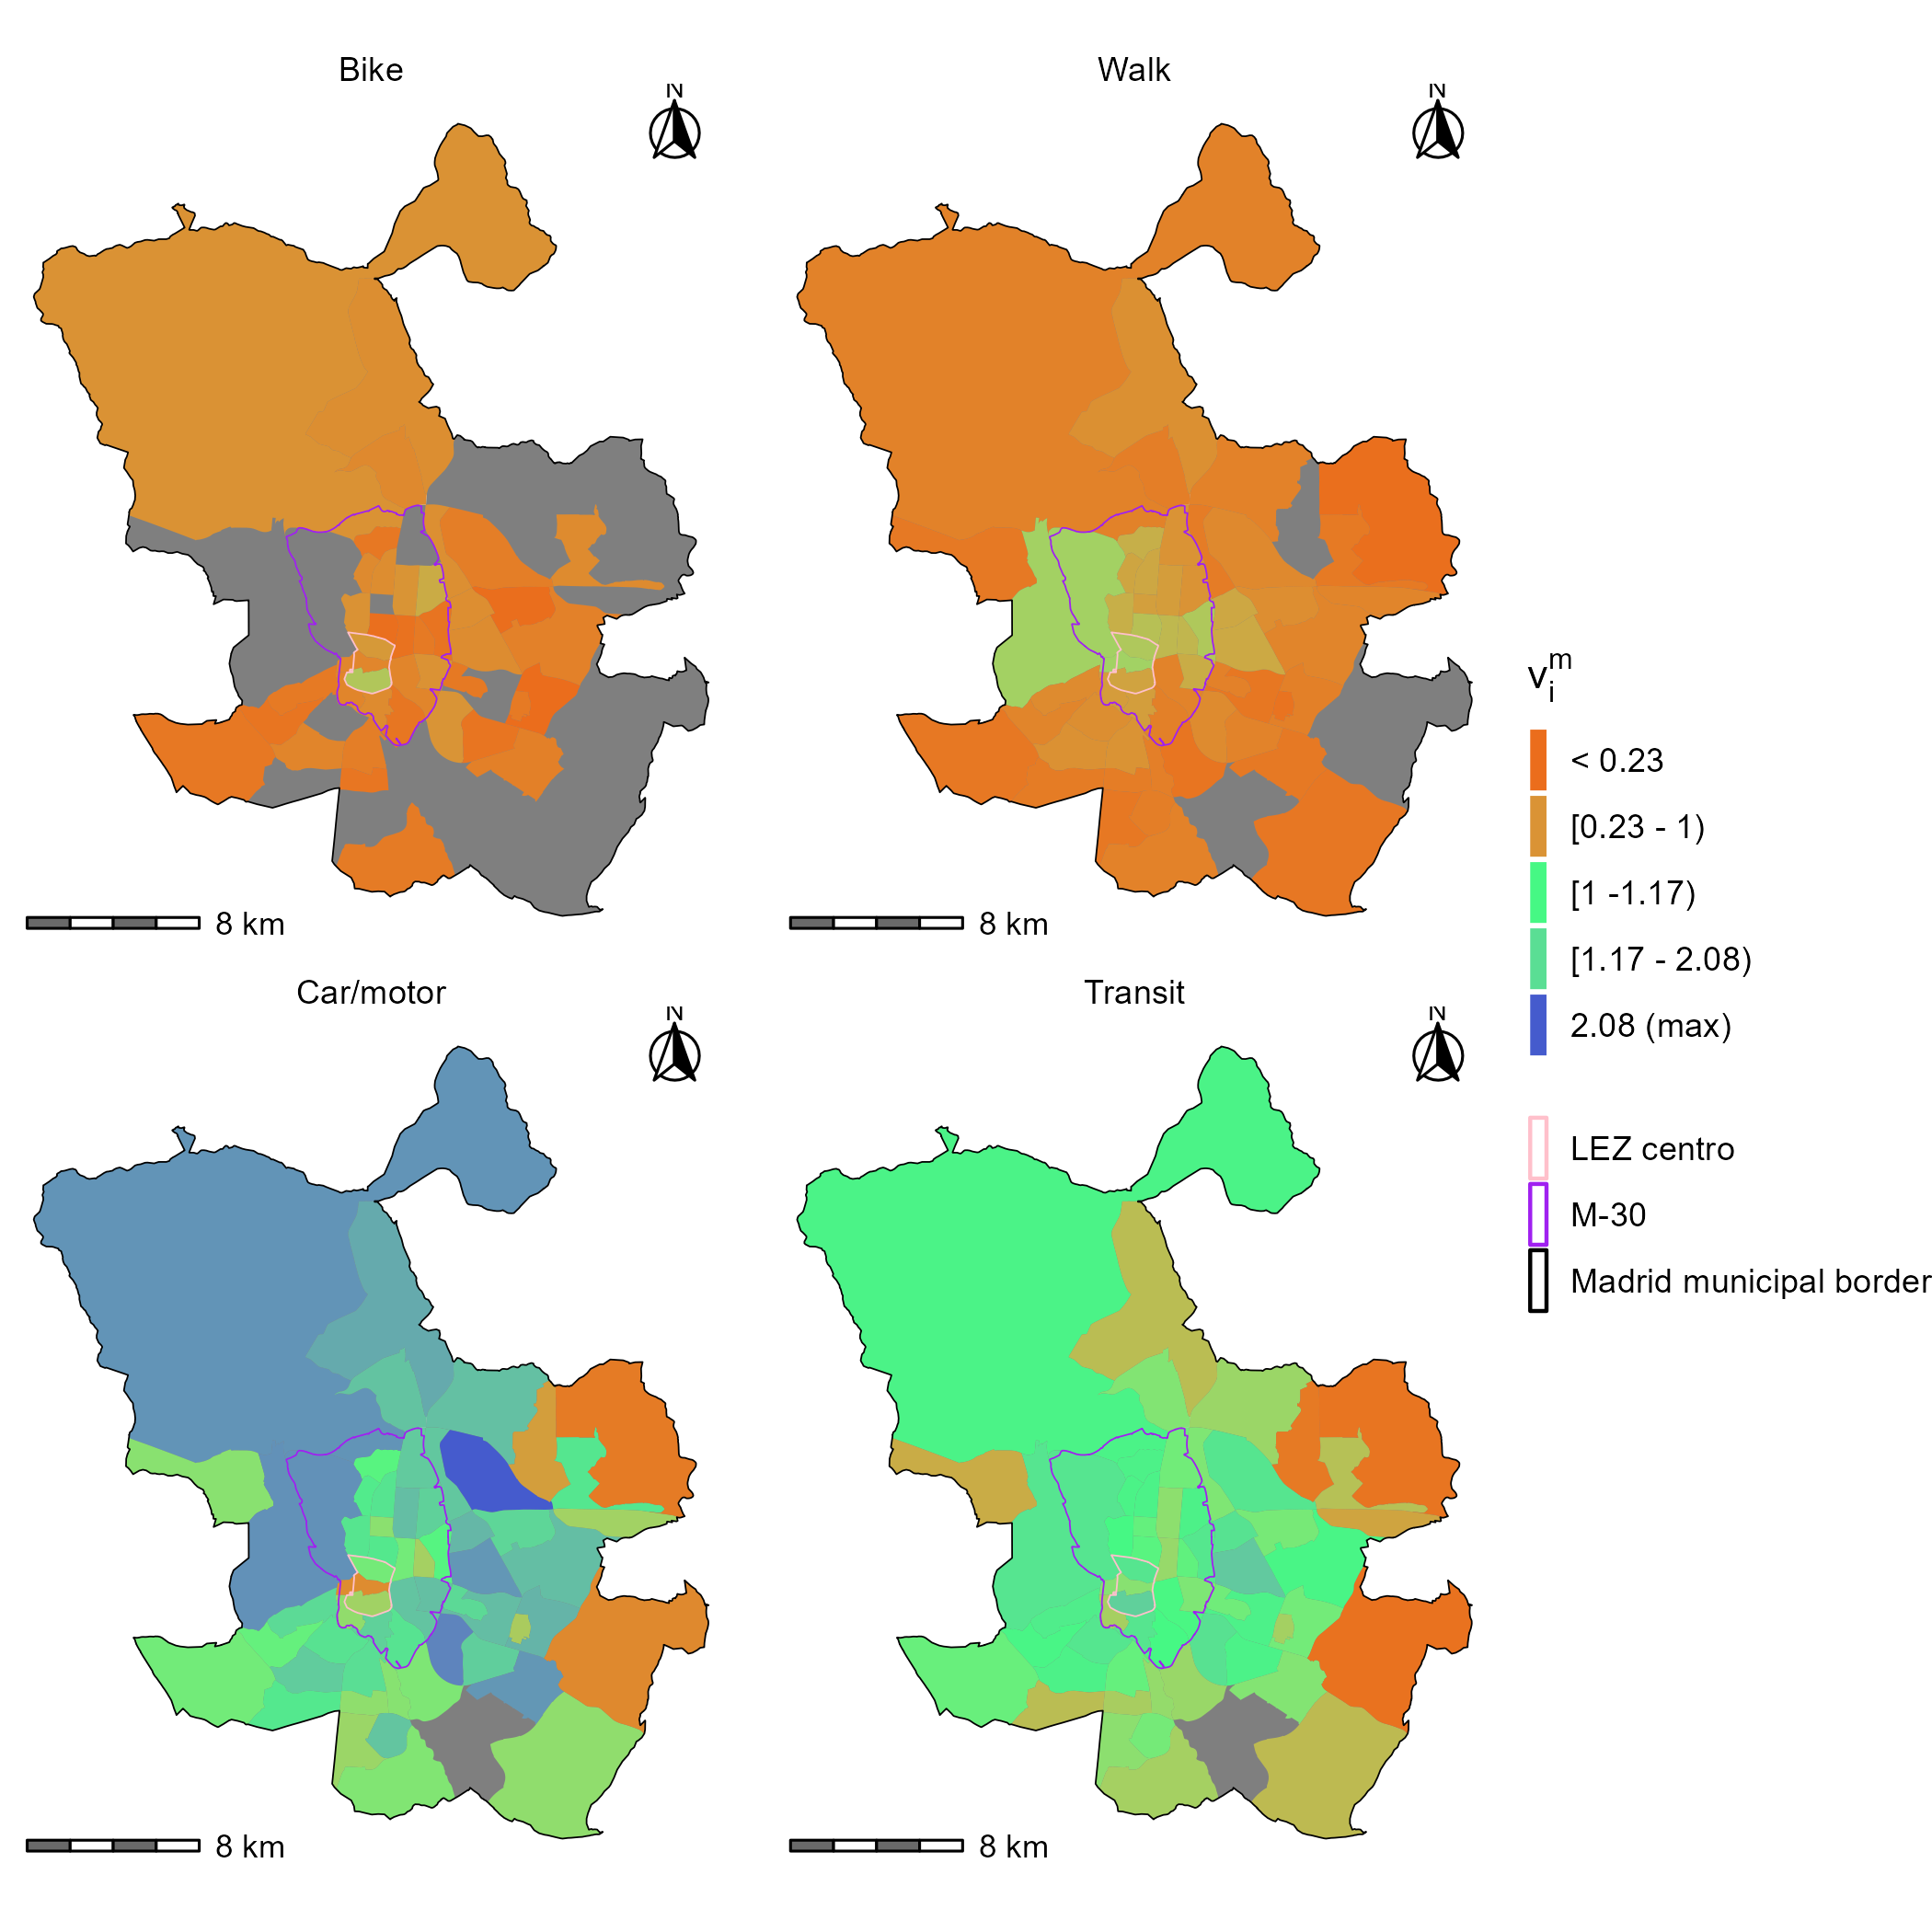
\includegraphics[width=0.85\linewidth]{images/Fig7} 

}

\caption{\label{fig:Fig7} Distribution of spatially available jobs per capita by mode of transportatin ($v_i^m$) represented at the level of TAZ. Grey TAZ have no population that use the mode. Ranges of values in the legend are quintiles. The TAZ shapefile is available from the Community of Madrid open data portal.}\label{fig:SA-per-capita-m-plot}
\end{figure}

\DIFdelbegin \DIFdel{Incidentally, }\DIFdelend \DIFaddbegin \DIFadd{Since }\DIFaddend \(v_i^m\) values \DIFdelbegin \DIFdel{for car within and near LEZ Centro is
close to or below one in Figure \ref{fig:Fig7}, while all non-car modes
have relatively higher \(v_i^m\) values. Since these values }\DIFdelend are comparable across regions and over time,
Figure \ref{fig:Fig7} potentially provides a benchmark for quantifying
changes in LEZ policies in the future. \DIFdelbegin \DIFdel{As Figure \ref{fig:Fig7} also shows, many areas }\DIFdelend \DIFaddbegin \DIFadd{Even }\DIFaddend within the M-30\DIFdelbegin \DIFdel{have high (white/green) \(v_i^m\) values for car, but the
results for LEZ Centro }\DIFdelend \DIFaddbegin \DIFadd{, \(v_i^car\)
values are still high (over 1) for most zones. These results may }\DIFaddend give
reasonable grounds to speculate that a spatial expansion of the LEZ to
include all areas within the M-30 would \DIFdelbegin \DIFdel{likely }\DIFdelend increase the spatial
availability of jobs for transit users, cyclists and pedestrians.
\DIFaddbegin \DIFadd{However, further investigation is needed.
}\DIFaddend 

\hypertarget{discussion-and-conclusions}{%
\section{Discussion and conclusions}\label{discussion-and-conclusions}}

Accessibility measures are an important tool in transportation research
{[}9{]} and are increasingly seen as valuable for planning purposes
{[}4--8{]}. They boast a long history of development, beginning with
Hansen-type \(S_i^m\) measures, with other developments like Shen's
\(a_i^m\), to account for competition/congestion. The more recent
spatial availability measure \(V_i^m\) has in common with these
accessibility indicators that it is a weighted sum of the opportunities
in a region from the perspective of a determined origin \(i\).
Aggregations of opportunities embody principles of gravitational/spatial
interaction modelling that date back to at least H.C. Carey {[}\DIFdelbegin \DIFdel{50}\DIFdelend \DIFaddbegin \DIFadd{62}\DIFaddend {]},
and are part of a line of research that includes the work of Ravenstein
{[}\DIFdelbegin \DIFdel{51}\DIFdelend \DIFaddbegin \DIFadd{63}\DIFaddend {]}, Reilly {[}\DIFdelbegin \DIFdel{52}\DIFdelend \DIFaddbegin \DIFadd{64}\DIFaddend {]}, Stewart {[}\DIFdelbegin \DIFdel{53--55}\DIFdelend \DIFaddbegin \DIFadd{65--67}\DIFaddend {]}, Zipf {[}\DIFdelbegin \DIFdel{56,57}\DIFdelend \DIFaddbegin \DIFadd{68,69}\DIFaddend {]},
Wilson {[}\DIFdelbegin \DIFdel{37}\DIFdelend \DIFaddbegin \DIFadd{49}\DIFaddend {]}, and many others. In this way, \(S_i^m\), \(a_i^m\), and
\DIFdelbegin \DIFdel{yes, }\DIFdelend \(V_i^m\) \DIFdelbegin \DIFdel{, }\DIFdelend can be interpreted as scores of the potential for interaction
with opportunities in space.

Different accessibility indicators are characterized by how they weight
and aggregate opportunities. Spatial availability's contribution to the
literature is to incorporate a proportional allocation mechanism that
essentially constrains the sums to match the number of opportunities in
the region\DIFdelbegin \DIFdel{; in this way }\DIFdelend \DIFaddbegin \DIFadd{: }\DIFaddend it is a singly-constrained accessibility measure that
\DIFdelbegin \DIFdel{naturally }\DIFdelend \DIFaddbegin \DIFadd{natively }\DIFaddend accommodates congestion and competition. The effort with
spatial availability is in line with previous research on proportional
allocation by \DIFdelbegin \DIFdel{Paez }\DIFdelend \DIFaddbegin \DIFadd{Páez }\DIFaddend et al.\DIFaddbegin \DIFadd{~(2019) }\DIFaddend {[}\DIFdelbegin \DIFdel{14}\DIFdelend \DIFaddbegin \DIFadd{12}\DIFaddend {]}. As initially introduced by
Soukhov et al.\DIFaddbegin \DIFadd{~(2023) }\DIFaddend {[}15{]}, spatial availability was designed for a
homogeneous population traveling by a single mode of transportation. In
this paper, we extended spatial availability for the case of
heterogeneous populations. We discussed this in terms of multiple modes
of transportation, but the framework can accommodate equally well
variations in travel behavior by population segments.

An empirical example using data from Madrid \DIFdelbegin \DIFdel{helped }\DIFdelend \DIFaddbegin \DIFadd{helps }\DIFaddend to illustrate the
potential of multimodal spatial availability analysis, including its
ability to account for competition for opportunities within and between
modes. Particularly relevant is the fact that spatial availability
scores relate directly to the total number of opportunities in the
region. This makes it possible to compare the results to intuitive
benchmarks, such as opportunities per population, in ways that other
accessibility measures cannot or tend to obfuscate. This comparability
is preserved between regions and over time. The example suggests that
once \DIFdelbegin \DIFdel{that }\DIFdelend opportunities are treated as \DIFdelbegin \DIFdel{being finite, }\DIFdelend \DIFaddbegin \DIFadd{finite, it could be suggested that
}\DIFaddend restrictions to travel by car \DIFaddbegin \DIFadd{(due to the LEZ) }\DIFaddend leave more spatially
available opportunities for \DIFdelbegin \DIFdel{non-car-users}\DIFdelend \DIFaddbegin \DIFadd{non-car users}\DIFaddend . This difference for car
travel in locations within\DIFdelbegin \DIFdel{and
immediately }\DIFdelend \DIFaddbegin \DIFadd{/}\DIFaddend around the LEZ Centro \DIFdelbegin \DIFdel{seems }\DIFdelend \DIFaddbegin \DIFadd{seem }\DIFaddend to increase the
number of opportunities spatially available to transit users (transit
being the second most competitive mode) \DIFdelbegin \DIFdel{, }\DIFdelend as well as \DIFdelbegin \DIFdel{the spatial availability from
the perspective of }\DIFdelend non-motorised modes.
In effect, a policy such as \DIFdelbegin \DIFdel{Low
Emission Zones help to improve the accessibility }\DIFdelend \DIFaddbegin \DIFadd{LEZ appears to help improve the spatial
availability }\DIFaddend situation of active travel and transit \DIFaddbegin \DIFadd{mode users }\DIFaddend in the
parts of the city where it is implemented\DIFdelbegin \DIFdel{.
}%DIFDELCMD < 

%DIFDELCMD < %%%
\DIFdelend \DIFaddbegin \DIFadd{, though additional research is
needed. To further speculate, the spatial availability allocated to
car-users near but outside the LEZ Centro is still relatively high,
potentially supporting the case for LEZ expansion from this perspective.
}\DIFaddend The purpose of the empirical example is to illustrate the kind of
insights that can be derived from the application of multimodal spatial
availability.
\DIFdelbegin \DIFdel{But there }\DIFdelend \DIFaddbegin 

\DIFadd{There }\DIFaddend are some intriguing opportunities for future research.
Accessibility indicators are not designed to work as modal split models,
and yet, in the case of policies that alter the relative cost of various
forms of transportation, one can reasonably expect to see some shifts
between modes. In our empirical example\DIFaddbegin \DIFadd{, }\DIFaddend we used data collected \DIFdelbegin \emph{\DIFdel{after}} %DIFAUXCMD
\DIFdelend \DIFaddbegin \DIFadd{after
}\DIFaddend the introduction of LEZ Centro. However, given a modal split model to
\DIFdelbegin \DIFdel{project }\DIFdelend \DIFaddbegin \DIFadd{predict }\DIFaddend model shares, accessibility indicators, including spatial
availability, can be used to investigate changes to the accessibility
landscape. \DIFdelbegin \DIFdel{Ditto }\DIFdelend \DIFaddbegin \DIFadd{A similar logic can be applied }\DIFaddend for destination choice. Our
empirical example presented \DIFdelbegin \DIFdel{but }\DIFdelend a snapshot of this, and in future research
it \DIFdelbegin \DIFdel{will
}\DIFdelend \DIFaddbegin \DIFadd{may }\DIFaddend be interesting to investigate changes \DIFaddbegin \DIFadd{in spatial availability
}\DIFaddend \emph{between} policy interventions. The \DIFdelbegin \DIFdel{expansion of }\DIFdelend \DIFaddbegin \DIFadd{plan to expand }\DIFaddend Madrid's LEZ to
the ring contained by the M-30 \DIFdelbegin \DIFdel{orbital }\DIFdelend presents an excellent opportunity\DIFdelbegin \DIFdel{to do so}\DIFdelend . Given
the intuitive \DIFdelbegin \DIFdel{and straightforward }\DIFdelend interpretation of spatial availability scores as fractions
of opportunities from the total, relative and absolute changes in the
\DIFdelbegin \DIFdel{accessibility }\DIFdelend \DIFaddbegin \DIFadd{spatial availability }\DIFaddend landscape can be assessed, thus helping to evaluate
the implications of policy interventions.

\DIFdelbegin \DIFdel{Finally, our }\DIFdelend \DIFaddbegin \DIFadd{Our empirical }\DIFaddend example dealt with differences in travel by mode only, but
it is possible to think of the intersection between mode of travel and
different types of travelers. This would expand the number of
sub-populations in the analysis from, say, \(m=M\) (modes) to
\(m = M\cdot Q\) (modes times population segments), each with their own
characteristic impedance function. Evaluations of this kind will be
especially relevant as LEZ are implemented in cities globally, and the
question of their impact on disadvantaged populations who have become
mobility-restricted increasingly come to the fore {[}\DIFdelbegin \DIFdel{40,58,59}\DIFdelend \DIFaddbegin \DIFadd{52,70,71}\DIFaddend {]}.

\DIFaddbegin \DIFadd{To close, in this work spatial availability considers competition by
allocating opportunities (the subject of the single-constraint) to modal
populations in zones based on zonal proportions. Opportunity congestion
can be seen on a continuum, but how it is to be considered within
accessibility research is an ongoing subject of exploration
}{[}\DIFadd{14,17,18}{]}\DIFadd{. It is in this context we present spatial availability
and its multimodal extension. While our focus was on a multiple modes,
this consideration is just one case of heterogeneous populations (i.e.,
travel by different modes). The multimodal method itself can easily
accommodate other forms of population or opportunity heterogeneity, for
example: variations in rich and poor, young and old, types of
opportunities. Like preceding accessibility measures, the potential
applications of spatial availability are as numerous as the potential
study contexts.
}

\DIFaddend \hypertarget{author-contributions}{%
\section{Author contributions}\label{author-contributions}}

The authors confirm contribution to the paper as follows: study
conception and design: AS, JTO, JSL, AP.; data collection: AS, JTO,
JSL.; analysis and interpretation of results: AS, JTO, JSL, AP.; draft
manuscript preparation: AS, JSL, AP. All authors reviewed the results
and approved the final version of the manuscript.

\hypertarget{references}{%
\section*{References}\label{references}}
\addcontentsline{toc}{section}{References}

\hypertarget{refs}{}
\begin{CSLReferences}{0}{0}
\leavevmode\vadjust pre{\hypertarget{ref-hansenHowAccessibilityShapes1959}{}}%
\CSLLeftMargin{1. }%
\CSLRightInline{Hansen WG. How accessibility shapes land use. Journal of
the American Institute of Planners. 1959;25: 73--76.
doi:\href{https://doi.org/10.1080/01944365908978307}{10.1080/01944365908978307}}

\leavevmode\vadjust pre{\hypertarget{ref-geursAccessibility2004}{}}%
\CSLLeftMargin{2. }%
\CSLRightInline{Geurs KT, Wee B van. Accessibility evaluation of
land-use and transport strategies: Review and research directions.
Journal of Transport Geography. 2004;12: 127--140. Available:
\href{http://www.sciencedirect.com/science/article/B6VG8-4B28VY7-1/2/61478339c14cab4fa58438ad7b1f4610\%0AC:/Papers/Journal\%20of\%20Transport\%20Geography/Journal\%20of\%20Transport\%20Geography\%20(2004)\%2012\%20(2)\%20127-140.pdf}{http://www.sciencedirect.com/science/article/B6VG8-4B28VY7-1/2/61478339c14cab4fa58438ad7b1f4610
C:/Papers/Journal of Transport Geography/Journal of Transport Geography
(2004) 12 (2) 127-140.pdf}}

\leavevmode\vadjust pre{\hypertarget{ref-paezPositive2012}{}}%
\CSLLeftMargin{3. }%
\DIFdelbegin %DIFDELCMD < \CSLRightInline{Paez A, Scott DM, Morency C. Measuring accessibility:
%DIFDELCMD < Positive and normative implementations of various accessibility
%DIFDELCMD < indicators. Journal of Transport Geography. 2012;25: 141--153.
%DIFDELCMD < doi:\href{https://doi.org/10.1016/j.jtrangeo.2012.03.016}{10.1016/j.jtrangeo.2012.03.016}}
%DIFDELCMD < %%%
\DIFdelend \DIFaddbegin \CSLRightInline{Páez A, Scott DM, Morency C. Measuring accessibility:
Positive and normative implementations of various accessibility
indicators. Journal of Transport Geography. 2012;25: 141--153.
doi:\href{https://doi.org/10.1016/j.jtrangeo.2012.03.016}{10.1016/j.jtrangeo.2012.03.016}}
\DIFaddend 

\leavevmode\vadjust pre{\hypertarget{ref-handyAccessibility2020}{}}%
\CSLLeftMargin{4. }%
\CSLRightInline{Handy S. Is accessibility an idea whose time has finally
come? Transportation Research Part D: Transport and Environment.
2020;83: 102319. doi:\url{https://doi.org/10.1016/j.trd.2020.102319}}

\leavevmode\vadjust pre{\hypertarget{ref-levinsonTransportAccessManual2020}{}}%
\CSLLeftMargin{5. }%
\CSLRightInline{Levinson D, King D. Transport access manual: {A} guide
for measuring connection between people and places. {University of
Sydney}; 2020. Available:
\url{https://ses.library.usyd.edu.au/handle/2123/23733}}

\leavevmode\vadjust pre{\hypertarget{ref-siddiqToolsTradeAssessing2021}{}}%
\CSLLeftMargin{6. }%
\CSLRightInline{Siddiq F, D. Taylor B. Tools of the trade?: Assessing
the progress of accessibility measures for planning practice. Journal of
the American Planning Association. 2021;87: 497--511.
doi:\href{https://doi.org/10.1080/01944363.2021.1899036}{10.1080/01944363.2021.1899036}}

\leavevmode\vadjust pre{\hypertarget{ref-yanAccessibilityBasedPlanningAddressing2021}{}}%
\CSLLeftMargin{7. }%
\CSLRightInline{Yan X. Toward accessibility-based planning addressing
the myth of travel cost savings. {JOURNAL} {OF} {THE} {AMERICAN}
{PLANNING} {ASSOCIATION}. 2021;87: 409--423.
doi:\href{https://doi.org/10.1080/01944363.2020.1850321}{10.1080/01944363.2020.1850321}}

\leavevmode\vadjust pre{\hypertarget{ref-elGeneidyMaking2022}{}}%
\CSLLeftMargin{8. }%
\CSLRightInline{El-Geneidy A, Levinson D. Making accessibility work in
practice. Transport Reviews. 2022;42: 129--133.
doi:\href{https://doi.org/10.1080/01441647.2021.1975954}{10.1080/01441647.2021.1975954}}

\leavevmode\vadjust pre{\hypertarget{ref-shiLiterature2020}{}}%
\CSLLeftMargin{9. }%
\CSLRightInline{Shi Y, Blainey S, Sun C, Jing P. A literature review on
accessibility using bibliometric analysis techniques. Journal of
Transport Geography. 2020;87: 102810.
doi:\href{https://doi.org/10.1016/j.jtrangeo.2020.102810}{10.1016/j.jtrangeo.2020.102810}}

\leavevmode\vadjust pre{\hypertarget{ref-handyMeasuring1997}{}}%
\CSLLeftMargin{10. }%
\CSLRightInline{Handy S, Niemeier D. Measuring accessibility: An
exploration of issues and alternatives. Environment and Planning A.
1997;29: 1175--1194. }

\leavevmode\vadjust pre{\hypertarget{ref-kwanSpace1998}{}}%
\CSLLeftMargin{11. }%
\CSLRightInline{Kwan MP. Space-time and integral measures of individual
accessibility: A comparative analysis using a point-based framework.
Geographical Analysis. 1998;30: 191--216. Available:
\href{https://ISI:000074579200001\%0AC:/Papers/Geographical\%20Analysis/Geographical\%20Analysis\%20(1998)\%2030\%20(3)\%20191-216.pdf}{ISI:000074579200001
C:/Papers/Geographical Analysis/Geographical Analysis (1998) 30 (3)
191-216.pdf}}

\leavevmode\vadjust pre{\DIFdelbegin %DIFDELCMD < \hypertarget{ref-shenLocationCharacteristicsInnercity1998}{}%%%
\DIFdelend \DIFaddbegin \hypertarget{ref-paezDemand2019}{}\DIFaddend }%
\CSLLeftMargin{12. }%
\DIFdelbegin %DIFDELCMD < \CSLRightInline{Shen Q. Location characteristics of inner-city
%DIFDELCMD < neighborhoods and employment accessibility of low-wage workers. Environ
%DIFDELCMD < Plann B. 1998;25: 345--365.
%DIFDELCMD < doi:\href{https://doi.org/10.1068/b250345}{10.1068/b250345}}
%DIFDELCMD < %%%
\DIFdelend \DIFaddbegin \CSLRightInline{Páez A, Higgins CD, Vivona SF. Demand and level of
service inflation in floating catchment area (FCA) methods. PloS one.
2019;14: e0218773.
doi:\href{https://doi.org/10.1371/journal.pone.0218773}{10.1371/journal.pone.0218773}}
\DIFaddend 

\leavevmode\vadjust pre{\DIFdelbegin %DIFDELCMD < \hypertarget{ref-luoMeasuresSpatialAccessibility2003}{}%%%
\DIFdelend \DIFaddbegin \hypertarget{ref-wang2SFCAI2SFCAIntegration2021}{}\DIFaddend }%
\CSLLeftMargin{13. }%
\DIFdelbegin %DIFDELCMD < \CSLRightInline{Luo W, Wang F. Measures of spatial accessibility to
%DIFDELCMD < health care in a {GIS} environment: Synthesis and a case study in the
%DIFDELCMD < chicago region. Environ Plann B Plann Des. 2003;30: 865--884.
%DIFDELCMD < doi:\href{https://doi.org/10.1068/b29120}{10.1068/b29120}}
%DIFDELCMD < %%%
\DIFdelend \DIFaddbegin \CSLRightInline{Wang F. From 2SFCA to i2SFCA: Integration, derivation
and validation. International Journal of Geographical Information
Science. 2021;35: 628--638.
doi:\href{https://doi.org/10.1080/13658816.2020.1811868}{10.1080/13658816.2020.1811868}}
\DIFaddend 

\leavevmode\vadjust pre{\DIFdelbegin %DIFDELCMD < \hypertarget{ref-paezDemand2019}{}%%%
\DIFdelend \DIFaddbegin \hypertarget{ref-merlinDoesCompetitionMatter2017}{}\DIFaddend }%
\CSLLeftMargin{14. }%
\DIFdelbegin %DIFDELCMD < \CSLRightInline{Paez A, Higgins CD, Vivona SF. Demand and level of
%DIFDELCMD < service inflation in floating catchment area (FCA) methods. PloS one.
%DIFDELCMD < 2019;14: e0218773.
%DIFDELCMD < doi:\href{https://doi.org/10.1371/journal.pone.0218773}{10.1371/journal.pone.0218773}}
%DIFDELCMD < %%%
\DIFdelend \DIFaddbegin \CSLRightInline{Merlin LA, Hu L. Does competition matter in measures of
job accessibility? Explaining employment in los angeles. Journal of
Transport Geography. 2017;64: 77--88.
doi:\href{https://doi.org/10.1016/j.jtrangeo.2017.08.009}{10.1016/j.jtrangeo.2017.08.009}}
\DIFaddend 

\leavevmode\vadjust pre{\hypertarget{ref-soukhovIntroducingSpatialAvailability2023}{}}%
\CSLLeftMargin{15. }%
\DIFdelbegin %DIFDELCMD < \CSLRightInline{Soukhov A, Paez A, Higgins CD, Mohamed M. Introducing
%DIFDELCMD < spatial availability, a singly-constrained measure of competitive
%DIFDELCMD < accessibility \textbar{} {PLOS ONE}. PLOS ONE. 2023; 1--30.
%DIFDELCMD < doi:\href{https://\%20doi.org/10.1371/journal.pone.0278468}{https://
%DIFDELCMD < doi.org/10.1371/journal.pone.0278468}}
%DIFDELCMD < %%%
\DIFdelend \DIFaddbegin \CSLRightInline{Soukhov A, Páez A, Higgins CD, Mohamed M. Introducing
spatial availability, a singly-constrained measure of competitive
accessibility \textbar{} {PLOS ONE}. PLOS ONE. 2023; 1--30.
doi:\href{https://\%20doi.org/10.1371/journal.pone.0278468}{https://
doi.org/10.1371/journal.pone.0278468}}
\DIFaddend 

\leavevmode\vadjust pre{\DIFdelbegin %DIFDELCMD < \hypertarget{ref-paezHealth2010}{}%%%
\DIFdelend \DIFaddbegin \hypertarget{ref-linUsingTransportationProblem2023}{}\DIFaddend }%
\CSLLeftMargin{16. }%
\DIFaddbegin \CSLRightInline{Lin J, Cromley G. Using the transportation problem to
build a congestion/threshold constrained spatial accessibility model.
Journal of Transport Geography. 2023;112: 103691.
doi:\href{https://doi.org/10.1016/j.jtrangeo.2023.103691}{10.1016/j.jtrangeo.2023.103691}}

\leavevmode\vadjust \DIFadd{pre}{\hypertarget{ref-vanweeAccessibilityMeasuresCompetition2001}{}}%DIF > 
\CSLLeftMargin{17. }%DIF > 
\CSLRightInline{Van Wee B, Hagoort M, Annema JA. Accessibility measures
with competition. Journal of Transport Geography. 2001;9: 199--208.
doi:\href{https://doi.org/10.1016/S0966-6923(01)00010-2}{10.1016/S0966-6923(01)00010-2}}

\leavevmode\vadjust \DIFadd{pre}{\hypertarget{ref-kelobonyeMeasuringAccessibilitySpatial2020a}{}}%DIF > 
\CSLLeftMargin{18. }%DIF > 
\CSLRightInline{Kelobonye K, Zhou H, McCarney G, Xia J(Cecilia).
Measuring the accessibility and spatial equity of urban services under
competition using the cumulative opportunities measure. Journal of
Transport Geography. 2020;85: 102706.
doi:\href{https://doi.org/10.1016/j.jtrangeo.2020.102706}{10.1016/j.jtrangeo.2020.102706}}

\leavevmode\vadjust \DIFadd{pre}{\hypertarget{ref-cuiSpatialAccessPublic2020}{}}%DIF > 
\CSLLeftMargin{19. }%DIF > 
\CSLRightInline{Cui B, Boisjoly G, Wasfi R, Orpana H, Manaugh K, Buliung
R, et al. Spatial access by public transport and likelihood of
healthcare consultations at hospitals. {TRANSPORTATION} {RESEARCH}
{RECORD}. 2020;2674: 188--198.
doi:\href{https://doi.org/10.1177/0361198120952793}{10.1177/0361198120952793}}

\leavevmode\vadjust \DIFadd{pre}{\hypertarget{ref-maoMeasuringSpatialAccessibility2013}{}}%DIF > 
\CSLLeftMargin{20. }%DIF > 
\CSLRightInline{Mao L, Nekorchuk D. Measuring spatial accessibility to
healthcare for populations with multiple transportation modes. Health \&
Place. 2013;24: 115--122.
doi:\href{https://doi.org/10.1016/j.healthplace.2013.08.008}{10.1016/j.healthplace.2013.08.008}}

\leavevmode\vadjust \DIFadd{pre}{\hypertarget{ref-josephMeasuringPotentialPhysical1982}{}}%DIF > 
\CSLLeftMargin{21. }%DIF > 
\CSLRightInline{Joseph AE, Bantock PR. Measuring potential physical
accessibility to general practitioners in rural areas: A method and case
study. Social Science \& Medicine. 1982;16: 85--90.
doi:\href{https://doi.org/10.1016/0277-9536(82)90428-2}{10.1016/0277-9536(82)90428-2}}

\leavevmode\vadjust \DIFadd{pre}{\hypertarget{ref-higgsModellingSpatialAccess2017}{}}%DIF > 
\CSLLeftMargin{22. }%DIF > 
\CSLRightInline{Higgs G, Zahnow R, Corcoran J, Langford M, Fry R.
Modelling spatial access to general practitioner surgeries: Does public
transport availability matter? {JOURNAL} {OF} {TRANSPORT} \& {HEALTH}.
2017;6: 143--154.
doi:\href{https://doi.org/10.1016/j.jth.2017.05.361}{10.1016/j.jth.2017.05.361}}

\leavevmode\vadjust \DIFadd{pre}{\hypertarget{ref-weibullAxiomaticApproachMeasurement1976}{}}%DIF > 
\CSLLeftMargin{23. }%DIF > 
\CSLRightInline{Weibull JW. An axiomatic approach to the measurement of
accessibility. Regional Science and Urban Economics. 1976;6: 357--379.
doi:\href{https://doi.org/10.1016/0166-0462(76)90031-4}{10.1016/0166-0462(76)90031-4}}

\leavevmode\vadjust \DIFadd{pre}{\hypertarget{ref-shenLocationCharacteristicsInnercity1998}{}}%DIF > 
\CSLLeftMargin{24. }%DIF > 
\CSLRightInline{Shen Q. Location characteristics of inner-city
neighborhoods and employment accessibility of low-wage workers. Environ
Plann B. 1998;25: 345--365.
doi:\href{https://doi.org/10.1068/b250345}{10.1068/b250345}}

\leavevmode\vadjust \DIFadd{pre}{\hypertarget{ref-liMeasuringMultiactivitiesAccessibility2024a}{}}%DIF > 
\CSLLeftMargin{25. }%DIF > 
\CSLRightInline{Li C, Wang J. Measuring multi-activities accessibility
and equity with accessibility-oriented development strategies.
Transportation Research Part D: Transport and Environment. 2024;126:
104035.
doi:\href{https://doi.org/10.1016/j.trd.2023.104035}{10.1016/j.trd.2023.104035}}

\leavevmode\vadjust \DIFadd{pre}{\hypertarget{ref-wuWillOpeningCommunity2020}{}}%DIF > 
\CSLLeftMargin{26. }%DIF > 
\CSLRightInline{Wu J, Chen H, Wang H, He Q, Zhou K. Will the opening
community policy improve the equity of green accessibility and in what
ways? --- response based on a 2-step floating catchment area method and
genetic algorithm. Journal of Cleaner Production. 2020;263: 121454.
doi:\href{https://doi.org/10.1016/j.jclepro.2020.121454}{10.1016/j.jclepro.2020.121454}}

\leavevmode\vadjust \DIFadd{pre}{\hypertarget{ref-chenEnhancingTwoStepFloating2019}{}}%DIF > 
\CSLLeftMargin{27. }%DIF > 
\CSLRightInline{Chen X. Enhancing the two-step floating catchment area
model for community food access mapping: Case of the supplemental
nutrition assistance program. The Professional Geographer. 2019;71:
668--680.
doi:\href{https://doi.org/10.1080/00330124.2019.1578978}{10.1080/00330124.2019.1578978}}

\leavevmode\vadjust \DIFadd{pre}{\hypertarget{ref-luoMeasuresSpatialAccessibility2003}{}}%DIF > 
\CSLLeftMargin{28. }%DIF > 
\CSLRightInline{Luo W, Wang F. Measures of spatial accessibility to
health care in a {GIS} environment: Synthesis and a case study in the
chicago region. Environ Plann B Plann Des. 2003;30: 865--884.
doi:\href{https://doi.org/10.1068/b29120}{10.1068/b29120}}

\leavevmode\vadjust \DIFadd{pre}{\hypertarget{ref-paezHealth2010}{}}%DIF > 
\CSLLeftMargin{29. }%DIF > 
\DIFaddend \CSLRightInline{Páez A, Mercado R, Farber S, Morency C, Roorda M.
Accessibility to health care facilities in montreal island: An
application of relative accessibility indicators from the perspective of
senior and non-senior residents. International Journal of Health
Geographics. 2010;9: 1--9. }

\leavevmode\vadjust pre{\hypertarget{ref-moniruzzamanMode2013}{}}%
\DIFdelbegin %DIFDELCMD < \CSLLeftMargin{17. }%%%
\DIFdelend \DIFaddbegin \CSLLeftMargin{30. }\DIFaddend %
\CSLRightInline{Moniruzzaman M, Páez A, Nurul Habib KM, Morency C. Mode
use and trip length of seniors in montreal. Journal of Transport
Geography. 2013;30: 89--99.
doi:\url{http://dx.doi.org/10.1016/j.jtrangeo.2013.03.007}}

\leavevmode\vadjust pre{\hypertarget{ref-reyesWalking2014}{}}%
\DIFdelbegin %DIFDELCMD < \CSLLeftMargin{18. }%%%
\DIFdelend \DIFaddbegin \CSLLeftMargin{31. }\DIFaddend %
\DIFdelbegin %DIFDELCMD < \CSLRightInline{Reyes M, Paez A, Morency C. Walking accessibility to
%DIFDELCMD < urban parks by children: A case study of montreal. Landscape and Urban
%DIFDELCMD < Planning. 2014;125: 38--47.
%DIFDELCMD < doi:\href{https://doi.org/10.1016/j.landurbplan.2014.02.002}{10.1016/j.landurbplan.2014.02.002}}
%DIFDELCMD < %%%
\DIFdelend \DIFaddbegin \CSLRightInline{Reyes M, Páez A, Morency C. Walking accessibility to
urban parks by children: A case study of montreal. Landscape and Urban
Planning. 2014;125: 38--47.
doi:\href{https://doi.org/10.1016/j.landurbplan.2014.02.002}{10.1016/j.landurbplan.2014.02.002}}
\DIFaddend 

\leavevmode\vadjust pre{\hypertarget{ref-paezJobs2013}{}}%
\DIFdelbegin %DIFDELCMD < \CSLLeftMargin{19. }%%%
\DIFdelend \DIFaddbegin \CSLLeftMargin{32. }\DIFaddend %
\CSLRightInline{Páez A, Farber S, Mercado R, Roorda M, Morency C. Jobs
and the single parent: An analysis of accessibility to employment in
toronto. Urban Geography. 2013;34: 815--842.
doi:\href{https://doi.org/10.1080/02723638.2013.778600}{10.1080/02723638.2013.778600}}

\leavevmode\vadjust pre{\hypertarget{ref-wuUnifyingAccess2020}{}}%
\DIFdelbegin %DIFDELCMD < \CSLLeftMargin{20. }%%%
\DIFdelend \DIFaddbegin \CSLLeftMargin{33. }\DIFaddend %
\CSLRightInline{Wu H, Levinson D. Unifying access. Transportation
Research Part D: Transport and Environment. 2020;83: 102355.
doi:\href{https://doi.org/10.1016/j.trd.2020.102355}{10.1016/j.trd.2020.102355}}

\leavevmode\vadjust pre{\hypertarget{ref-tahmasbiMultimodalAccessibilitybasedEquity2019}{}}%
\DIFdelbegin %DIFDELCMD < \CSLLeftMargin{21. }%%%
\DIFdelend \DIFaddbegin \CSLLeftMargin{34. }\DIFaddend %
\CSLRightInline{Tahmasbi B, Mansourianfar MH, Haghshenas H, Kim I.
Multimodal accessibility-based equity assessment of urban public
facilities distribution. Sustainable Cities and Society. 2019;49:
101633.
doi:\href{https://doi.org/10.1016/j.scs.2019.101633}{10.1016/j.scs.2019.101633}}

\leavevmode\vadjust pre{\hypertarget{ref-lunkeModalAccessibilityDisparities2022}{}}%
\DIFdelbegin %DIFDELCMD < \CSLLeftMargin{22. }%%%
\DIFdelend \DIFaddbegin \CSLLeftMargin{35. }\DIFaddend %
\CSLRightInline{Lunke EB. Modal accessibility disparities and transport
poverty in the oslo region. Transportation Research Part D: Transport
and Environment. 2022;103: 103171.
doi:\href{https://doi.org/10.1016/j.trd.2022.103171}{10.1016/j.trd.2022.103171}}

\leavevmode\vadjust pre{\hypertarget{ref-paezRelative2010}{}}%
\DIFdelbegin %DIFDELCMD < \CSLLeftMargin{23. }%%%
\DIFdelend \DIFaddbegin \CSLLeftMargin{36. }\DIFaddend %
\DIFdelbegin %DIFDELCMD < \CSLRightInline{Paez A, Mercado RG, Farber S, Morency C, Roorda M.
%DIFDELCMD < Relative accessibility deprivation indicators for urban settings:
%DIFDELCMD < Definitions and application to food deserts in montreal. Urban Studies.
%DIFDELCMD < 2010;47: 1415--1438.
%DIFDELCMD < doi:\href{https://doi.org/10.1177/0042098009353626}{10.1177/0042098009353626}}
%DIFDELCMD < %%%
\DIFdelend \DIFaddbegin \CSLRightInline{Páez A, Mercado RG, Farber S, Morency C, Roorda M.
Relative accessibility deprivation indicators for urban settings:
Definitions and application to food deserts in montreal. Urban Studies.
2010;47: 1415--1438.
doi:\href{https://doi.org/10.1177/0042098009353626}{10.1177/0042098009353626}}
\DIFaddend 

\leavevmode\vadjust pre{\hypertarget{ref-campbell2019accessibility}{}}%
\DIFdelbegin %DIFDELCMD < \CSLLeftMargin{24. }%%%
\DIFdelend \DIFaddbegin \CSLLeftMargin{37. }\DIFaddend %
\CSLRightInline{Campbell KB, Rising JA, Klopp JM, Mbilo JM.
Accessibility across transport modes and residential developments in
nairobi. Journal of Transport Geography. 2019;74: 77--90. }

\leavevmode\vadjust pre{\hypertarget{ref-maharjanSpatialEquityModal2022}{}}%
\DIFdelbegin %DIFDELCMD < \CSLLeftMargin{25. }%%%
\DIFdelend \DIFaddbegin \CSLLeftMargin{38. }\DIFaddend %
\CSLRightInline{Maharjan S, Tilahun N, Ermagun A. Spatial equity of
modal access gap to multiple destination types across chicago. Journal
of Transport Geography. 2022;104: 103437.
doi:\href{https://doi.org/10.1016/j.jtrangeo.2022.103437}{10.1016/j.jtrangeo.2022.103437}}

\leavevmode\vadjust pre{\hypertarget{ref-grengsJobAccessibilityModal2010}{}}%
\DIFdelbegin %DIFDELCMD < \CSLLeftMargin{26. }%%%
\DIFdelend \DIFaddbegin \CSLLeftMargin{39. }\DIFaddend %
\CSLRightInline{Grengs J. Job accessibility and the modal mismatch in
detroit. Journal of Transport Geography. 2010;18: 42--54.
doi:\href{https://doi.org/10.1016/j.jtrangeo.2009.01.012}{10.1016/j.jtrangeo.2009.01.012}}

\leavevmode\vadjust pre{\hypertarget{ref-kawabataJobAccessibilityIndicator2006}{}}%
\DIFdelbegin %DIFDELCMD < \CSLLeftMargin{27. }%%%
\DIFdelend \DIFaddbegin \CSLLeftMargin{40. }\DIFaddend %
\CSLRightInline{Kawabata M, Shen Q. Job accessibility as an indicator of
auto-oriented urban structure: A comparison of boston and los angeles
with tokyo. Environ Plann B Plann Des. 2006;33: 115--130.
doi:\href{https://doi.org/10.1068/b31144}{10.1068/b31144}}

\leavevmode\vadjust pre{\hypertarget{ref-kwokUseModalAccessibility2004}{}}%
\DIFdelbegin %DIFDELCMD < \CSLLeftMargin{28. }%%%
\DIFdelend \DIFaddbegin \CSLLeftMargin{41. }\DIFaddend %
\CSLRightInline{Kwok RCW, Yeh AGO. The use of modal accessibility gap as
an indicator for sustainable transport development. Environ Plan A.
2004;36: 921--936.
doi:\href{https://doi.org/10.1068/a3673}{10.1068/a3673}}

\leavevmode\vadjust pre{\hypertarget{ref-morrisAccessibilityIndicatorsTransport1979}{}}%
\DIFdelbegin %DIFDELCMD < \CSLLeftMargin{29. }%%%
\DIFdelend \DIFaddbegin \CSLLeftMargin{42. }\DIFaddend %
\CSLRightInline{Morris JM, Dumble PL, Wigan MR. Accessibility indicators
for transport planning. Transportation Research Part A: General.
1979;13: 91--109.
doi:\href{https://doi.org/10.1016/0191-2607(79)90012-8}{10.1016/0191-2607(79)90012-8}}

\leavevmode\vadjust pre{\DIFdelbegin %DIFDELCMD < \hypertarget{ref-weibullAxiomaticApproachMeasurement1976}{}%%%
\DIFdelend \DIFaddbegin \hypertarget{ref-liottaPlanning2020}{}\DIFaddend }%
\DIFdelbegin %DIFDELCMD < \CSLLeftMargin{30. }%%%
\DIFdelend \DIFaddbegin \CSLLeftMargin{43. }\DIFaddend %
\DIFdelbegin %DIFDELCMD < \CSLRightInline{Weibull JW. An axiomatic approach to the measurement of
%DIFDELCMD < accessibility. Regional Science and Urban Economics. 1976;6: 357--379.
%DIFDELCMD < doi:\href{https://doi.org/10.1016/0166-0462(76)90031-4}{10.1016/0166-0462(76)90031-4}}
%DIFDELCMD < %%%
\DIFdelend \DIFaddbegin \CSLRightInline{Liotta C, Kervinio Y, Levrel H, Tardieu L. Planning for
environmental justice - reducing well-being inequalities through urban
greening. Environmental Science \& Policy. 2020;112: 47--60.
doi:\url{https://doi.org/10.1016/j.envsci.2020.03.017}}
\DIFaddend 

\leavevmode\vadjust pre{\DIFdelbegin %DIFDELCMD < \hypertarget{ref-liottaPlanning2020}{}%%%
\DIFdelend \DIFaddbegin \hypertarget{ref-naturalenglandNatureNearbyAccessible2010}{}\DIFaddend }%
\DIFdelbegin %DIFDELCMD < \CSLLeftMargin{31. }%%%
\DIFdelend \DIFaddbegin \CSLLeftMargin{44. }\DIFaddend %
\DIFdelbegin %DIFDELCMD < \CSLRightInline{Liotta C, Kervinio Y, Levrel H, Tardieu L. Planning for
%DIFDELCMD < environmental justice - reducing well-being inequalities through urban
%DIFDELCMD < greening. Environmental Science \& Policy. 2020;112: 47--60.
%DIFDELCMD < doi:\url{https://doi.org/10.1016/j.envsci.2020.03.017}}
%DIFDELCMD < %%%
\DIFdelend \DIFaddbegin \CSLRightInline{Natural England. Nature nearby: Accessible natural
greenspace guidance. http://www.naturalengland.org.uk/; 2010 Mar.
Available:
\url{https://redfrogforum.org/wp-content/uploads/2019/11/67-Nature-Nearby\%E2\%80\%99-Accessible-Natural-Greenspace-Guidance.pdf}}
\DIFaddend 

\leavevmode\vadjust pre{\hypertarget{ref-OECDFrameworks2013}{}}%
\DIFdelbegin %DIFDELCMD < \CSLLeftMargin{32. }%%%
\DIFdelend \DIFaddbegin \CSLLeftMargin{45. }\DIFaddend %
\CSLRightInline{OECD. Frameworks and sector policies for urban
development in chile. OECD urban policy reviews, chile 2013. 2013.
doi:\url{http://dx.doi.org/10.1787/9789264191808-en}}

\leavevmode\vadjust pre{\hypertarget{ref-laraSpace2015}{}}%
\DIFdelbegin %DIFDELCMD < \CSLLeftMargin{33. }%%%
\DIFdelend \DIFaddbegin \CSLLeftMargin{46. }\DIFaddend %
\CSLRightInline{Lara-Valencia F, García-Pérez H. Space for equity:
Socioeconomic variations in the provision of public parks in hermosillo,
mexico. Local Environment. 2015;20: 350--368.
doi:\href{https://doi.org/10.1080/13549839.2013.857647}{10.1080/13549839.2013.857647}}

\leavevmode\vadjust pre{\hypertarget{ref-martensFair2021}{}}%
\DIFdelbegin %DIFDELCMD < \CSLLeftMargin{34. }%%%
\DIFdelend \DIFaddbegin \CSLLeftMargin{47. }\DIFaddend %
\CSLRightInline{Martens K, Golub A. A fair distribution of
accessibility: Interpreting civil rights regulations for regional
transportation plans. Journal of Planning Education and Research.
2021;41: 425--444.
doi:\href{https://doi.org/10.1177/0739456x18791014}{10.1177/0739456x18791014}}

\leavevmode\vadjust pre{\DIFdelbegin %DIFDELCMD < \hypertarget{ref-josephMeasuringPotentialPhysical1982}{}}%%%
%DIF < 
%DIFDELCMD < \CSLLeftMargin{35. }%%%
%DIF < 
%DIFDELCMD < \CSLRightInline{Joseph AE, Bantock PR. Measuring potential physical
%DIFDELCMD < accessibility to general practitioners in rural areas: A method and case
%DIFDELCMD < study. Social Science \& Medicine. 1982;16: 85--90.
%DIFDELCMD < doi:\href{https://doi.org/10.1016/0277-9536(82)90428-2}{10.1016/0277-9536(82)90428-2}}
%DIFDELCMD < 

%DIFDELCMD < \leavevmode\vadjust %%%
\DIFdel{pre}%DIFDELCMD < {%%%
\DIFdelend \hypertarget{ref-taoInvestigatingImpactsPublic2020a}{}}%
\DIFdelbegin %DIFDELCMD < \CSLLeftMargin{36. }%%%
\DIFdelend \DIFaddbegin \CSLLeftMargin{48. }\DIFaddend %
\CSLRightInline{Tao Z, Zhou J, Lin X, Chao H, Li G. Investigating the
impacts of public transport on job accessibility in {Shenzhen}, {China}:
A multi-modal approach. Land Use Policy. 2020;99: 105025.
doi:\href{https://doi.org/10.1016/j.landusepol.2020.105025}{10.1016/j.landusepol.2020.105025}}

\leavevmode\vadjust pre{\hypertarget{ref-wilsonFamilty1971}{}}%
\DIFdelbegin %DIFDELCMD < \CSLLeftMargin{37. }%%%
\DIFdelend \DIFaddbegin \CSLLeftMargin{49. }\DIFaddend %
\CSLRightInline{Wilson AG. A family of spatial interaction models, and
associated developments. Environment and Planning A. 1971;3: 1--32. }

\leavevmode\vadjust pre{\hypertarget{ref-carpentieriMultimodalAccessibilityPrimary2020}{}}%
\DIFdelbegin %DIFDELCMD < \CSLLeftMargin{38. }%%%
\DIFdelend \DIFaddbegin \CSLLeftMargin{50. }\DIFaddend %
\CSLRightInline{Carpentieri G, Guida C, Masoumi HE. Multimodal
{Accessibility} to {Primary Health Services} for the {Elderly}: {A Case
Study} of {Naples}, {Italy}. Sustainability. 2020;12: 781.
doi:\href{https://doi.org/10.3390/su12030781}{10.3390/su12030781}}

\leavevmode\vadjust pre{\hypertarget{ref-margaryanLowEmissionZones2021}{}}%
\DIFdelbegin %DIFDELCMD < \CSLLeftMargin{39. }%%%
\DIFdelend \DIFaddbegin \CSLLeftMargin{51. }\DIFaddend %
\CSLRightInline{Margaryan S. Low emission zones and population health.
Journal of Health Economics. 2021;76: 102402.
doi:\href{https://doi.org/10.1016/j.jhealeco.2020.102402}{10.1016/j.jhealeco.2020.102402}}

\leavevmode\vadjust pre{\hypertarget{ref-verbeekJustManagementUrban2022}{}}%
\DIFdelbegin %DIFDELCMD < \CSLLeftMargin{40. }%%%
\DIFdelend \DIFaddbegin \CSLLeftMargin{52. }\DIFaddend %
\CSLRightInline{Verbeek T, Hincks S. The {``just''} management of urban
air pollution? A geospatial analysis of low emission zones in brussels
and london. Applied Geography. 2022;140: 102642.
doi:\href{https://doi.org/10.1016/j.apgeog.2022.102642}{10.1016/j.apgeog.2022.102642}}

\leavevmode\vadjust pre{\hypertarget{ref-tarrinoortizAnalyzingImpactLow2022}{}}%
\DIFdelbegin %DIFDELCMD < \CSLLeftMargin{41. }%%%
\DIFdelend \DIFaddbegin \CSLLeftMargin{53. }\DIFaddend %
\CSLRightInline{Tarriño-Ortiz J, Gómez J, Soria-Lara JA, Vassallo JM.
Analyzing the impact of low emission zones on modal shift. Sustainable
Cities and Society. 2022;77: 103562.
doi:\href{https://doi.org/10.1016/j.scs.2021.103562}{10.1016/j.scs.2021.103562}}

\leavevmode\vadjust pre{\hypertarget{ref-comunidaddemadridResultadosEDM20182020}{}}%
\DIFdelbegin %DIFDELCMD < \CSLLeftMargin{42. }%%%
\DIFdelend \DIFaddbegin \CSLLeftMargin{54. }\DIFaddend %
\CSLRightInline{Comunidad de Madrid. Resultados de la {EDM} 2018 - Datos
Abiertos. 2020 {[}cited 31 Jul 2023{]}. Available:
\url{https://datos.comunidad.madrid/catalogo/dataset/resultados-edm2018}}

\leavevmode\vadjust pre{\hypertarget{ref-comunidaddemadridzoniEDM20182020}{}}%
\DIFdelbegin %DIFDELCMD < \CSLLeftMargin{43. }%%%
\DIFdelend \DIFaddbegin \CSLLeftMargin{55. }\DIFaddend %
\CSLRightInline{Comunidad de Madrid. Zonificación de transporte ZT208 de
la EDM2018 - Datos Abiertos. 2020 {[}cited 1 Dec 2023{]}. Available:
\url{https://datos.crtm.es/datasets/zonificacionzt208}}

\leavevmode\vadjust pre{\hypertarget{ref-lopez_2017_spatial}{}}%
\DIFdelbegin %DIFDELCMD < \CSLLeftMargin{44. }%%%
\DIFdelend \DIFaddbegin \CSLLeftMargin{56. }\DIFaddend %
\DIFdelbegin %DIFDELCMD < \CSLRightInline{Lopez FA, Paez A. Spatial clustering of high-tech
%DIFDELCMD < manufacturing and knowledge-intensive service firms in the greater
%DIFDELCMD < toronto area. Canadian Geographer-Geographe Canadien. 2017;61: 240--252.
%DIFDELCMD < doi:\href{https://doi.org/10.1111/cag.12326}{10.1111/cag.12326}}
%DIFDELCMD < %%%
\DIFdelend \DIFaddbegin \CSLRightInline{Lopez FA, Páez A. Spatial clustering of high-tech
manufacturing and knowledge-intensive service firms in the greater
toronto area. Canadian Geographer-Geographe Canadien. 2017;61: 240--252.
doi:\href{https://doi.org/10.1111/cag.12326}{10.1111/cag.12326}}
\DIFaddend 

\leavevmode\vadjust pre{\hypertarget{ref-horbachov_theoretical_2018}{}}%
\DIFdelbegin %DIFDELCMD < \CSLLeftMargin{45. }%%%
\DIFdelend \DIFaddbegin \CSLLeftMargin{57. }\DIFaddend %
\CSLRightInline{Horbachov P, Svichynskyi S. Theoretical substantiation
of trip length distribution for home-based work trips in urban transit
systems. Journal of Transport and Land Use. 2018;11: 593--632.
Available: \url{https://www.jstor.org/stable/26622420}}

\leavevmode\vadjust pre{\hypertarget{ref-batista_estimation_2019}{}}%
\DIFdelbegin %DIFDELCMD < \CSLLeftMargin{46. }%%%
\DIFdelend \DIFaddbegin \CSLLeftMargin{58. }\DIFaddend %
\CSLRightInline{Batista SFA, Leclercq L, Geroliminis N. Estimation of
regional trip length distributions for the calibration of the aggregated
network traffic models. Transportation Research Part B: Methodological.
2019;122: 192--217.
doi:\href{https://doi.org/10.1016/j.trb.2019.02.009}{10.1016/j.trb.2019.02.009}}

\leavevmode\vadjust pre{\hypertarget{ref-fitdistrplus_2015}{}}%
\DIFdelbegin %DIFDELCMD < \CSLLeftMargin{47. }%%%
\DIFdelend \DIFaddbegin \CSLLeftMargin{59. }\DIFaddend %
\CSLRightInline{Delignette-Muller ML, Dutang C. {fitdistrplus}: An {R}
package for fitting distributions. Journal of Statistical Software.
2015;64: 1--34. Available:
\url{https://www.jstatsoft.org/article/view/v064i04}}

\leavevmode\vadjust pre{\hypertarget{ref-reggianiAccessibilityImpedanceForms2011}{}}%
\DIFdelbegin %DIFDELCMD < \CSLLeftMargin{48. }%%%
\DIFdelend \DIFaddbegin \CSLLeftMargin{60. }\DIFaddend %
\CSLRightInline{Reggiani A, Bucci P, Russo G. Accessibility and
impedance forms: Empirical applications to the german commuting network.
International Regional Science Review. 2011;34: 230--252.
doi:\href{https://doi.org/10.1177/0160017610387296}{10.1177/0160017610387296}}

\leavevmode\vadjust pre{\hypertarget{ref-soukhovTTS2016RDataSet2023}{}}%
\DIFdelbegin %DIFDELCMD < \CSLLeftMargin{49. }%%%
\DIFdelend \DIFaddbegin \CSLLeftMargin{61. }\DIFaddend %
\CSLRightInline{Soukhov A, Páez A. {TTS}2016R: A data set to study
population and employment patterns from the 2016 transportation tomorrow
survey in the greater golden horseshoe area, ontario, canada.
Environment and Planning B: Urban Analytics and City Science. 2023;
23998083221146781.
doi:\href{https://doi.org/10.1177/23998083221146781}{10.1177/23998083221146781}}

\leavevmode\vadjust pre{\hypertarget{ref-careyPriciples1858}{}}%
\DIFdelbegin %DIFDELCMD < \CSLLeftMargin{50. }%%%
\DIFdelend \DIFaddbegin \CSLLeftMargin{62. }\DIFaddend %
\CSLRightInline{Carey HC. Principles of social science. Philadelphia:
J.B. Lippincot; Co.; 1858. }

\leavevmode\vadjust pre{\hypertarget{ref-ravensteinLaws1889}{}}%
\DIFdelbegin %DIFDELCMD < \CSLLeftMargin{51. }%%%
\DIFdelend \DIFaddbegin \CSLLeftMargin{63. }\DIFaddend %
\CSLRightInline{Ravenstein EG. The laws of migration. Journal of the
Royal Statistical Society. 1889;52: 241--305.
doi:\href{https://doi.org/10.2307/2979333}{10.2307/2979333}}

\leavevmode\vadjust pre{\hypertarget{ref-reillyMethods1929}{}}%
\DIFdelbegin %DIFDELCMD < \CSLLeftMargin{52. }%%%
\DIFdelend \DIFaddbegin \CSLLeftMargin{64. }\DIFaddend %
\CSLRightInline{Reilly WJ. Methods for the study of retail
relationships. 1929. }

\leavevmode\vadjust pre{\hypertarget{ref-stewartInverse1941}{}}%
\DIFdelbegin %DIFDELCMD < \CSLLeftMargin{53. }%%%
\DIFdelend \DIFaddbegin \CSLLeftMargin{65. }\DIFaddend %
\CSLRightInline{Stewart JQ. An inverse distance variation for certain
social influences. Science. 1941;93: 89--90. Available:
\url{http://www.jstor.org/stable/1668130}}

\leavevmode\vadjust pre{\hypertarget{ref-stewartSuggested1947}{}}%
\DIFdelbegin %DIFDELCMD < \CSLLeftMargin{54. }%%%
\DIFdelend \DIFaddbegin \CSLLeftMargin{66. }\DIFaddend %
\CSLRightInline{Stewart JQ. Suggested principles of ''social physics''.
Science. 1947;106: 179--180. Available:
\url{http://www.jstor.org/stable/1675368}}

\leavevmode\vadjust pre{\hypertarget{ref-stewartDemographic1948}{}}%
\DIFdelbegin %DIFDELCMD < \CSLLeftMargin{55. }%%%
\DIFdelend \DIFaddbegin \CSLLeftMargin{67. }\DIFaddend %
\CSLRightInline{Stewart JQ. Demographic gravitation: Evidence and
applications. Sociometry. 1948;11: 31--58.
doi:\href{https://doi.org/10.2307/2785468}{10.2307/2785468}}

\leavevmode\vadjust pre{\hypertarget{ref-zipfHypothesis1946}{}}%
\DIFdelbegin %DIFDELCMD < \CSLLeftMargin{56. }%%%
\DIFdelend \DIFaddbegin \CSLLeftMargin{68. }\DIFaddend %
\CSLRightInline{Zipf GK. The p 1 p 2/d hypothesis: The case of railway
express. The Journal of Psychology. 1946;22: 3--8.
doi:\href{https://doi.org/10.1080/00223980.1946.9917292}{10.1080/00223980.1946.9917292}}

\leavevmode\vadjust pre{\hypertarget{ref-zipfIntercity1946}{}}%
\DIFdelbegin %DIFDELCMD < \CSLLeftMargin{57. }%%%
\DIFdelend \DIFaddbegin \CSLLeftMargin{69. }\DIFaddend %
\CSLRightInline{Zipf GK. The P1P2/d hypothesis: On the intercity
movement of persons. American Sociological Review. 1946;11: 677--686.
doi:\href{https://doi.org/10.2307/2087063}{10.2307/2087063}}

\leavevmode\vadjust pre{\hypertarget{ref-devrijNooneVisitsMe2022}{}}%
\DIFdelbegin %DIFDELCMD < \CSLLeftMargin{58. }%%%
\DIFdelend \DIFaddbegin \CSLLeftMargin{70. }\DIFaddend %
\CSLRightInline{De Vrij E, Vanoutrive T. {``No-one visits me anymore''}:
Low emission zones and social exclusion via sustainable transport
policy. 2022 {[}cited 27 Jul 2023{]}. Available:
\url{https://www.tandfonline.com/doi/epdf/10.1080/1523908X.2021.2022465?needAccess=true\&role=button}}

\leavevmode\vadjust pre{\hypertarget{ref-liottaWhatDrivesInequalities2023}{}}%
\DIFdelbegin %DIFDELCMD < \CSLLeftMargin{59. }%%%
\DIFdelend \DIFaddbegin \CSLLeftMargin{71. }\DIFaddend %
\CSLRightInline{Liotta C. What drives inequalities in low emission
zones'impacts on job accessibility? Virtual; 2023.
doi:\href{https://doi.org/10.17605/OSF.IO/9VQU7}{10.17605/OSF.IO/9VQU7}}

\end{CSLReferences}

\nolinenumbers



\end{document}
